% The methods for implementation of a behavioral, discrete-time PLL simulator and for the PLL loop filter automation and optimization will be covered here.

% \hl{Talk about how simulator is implemented:}
% \hl{Discrete simulation models of phase noise, dco etc}
% \hl{Filter optimization}
% \hl{-phase noise and lock time estimate in frequency domain}
The primary objective in this work is to obtain a very low $100\mu$W power consumption for a 2.448 GHz PLL frequency synthesizer, while achieving a carrier-to-noise ratio for the synthesized signal of $>$20 dB. Consequently, the design philosophy adhered to in this work is pursue simplicity wherever possible, in order to reduce number of sources of power draw and noise. Furthermore, this design is targeted to allow duty cycled operation to further reduce power. Thus, an all-digital architecture has been selected to enable the possibility to save the PLL state, enter an ultra-low-power sleep state, and then resume from the stored state rapidly, without requiring relocking of the PLL. 

\subsection{Proposed Architecture - ADPLL}\label{pll_arch}
			\begin{figure}[htb!]
		        \centering
		        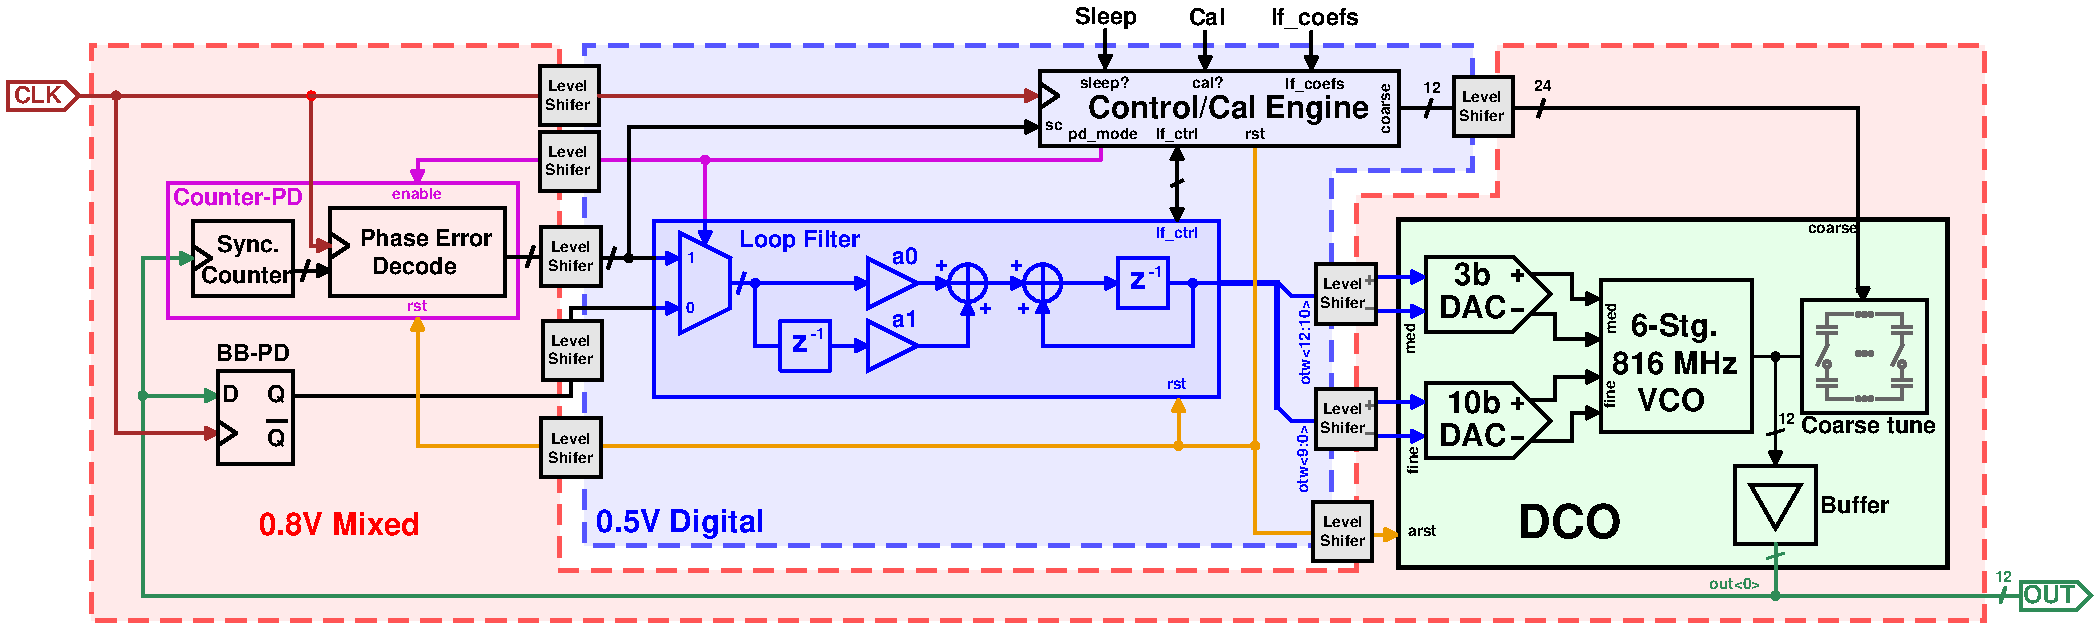
\includegraphics[width=1\textwidth, angle=0]{./figs/design/pll_master_arch_final}
			    \caption{ADPLL Architecture.}
			    \label{fig:pll_arch}
			\end{figure}
	The undertaken PLL architecture is in figure \ref{fig:pll_arch}. It comprises primarily of five components: (1) counter-based phase detector for initial start up, (2) bang-bang phase detector for steady state feedback, (3) proportional-integral controller loop filter, (4) DCO implemented as a VCO plus capacitive DACs, and (5) a control and calibration engine, consisting of digital logic. This design was achieved via minimization of complexity. First, the need of a divider is removed from the design by the usage of both the counter phase detector and BBPD. For initial cold start up of the PLL from an unknown state, the counter-based phase detector functions as a low-resolution replacement for a divider and linear phase detector. When near steady state, the counter-PD is disabled and replaced by BBPD feedback, which will maintain the PLL at steady state. The removal of a divider results in lower power consumption, and less noise added in-loop. The usage of only a BBPD in steady state further reduces power, as it is a minimum complexity phase detector. This is expected without significant performance degredation, as with proper optimization, BBPD PLLs can obtain comparable perform to linear charge-pump style PLLs \cite{xu_abidi_2017}. Additional power improvements are obtained in the usage of digital logic to implement the loop filter, using a simple PI-controller architecture. The final power saving move is implemented in a DCO based on the combination of several CDACs with a voltage controlled ring oscillator. This reduces to near zero the static curent draw associated with control of the VCO. The overall design is implemented with no static current paths, other than that associated with leakage, achieved by favoring static logic derived components throughout the PLL.


	A further feature gained in the proposed all-digital architecture is the ability to abruptly save the state of the PLL digitally and place it into an ultra low power sleep mode, and then later resume the PLL from the saved state. Figure \ref{fig:pll_sleep} demonstrate such operation, where $t_{l1}$ is the lock time from cold start, and $t_{l2}$ is the time to relock from a resume. This functionality enables the ability to rapidly duty cycle the PLL between active and sleep states, with minimal time to relock. Power consumption of the PLL is reduced by a factor that is the duty cycle which it is operated, and in this design can enable as low as 1$\mu$W power consumption as 1\% duty cycle. 

			\begin{figure}[htb!]
			        \centering
			        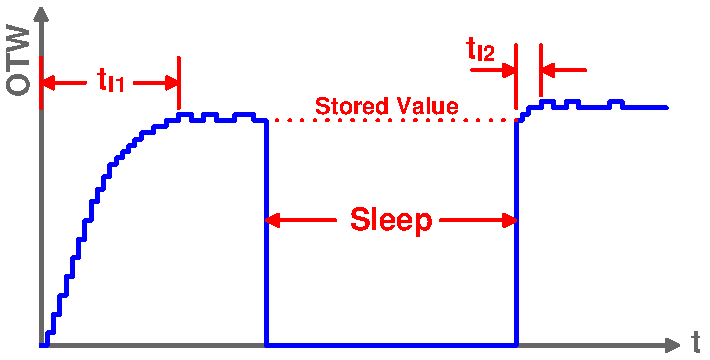
\includegraphics[width=0.6\textwidth, angle=0]{./figs/design/pll_sleep}
			    \caption{PLL sleep and resume operation.}
			    \label{fig:pll_sleep}
			\end{figure}


% \vspace{-2em}
% \begin{figure}[htb!]
% 	\center\fontfamily{\sfdefault}\selectfont
% XCircuit output "tdc_bbpll.tex" for LaTeX input from tdc_bbpll.ps
\def\putbox#1#2#3#4{\makebox[0.00000in][l]{\makebox[#1][l]{}\raisebox{\baselineskip}[0.00000in][0.00000in]{\raisebox{#2}[0.00000in][0.00000in]{\scalebox{#3}{#4}}}}}
\def\rightbox#1{\makebox[0.00000in][r]{#1}}
\def\centbox#1{\makebox[0.00000in]{#1}}
\def\topbox#1{\raisebox{-0.60\baselineskip}[0.00000in][0.00000in]{#1}}
\def\midbox#1{\raisebox{-0.20\baselineskip}[0.00000in][0.00000in]{#1}}
   \scalebox{1}{
   \normalsize
   \parbox{3.33750in}{
   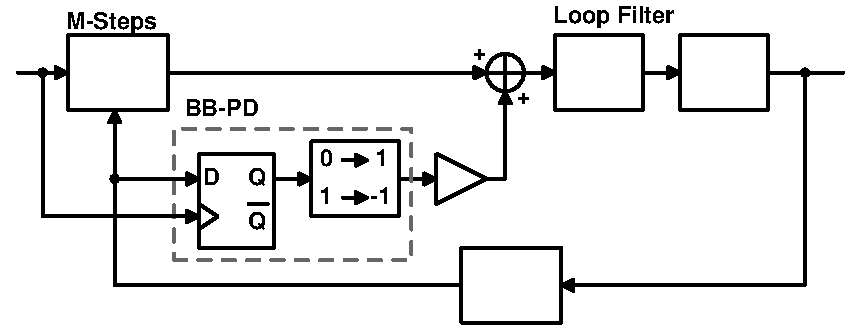
\includegraphics[scale=0.60000]{./figs/tdc_bbpll.pdf}\\
   % translate x=1412 y=528 scale 0.38
   \putbox{1.80600in}{0.70800in}{0.72}{$K_{bb}$}%
   \putbox{1.93200in}{0.14400in}{0.72}{$\div$ N}%
   \putbox{2.79600in}{0.99600in}{0.72}{DCO}%
   \putbox{2.24400in}{0.99600in}{0.72}{H$_{LF}$(z)}%
   \putbox{0.37200in}{0.99600in}{0.72}{TDC}%
   \putbox{0.03600in}{1.08600in}{0.72}{Clk}%
   \putbox{3.13200in}{1.08600in}{0.72}{Out}%
   } % close 'parbox'
   } % close 'scalebox'
   \vspace{-\baselineskip} % this is not necessary, but looks better
\fontfamily{\rmdefault}\selectfont

% 	\caption{PLL with parallel bang-bang phase detector and TDC.}
% 	\label{fig:tdc_bbpll}
% \end{figure}

The proposed digital architecture also enables a form of fast-locking via gear switching of the loop filter \cite{staszewski_balsara_2007}. In this work, the counter-based TDC is initially used for large frequency and phase errors with a loop filter optimized for speed, which after locking can be changed (gear-switched) to a BBPD optimized loop filter chosen to minimize total phase-noise. Design of optimal filters will be discused later on.

	
	\subsubsection{Power budget}
	The below power budget was used in the design process to divide up the 100 $\mu$W allotment between the different PLL components. In order to minimize oscillator phase noise, as large of a portion was allotted to the oscillator, being 80\%. 
		\begin{table}[htb!]
			\centering
			\def\arraystretch{1.5}		
			\setlength\arrayrulewidth{0.75pt}
			\setlength{\tabcolsep}{1em} % for the horizontal padding
			\begin{tabular}{|c|c|c|c|c|}
				\hline 
				\rule[-1ex]{0pt}{2.5ex} \cellcolor{gray!40}\textbf{DCO} & \cellcolor{gray!40}\textbf{Phase detector} & \cellcolor{gray!40}\textbf{Digital (LF)}& \cellcolor{gray!40}\textbf{Other} & \cellcolor{gray!40}\textbf{SUM} \\ 
				\hline 
				\rule[-1ex]{0pt}{2.5ex} 80 $\mu$W& 10 $\mu$W &  10 $\mu$W  & 0 $ \mu$W & $\leq$ 100  $\mu$W\\ 
				\hline 
			\end{tabular} 
			% \caption{Assigned specifications for branch line hybrid design.}
			% \label{asgn_specs}
		\end{table}   



	\subsubsection{Floorplan}
	The below floor plan (dimensions in microns) has been devised to meet the area requirement of $<$ 0.01 mm$^2$.
		\begin{figure}[htb!]
	        \centering
	        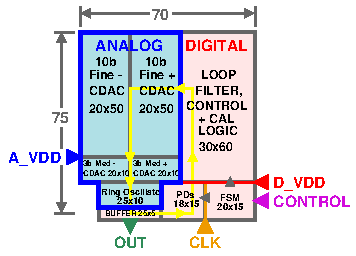
\includegraphics[width=0.6\textwidth, angle=0]{./figs/pll_floorplan2}
		    \caption{PLL floorplan.}
		\end{figure}

\subsubsection{Dividerless PLL}
\vspace{-2em}
\begin{figure}[htb!]
	\center\fontfamily{\sfdefault}\selectfont
% XCircuit output "bbpll_full_noise.tex" for LaTeX input from bbpll_full_noise.ps
\def\putbox#1#2#3#4{\makebox[0.00000in][l]{\makebox[#1][l]{}\raisebox{\baselineskip}[0.00000in][0.00000in]{\raisebox{#2}[0.00000in][0.00000in]{\scalebox{#3}{#4}}}}}
\def\rightbox#1{\makebox[0.00000in][r]{#1}}
\def\centbox#1{\makebox[0.00000in]{#1}}
\def\topbox#1{\raisebox{-0.60\baselineskip}[0.00000in][0.00000in]{#1}}
\def\midbox#1{\raisebox{-0.20\baselineskip}[0.00000in][0.00000in]{#1}}
   \scalebox{1}{
   \normalsize
   \parbox{5.50000in}{
   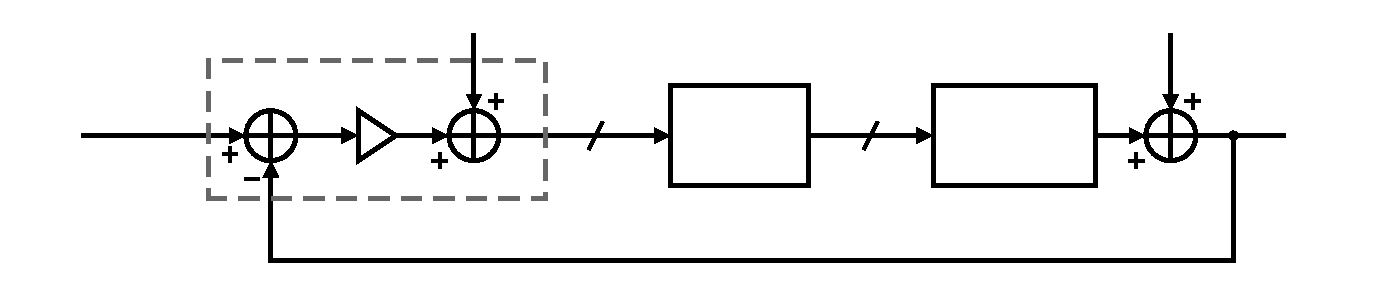
\includegraphics[scale=0.60000]{./figs/bbpll_full_noise.pdf}\\
   % translate x=416 y=448 scale 0.38
   \putbox{0.33600in}{0.70800in}{0.84}{$\Phi_{ref}$(t)}%
   \putbox{2.27400in}{0.73200in}{0.84}{e$_\Phi$(t)}%
   \putbox{1.42200in}{0.78600in}{0.84}{\rotatebox{-360}{$K_{BBPD}$}}%
   \putbox{1.20600in}{0.70800in}{0.84}{$\Phi_e$}%
   \putbox{0.83400in}{0.98400in}{0.84}{BBPD}%
   \putbox{2.77200in}{0.59400in}{0.84}{H$_{LF}$(s)}%
   \putbox{3.39600in}{0.72000in}{0.84}{u(t)}%
   \putbox{3.85800in}{0.60600in}{0.84}{$\frac{2\pi K_{DCO}}{s}$}%
   \putbox{4.82400in}{0.69600in}{0.84}{$\Phi_{out}$(t)}%
   \putbox{3.73200in}{0.87000in}{0.84}{DCO}%
   \putbox{1.93200in}{1.00800in}{0.84}{q$_{n_{BBPD}}$(t)}%
   \putbox{4.72200in}{1.00800in}{0.84}{$\Phi_{n_{DCO}}$(t)}%
   } % close 'parbox'
   } % close 'scalebox'
   \vspace{-\baselineskip} % this is not necessary, but looks better
\fontfamily{\rmdefault}\selectfont

	\caption{BBPD-PLL full noise model.}
	\label{fig:bbpll_full_noise}
\end{figure}

In the PLL theory (section \ref{sec:pll_output_noise}), the derived PLL detector phase noise component (equation \ref{eq:out_psd_bbpd_pll}) contains a term proportional to $N^2$, that is the detector noise will grow with the square of the PLL divider ratio. It is, however, possible to remove this $N^2$ dependency by usage of oscillator sub-sampling within the PLL \cite{Gao2015}. This is achieved by directly sampling the PLL output at a rate equivalent to the reference frequency. This is equivalent to removing the divider from the PLL loop and directly connecting the PLL output to the phase detector, which has been employed in this work (see figure \ref{fig:pll_arch}). To lock to the desired frequency, though, it must be guaranteed that the PLL frequency at the start of sub-sampling operation be within $f_{ref}/2$ of the target frequency (the PLL will lock to the nearest multiple of the reference frequency). In this work, this is achieved through sequencing at startup through two phase detectors. A synchronous counter phase detector (which emulates both a divider and phase detector) initially locks the PLL within $f_{ref}/2$ of the target frequency, after which the PLL is operated in sub-sampling bang-bang phase detector.

  In accordance to the change to a dividerless operation, the PLL closed loop transfer function has been rederived in equation \ref{eq:cont_pll_tf2}. Furthermore, new expressions for PLL output phase noise with a BBPD is given in equation \ref{eq:out_psd_bbpd_pll2}, and PLL output oscillator noise with a ring oscillator is given in equation \ref{eq:out_psd_dco_pll2}, for the noise model in figure \ref{fig:bbpll_full_noise}. Noise due to the loop filter here is ignored, as it will be possible to adjust the loop filter datapath resolution to make digital quantizaiton noise effects negligible.
		\begin{align} \label{eq:cont_pll_tf2}
			\mathrm{T}(s) = \frac{\Phi_{out}(s)}{\Phi_{ref}(s)} = \frac{2\pi K_{BBPD}K_{DCO}\sum_{j=0}^Z b_js^j}{\sum_{k=0}^P a_ks^{k+1} + 2\pi K_{BBPD}K_{DCO}\sum_{j=0}^Z b_js^j} = \frac{\mathrm{L}(s)}{1 + \mathrm{L}(s)}
		\end{align}
		\begin{align}\label{eq:out_psd_bbpd_pll2}
			S_{\Phi n_{BBPD,out}}(f) &= S_{n_{BBPD}}(f)\left|\frac{\Phi_{out}(f)}{q_{n_{BBPD}}(f)}\right|^2 = \frac{\left(\frac{\pi}{2}-1\right)}{f_{ref}}\left|\sigma_{\Phi_e}\mathrm{T}(f)\right|^2
		\end{align}
		\begin{align}\label{eq:out_psd_dco_pll2}
			S_{\Phi n_{DCO,out}}(f) &= \mathcal{L}_{min}(f)\left|\frac{\Phi_{out}(f)}{q_{n_{DCO}}(f)}\right|^2 = \frac{7.33k_BT}{P}\left(\frac{f_0}{f}\right)^2|1-\textnormal{T}(f)|^2 
		\end{align}

% ################################################################################################
% ################################################################################################
	\subsection{Bang-Bang Phase Detector}
		A bang-bang phase detector, as introduced in section \ref{bbpd_theory}, can be implemented physically with a D flip-flop \cite{Razavi2020} and logic to map the logical state to a signed $\pm$1 value that may be passed into a digital loop filter. This is shown in figure \ref{fig:bbpd_dff}. 

		\begin{figure}[htb!]
			\center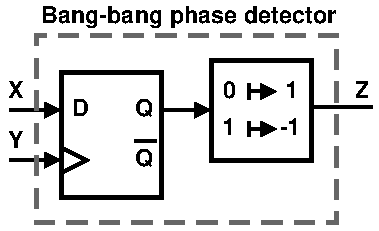
\includegraphics[width=0.4\textwidth, angle=0]{./figs/design/bbpd_}
			\caption{Bang-bang phase detector with D flip-flop.}
			\label{fig:bbpd_dff}
		\end{figure}
		The realization of a BBPD using a digital flip flop introduces additional noise to the system in the form of jitter. Jitter arises as an artifact of circuit and supply noise. For small time differentials between the BBPD inputs X and Y, the output can be stochatically corrupted due to the presence of noise. Furthermore, physical D flip flop implementations exhibit set-up and hold time requirements for data to be stable (to allow internal nodes to settle), so deterministic corruption of phase detection can be imparted if the inputs violate physical timing requirements. These sources of corruption cause BB-PD transfer characteristics in terms of output expectation, $\mathbb{E}[Z]$, with respect to input timing difference $\Delta t_{XY}$ to deviate from an ideal step response, demonstrated in figure \ref{fig:bbpd_jit_pdf}. Analytically, the corruption of the transfer characteristic can be viewed as being caused by an additive phase noise component before the signum operation in the BBPD, as shown in figure \ref{fig:bbpd_noise_nonlinear}. The expectation $\mathbb{E}[Z(\Delta t_{XY})]$ acts as a cumulative distribution function (CDF) for this phase noise component. Thus, differentiation of $\mathbb{E}[Z(\Delta t_{XY})]$ results in a probability distribution function (PDF) P(T=$\Delta t_{xy}$) of this phase noise signal. Statistical analysis of variance of the PDF provides an RMS value for timing jitter of this additive noise source, $\sqrt{\mathrm{Var}[T]} = \sigma_{t,j}$. The RMS timing jitter may be converted to RMS phase error of the noise source as $\sigma_{\Phi_j} = 2\pi f_{osc}\sigma_{t_j}$. This analysis approach is applied in this work to evaluate BBPD performance.
 
		\begin{figure}[htb!]
		    \centering
			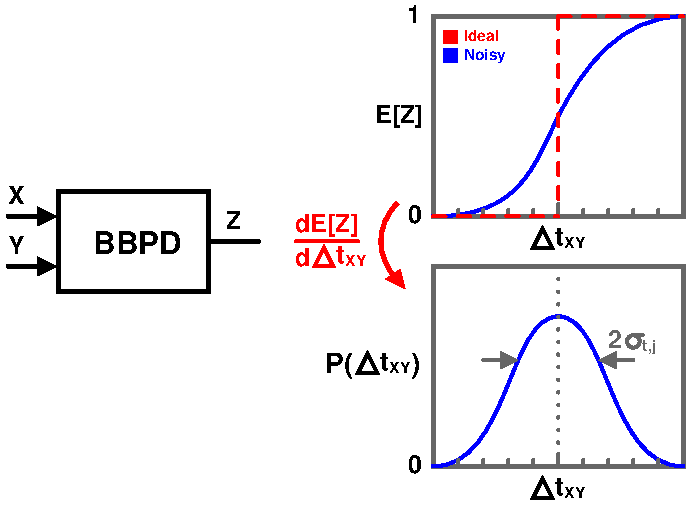
\includegraphics[width=0.6\textwidth, angle=0]{./figs/bbpd_jitter.pdf}
			\caption{BBPD output expectation and jitter PDF versus input time differential.}
			\label{fig:bbpd_jit_pdf}
		\end{figure}

	\begin{figure}[htb!]
	    \centering
	    \begin{subfigure}{0.5\textwidth}
	        \centering
	        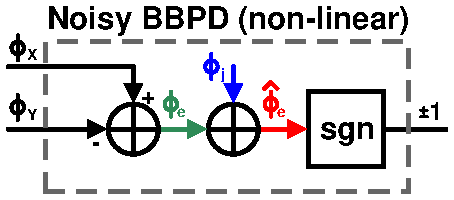
\includegraphics[width=0.8\textwidth, angle=0]{figs/design/bbpd_noise_nonlinear}
	        \caption{ }
	        \label{fig:bbpd_noise_nonlinear}
	    \end{subfigure}%
	    \begin{subfigure}{0.5\textwidth}
	        \centering
	        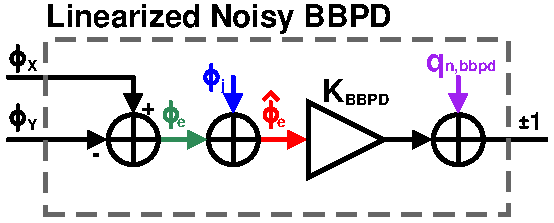
\includegraphics[width=0.9\textwidth, angle=0]{figs/design/bbpd_noise_linear}
	        \caption{ }
	        \label{fig:bbpd_noise_linear}
	    \end{subfigure}
	    % \caption{x.}
	    \caption{\textbf{(a)} Noisy BBPD nonlinear model \textbf{(b)} Noisy BBPD linearized model}
	     \label{fig:bbpd_noisy}
	\end{figure} 

	With a model for BBPD noise due to implementation non-idealities, a modified linearized model for the BBPD will be established here. This model will reconcile the ideal BBPD noise introduced in section \ref{sec:bbpd_noise} with the noise due to the new additive jitter component just described. First, a component representing the non-ideal jitter component, $\Phi_j$, is added into noise model from figure \ref{fig:bbpll_full_noise}. The result is the linearized model of figure \ref{fig:bbpd_noise_linear}. We then define a modified phase error, $\hat{\Phi}_e$, which includes the nominal $\Phi_e$ and the jitter corruption:
	\begin{equation}
	\hat{\Phi}_e = \Phi_e + \Phi_j.
	\end{equation}
	$\hat{\Phi}_e$ has a variance defined as $\sigma_{\hat{\Phi}_e}^2 = \sigma_{\Phi_e}^2 + \sigma_{\Phi_j}^2$, assuming $\Phi_e$ and $\Phi_j$ are uncorrelated. Defining BBPD gain in terms of $\sigma_{\hat{\Phi}_e}$:
	\begin{equation}
		K_{BBPD} = \sqrt{\frac{2}{\pi}}\cdot\frac{1}{\sigma_{\hat{\Phi}_e}} = \sqrt{\frac{2}{\pi}}\cdot\frac{1}{\sqrt{\sigma_{\Phi_e}^2 + \sigma_{\Phi_j}^2}}
	\end{equation}

	 It is then observed that the output Z is valued $\pm$1, thus its power is always $\sigma_Z^2$=1. Furthermore:
	\begin{equation}
	 	\sigma^2_{Z} = 1 = K_{BBPD}^2(\sigma^2_{\phi_e} +\sigma^2_{\phi_j})  + \sigma^2_{q_{n,BBPD}}
	\end{equation}
	 As determined in section \ref{sec:bbpd_noise}, it is inherent that $\sigma^2_{q_{n,BBPD}} = 1 - \frac{2}{\pi}$. If the total output noise
			\begin{equation}
				\sigma^2_{\phi_{n,BBPD}} =  \sigma^2_{q_{n,BBPD}} + K_{BBPD}^2\sigma^2_{\phi_j} =  1 - \frac{2}{\pi}\frac{\sigma^2_{\phi_e}}{\sigma^2_{\phi_j} + \sigma^2_{\phi_e}}
			\end{equation}
	If the BB-PD is connected directly to oscillator output, $\sigma^2_{\phi_e}$ = $\sigma^2_{\phi_n}$, i.e. the PLL output phase noise. The spectral density of the BB-PD phase noise is then:
		\begin{equation}
			S_{\phi_{n,BBPD}} = \frac{\sigma^2_{\phi_{n,BBPD}}}{f_{ref}} =  \frac{1 - \frac{2}{\pi}\frac{\sigma^2_{\phi_n}}{\sigma^2_{\phi_j} + \sigma^2_{\phi_n}}}{f_{ref}}
		\end{equation}

		\begin{align}\label{eq:out_psd_bbpd_pll3}
			S_{\Phi n_{BBPD,out}}(f) &= S_{n_{BBPD}}(f)\left|\frac{\Phi_{out}(f)}{q_{n_{BBPD}}(f)}\right|^2 = \frac{\frac{\pi}{2}(\sigma^2_{\phi_j} + \sigma^2_{\phi_n})-\sigma^2_{\phi_n}}{f_{ref}}\left|\mathrm{T}(f)\right|^2
		\end{align}

	% \begin{itemize}[itemsep=4pt,label=\protect---]
	% 	\item It is observed that PLL phase noise spectrum is approximately Lorentzian (except for peaking and flicker noise components). Given BB-PD noise PSD of $S_{\phi_{n,BBPD}}$, and an oscillator with noise PSD $S_{\phi_{n,osc}}(\Delta f)$, the optimal bandwidth for minimum noise power is:

	% 	\begin{equation}
	% 		BW_{opt} =  \sqrt{\frac{S_{\phi_{n,osc}}(\Delta f)}{S_{\phi_{n,BBPD}}}}\Delta f
	% 	\end{equation}
	% 	\item The total PLL output phase noise with optimal bandwidth is then:

	% 	\begin{equation}
	% 		\sigma^2_{\phi_{n,opt}} =   \pi\sqrt{\phi_{n,osc}(\Delta f)S_{\phi_{n,BBPD}}}\Delta f
	% 	\end{equation}
	% \end{itemize}
	% \vspace{-3em}
	% \begin{figure}[htb!]
	%     \centering
	%     \begin{subfigure}{0.33\textwidth}
	%         \centering
	%         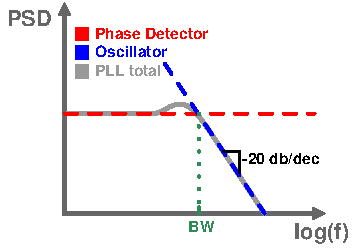
\includegraphics[width=1\textwidth, angle=0]{./figs/pll_spectrum_lorentzian.pdf}
	%     \end{subfigure}%
	%     \begin{subfigure}{0.33\textwidth}
	%         \centering
	%         \center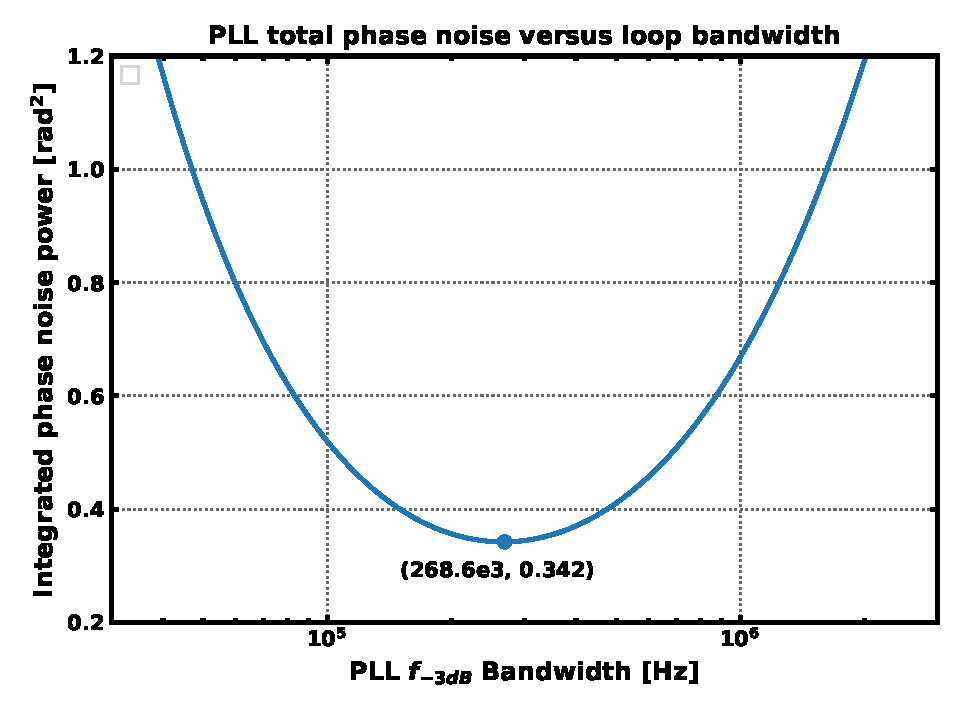
\includegraphics[width=1.0\textwidth, angle=0]{./figs/bandwidth_vs_pn.pdf}
	%     \end{subfigure}
	%     % \caption{Approximate model for ring oscillator inverter delay cell.}
	% \end{figure}




	% \begin{itemize}[itemsep=4pt,label=\protect---]
	% 	\item Using the findings for BB-PD noise PSD, assumption of Lorentzian spectrum, and constraint that BW = $\alpha f_{ref}$ (recommended $\alpha$$<$0.1 [2], rule of thumb since ancient PLL days). Given oscillator center frequency $f_c$, BB-PD jitter is constrained:

	% 	\begin{equation}
	% 		\sigma_{t_j} \leq \frac{\sigma_{\Phi_n}}{2\pi f_c}\sqrt{\frac{2}{\pi}\left(\frac{1}{\pi\alpha} - \frac{\pi}{2} + 1\right)} = \frac{\sigma_{\Phi_n}}{2\pi f_c}\beta(\alpha)
	% 	\end{equation}
	% 	\item $\beta(\alpha=0.1)$ = 1.28, $\beta(\alpha=0.05)$ = 1.92.
	% 	\item Using my PLL specifications ($f_c$ = 2.448 GHz, CNR = -$\sigma_{\Phi_n}$ = 17 dB, $\alpha=0.1$), {\color{red}\textbf{$\sigma_{t,j}\leq 11.8 $ ps}}
	% \end{itemize}



	% \begin{itemize}[itemsep=4pt,label=\protect---]
	% 	\item With an unconstrained relationship for BW and $f_{ref}$, and the optimal bandwidth finding, it is determined that the optimal value of $\sigma_{t,j}$ for minimum phase noise is:

	% 	\begin{equation}
	% 		\sigma_{t_j,opt} = \frac{\sigma_{\Phi_n}}{2\pi f_c}\sqrt{\frac{2}{\pi}\left[\frac{\sigma^4_{\Phi_n} f_{ref}}{\pi^2 S_{\phi_{n,osc}}(\Delta f) \Delta f^2} - \left(\frac{\pi}{2} - 1\right)\sigma^2_{\Phi_n}\right]}
	% 	\end{equation}

	% \end{itemize}

	% \begin{itemize}[itemsep=4pt,label=\protect---]
	% 	\item Setting the two jitter equations of the last side equal, it is found that optimal phase noise power is:

	% 	\begin{equation}
	% 		\sigma^2_{\Phi_n, opt} = \frac{\pi S_{\phi_{n,osc}}(\Delta f) \Delta f^2}{\alpha f_{ref}}
	% 	\end{equation}
	% 	\item The optimal reference frequency ($\sigma_{\Phi_n}=2\pi f_c \sigma_{t_n}$ = CNR):
	% 	\begin{equation}
	% 		f_{ref} = \frac{\pi S_{\phi_{n,osc}}(\Delta f) \Delta f^2}{\alpha \sigma^2_{\Phi_n}}
	% 	\end{equation}
	% 	\item The optimal oscillator phase noise at offset $\Delta f$:
	% 	\begin{equation}
	% 		S_{\phi_{n,osc}}(\Delta f) = \frac{\alpha f_{ref}\sigma^2_{\Phi_n}}{\pi \Delta f^2} 
	% 	\end{equation}
	% 	\item For CNR = 17 dB, $S_{\phi_{n,osc}}(\Delta f = 1 MHz)$ = -80 dBc/Hz, $\alpha$ = 0.1, {\color{red}the optimal $f_{ref}$ = 15.7 MHz.}
	% 	\item For CNR = 20 dB, $S_{\phi_{n,osc}}(\Delta f = 1 MHz)$ = -80 dBc/Hz, $\alpha$ = 0.1, {\color{red}the optimal $f_{ref}$ = 31.4 MHz.}
	% \end{itemize}


		\FloatBarrier






		\subsubsection{Circuit}
		The physcial implementation of the bang-bang phase detector has been selected to utilize a true single phase clock (TSPC) D-flip flop \cite{Yuan1989}. The positive-edge triggered variant of this circuit has been implemented as shown in figure \ref{fig:tspc_dff}. Selection of this topology was based on the desire for the usage of a single ended clock as a reference signal.

			\begin{figure}[htb!]
			        \centering
			        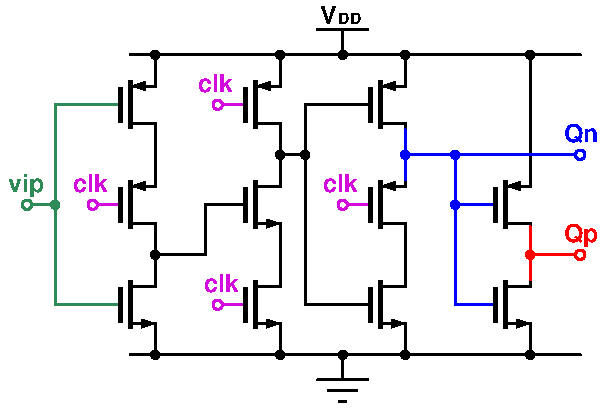
\includegraphics[width=0.6\textwidth, angle=0]{./figs/design/tspc_}
			    \caption{True single-phase clock (TSPC) D flip-flop, positive edge triggered.}
			    \label{fig:tspc_dff}
			\end{figure}

		This TSPC design was validated in simulation with RVT devices with all devices set with (W/L) = \{100n/20n, 200n/20n\}, and with supply voltages of 0.5 and 0.8 volts. Results for jitter PDF are in figure \ref{fig:tspc_dff_sim}, and the RMS jitter and power consumption are in table \ref{tab:dff}. For implementation (W/L) = 100n/20n was selected for all devices, as to ensure that the budgeted power of 10 $\mu$W is met with layout parasitics. 


		% \end{itemize}
		% % \vspace{-3em}
		% \begin{figure}[htb!]
		%     \centering
		%     \begin{subfigure}{0.5\textwidth}
		%         \centering
		%         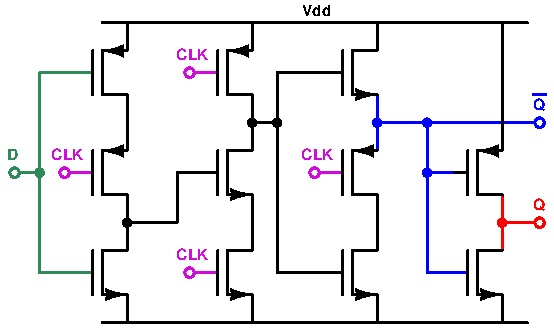
\includegraphics[width=0.8\textwidth, angle=0]{./figs/tspc_dff.pdf}
		%         \caption{TSPC DFF}
		%     \end{subfigure}%
		%     \begin{subfigure}{0.5\textwidth}
		%         \centering
		%         \center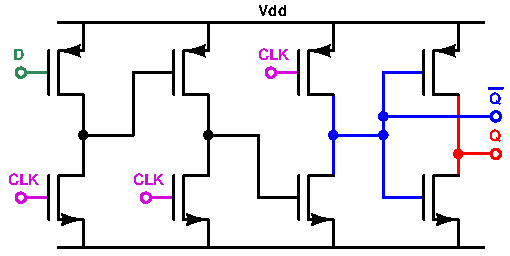
\includegraphics[width=0.8\textwidth, angle=0]{./figs/etspc_dff.pdf}
		%         \caption{e-TSPC DFF}
		%     \end{subfigure}
		%     % \caption{Approximate model for ring oscillator inverter delay cell.}
		% \end{figure}


	% \begin{itemize}[itemsep=4pt,label=\protect---]
	% 	\item Utilized TSPC DFF, with inverter buffers (FETs sized 200n/20n) for clock and data buffers.
	% 	\item Sweep delay between inputs, calculating the expect value of the output for 100 bits. Transient noise simulated (up to 100 GHz), and the inital state of the FF is set to be high 50x and low 50x to include hysteresis effects. 
	% 	\item V$_{DD} \in$ \{0.5, 0.8\} V and (W/L) $\in$ \{100n/20n, 200n/20n\} tested. 100 aF added to every node.
	% 	\item \textbf{Resulting CDFs of the input time delta versus output expectation are below.}
	% \end{itemize}
	% \vspace{-2em}
	% \begin{figure}[htb!]
	%     \centering
	% 	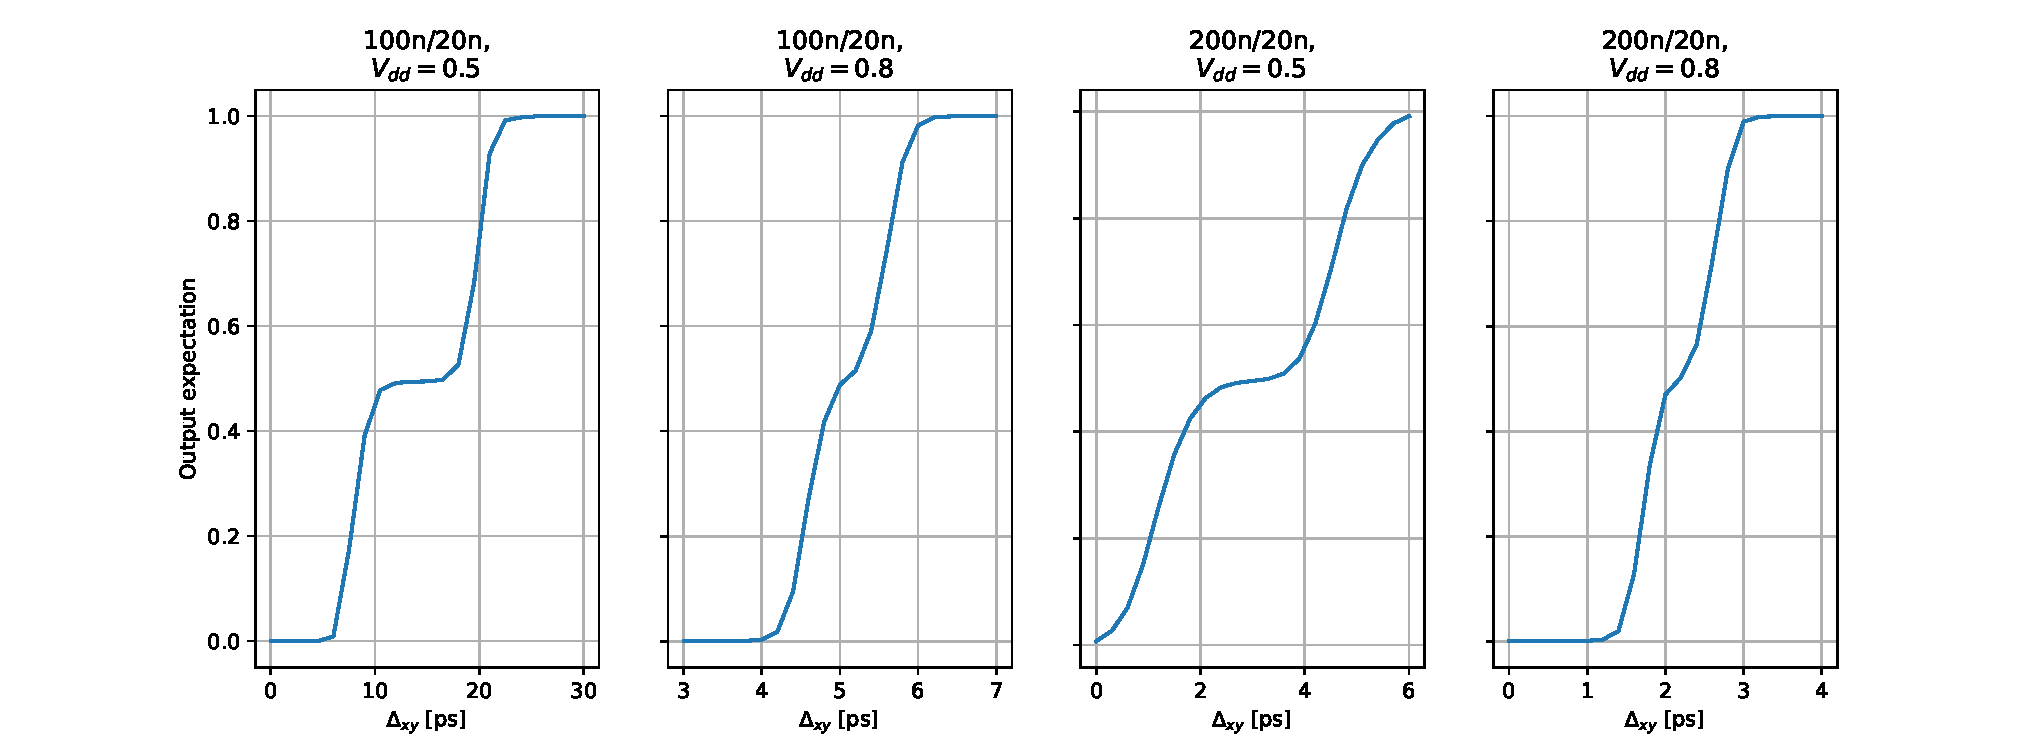
\includegraphics[width=1\textwidth, angle=0]{./figs/cdfs.pdf}
	% \end{figure}

	% \begin{itemize}[itemsep=4pt,label=\protect---]
	% 	\item Jitter PDFs are bimodal from hysteresis of DFF. 
	% 	\item Increasing (W/L) or $V_{DD}$ both impact jitter favorably.
	% 	\item \textbf{The jitter PDF (computed from the CDFs) of the input time delta versus output expectation are below. (Delays are removed)}
	% \end{itemize}
	% \vspace{-2em}
	\begin{figure}[htb!]
	    \centering
		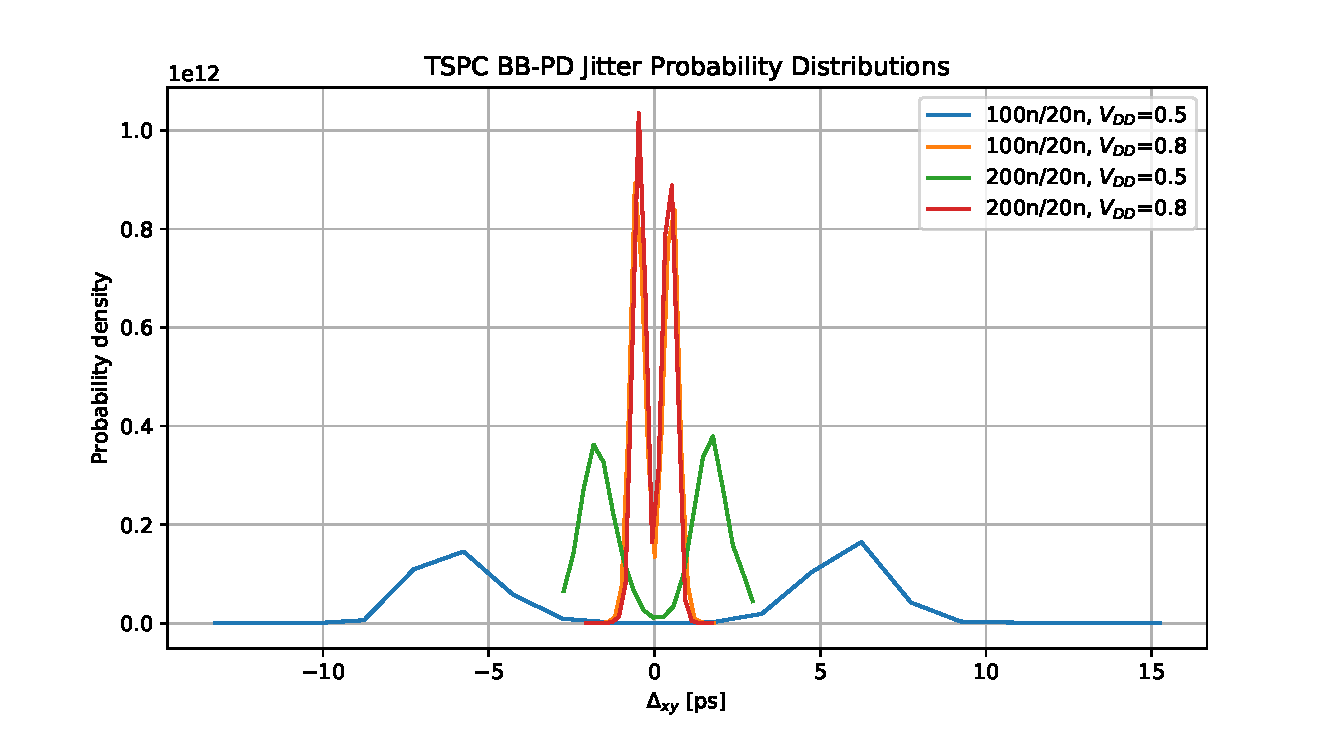
\includegraphics[width=0.7\textwidth, angle=0]{./figs/jitter_pdfs.pdf}
		\caption{Jitter PDF from simulated TSPC DFFs.}
		\label{fig:tspc_dff_sim}
	\end{figure}


		\begin{table}[h!]
			\centering
			\def\arraystretch{1.5}		
			\setlength\arrayrulewidth{0.75pt}
			\setlength{\tabcolsep}{1em} % for the horizontal padding
			\begin{tabular}{|c|c|c|c|}
				\hline 
				\rule[-1ex]{0pt}{2.5ex} \cellcolor{gray!40}\textbf{(W/L)} & \cellcolor{gray!40}\textbf{Supply [V]} & \cellcolor{gray!40}\textbf{RMS jitter [ps]}& \cellcolor{gray!40}\textbf{Power [$\mu$W]}\\ 
				\hline 
				\rule[-1ex]{0pt}{2.5ex} 100n/20n  & 0.5 & 6.01 & 1.64\\ 
				\hline 
				\rule[-1ex]{0pt}{2.5ex} 100n/20n  & 0.8 & 0.832  & 3.942\\ 
				\hline 
				\rule[-1ex]{0pt}{2.5ex} 200n/20n  & 0.5 & 1.776 & 2.215 \\ 
				\hline 
				\rule[-1ex]{0pt}{2.5ex} 200n/20n  & 0.8 & 0.496  & 4.591 \\ 
				\hline 
			\end{tabular} 
			\caption{Schematic simulation of TSPC DFF.}
			\label{tab:dff}
		\end{table}   







		\FloatBarrier
		\subsubsection{Layout}
			\hl{Area?}
			\begin{figure}[htb!]
			        \centering
			        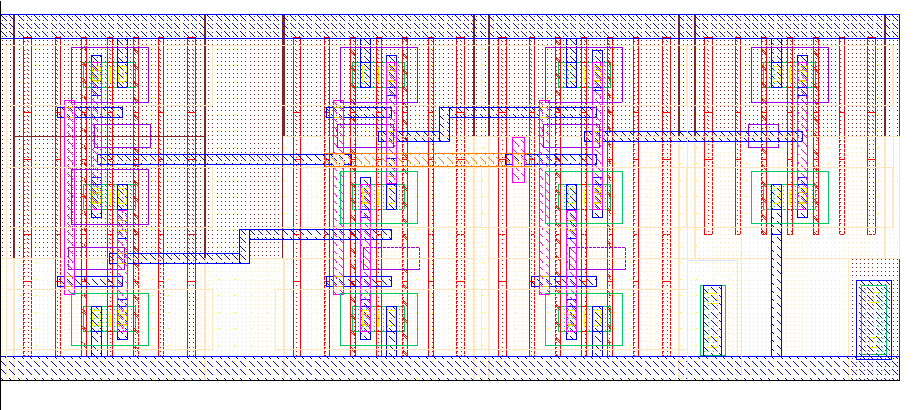
\includegraphics[width=\textwidth, angle=0]{./figs/layout/layout_bbpd}
			    \caption{Single ended bang-bang phase detector.}
			\end{figure}

% ################################################################################################
% ################################################################################################


% ################################################################################################
% ################################################################################################
	\FloatBarrier
	\subsection{Loop Filter}
	For selection of a loop filter, some basic criteria have been selected:
	\begin{enumerate}[itemsep=0pt,label=\protect\mycirc{\arabic*}]
		\setlength\itemsep{-0.8em}
		\item Zero steady state phase error, to ensure accuracy of synthesized frequency.
		\item Minimize complexity of implemented logic, i.e. minimize the number of poles and zeros.
		\item Low pass response of PLL in closed-loop.
	\end{enumerate}
	From this author's previous work \cite{Me}, it was established that the pole-zero filter satisfying these requirements is a proportional-integral controller.

\subsubsection{Proportional-integral Loop Filter}
 A proportional-integral controller \cite{ogata_2010_pid} is given in equation \ref{eq:pi_pll_tf}, containing an proportional gain term $K_p$, and an integral gain term $K_p$. This can be optionally represented using a pole at zero and a zero with $\omega_z = K_i/K_p$:
			\begin{equation} \label{eq:pi_pll_tf}
				\textnormal{H}_{LF}(s) = K_p + \frac{K_i}{s}  = \frac{K_i}{s}\left(\frac{s}{\omega_z} + 1\right) 
			\end{equation}
			Substitution of this controller into the PLL closed loop transfer function (equation \ref{eq:cont_pll_tf2}) results in:
			\begin{equation}\label{eq:pi_bbpdpll_tf}
				T(s) = \frac{\Phi_{out}(s)}{\Phi_{ref}(s)} =  \frac{ 2\pi K_{BBPD}K_{DCO}K_{i} \left(\frac{s}{\omega_z} + 1\right) }{s^2 + 2\pi K_{BBPD}K_{DCO}K_{i}\left(\frac{s}{\omega_z} + 1\right) }
			\end{equation}
\subsubsection{Optimal Filter Selection}
			Optimization of loop filter will be attempted to minimizing the total integrated phase noise power out of the PLL, while keeping the filter bandwidth low enough to acheive satisfactory oversampling for acceptable performance. A limit of loop bandwidth $BW_{loop}$ = 0.1$f_{ref}$ is employed here, which is a figure commonly cited in PLL literature from \cite{gardner_1980}. Higher degrees of oversampling lead to deviations between continuous PLL models and real sampled-PLL performance. 

			First, some mathematical simplifications of the PLL model are introduced. Rewriting equation \ref{eq:pi_bbpdpll_tf} with substitutions $\omega_z = K_i/K_p$ and $\mathrm{K} = 2\pi K_{BBPD}K_{DCO}K_{i}$:
			\begin{equation} \label{eq:simp_pi_pll_tf}
				T(s) = \frac{\Phi_{out}(s)}{\Phi_{ref}(s)} = \frac{s\frac{K}{\omega_z} + K }{s^2 + s\frac{K}{\omega_z} + K}
			\end{equation}
			The denominator can be redefined in terms of a natural frequency $\omega_n$ and damping ratio $\zeta$:
			\begin{equation}
				s^2 + s\frac{K}{\omega_z} + K = s^2 + s2\zeta\omega_n + \omega_n^2
			\end{equation}
			Thus, $\omega_n = \sqrt{K}$, and $\omega_z = \sqrt{K}/2\zeta$. The poles of equation \ref{eq:simp_pi_pll_tf} are then located at s = $\zeta\sqrt{K} \pm j\sqrt{K}\sqrt{1-\zeta^2}$. The settling time constant of the PLL is determined by the real portion of dominant pole of equation \ref{eq:simp_pi_pll_tf}:
			\begin{equation}
				\tau = \frac{1}{|\min(\Re(\{s_{p1}, s_{p2}\}))|}
			\end{equation}
			 It is decidedly of interest to minimize settling time of the PLL (i.e. time constant), thus maximizing the frequency of the dominant pole of the PLL is of interest. Based on the pole-zero plot of figure \ref{fig:pi_pll_pz}, it is seen the dominant pole of equation \ref{eq:simp_pi_pll_tf} is maximized with $\zeta=1$. The shown pole and zero loci are oriented based on increasing $\zeta$ values. According to Razavi \cite{razavi_2017}, $\zeta$ is usually 
			"chosen to be $>\sqrt{2}/2$ or even 1 to avoid excessive ringing." It has according been chosen to fix $\zeta=1$ for the PI-controller. 
			\begin{figure}[htb!]
				\center\fontfamily{\sfdefault}\selectfont
% XCircuit output "pi_pz_plot.tex" for LaTeX input from pi_pz_plot.ps
\def\putbox#1#2#3#4{\makebox[0.00000in][l]{\makebox[#1][l]{}\raisebox{\baselineskip}[0.00000in][0.00000in]{\raisebox{#2}[0.00000in][0.00000in]{\scalebox{#3}{#4}}}}}
\def\rightbox#1{\makebox[0.00000in][r]{#1}}
\def\centbox#1{\makebox[0.00000in]{#1}}
\def\topbox#1{\raisebox{-0.60\baselineskip}[0.00000in][0.00000in]{#1}}
\def\midbox#1{\raisebox{-0.20\baselineskip}[0.00000in][0.00000in]{#1}}
   \scalebox{1}{
   \normalsize
   \parbox{4.20000in}{
   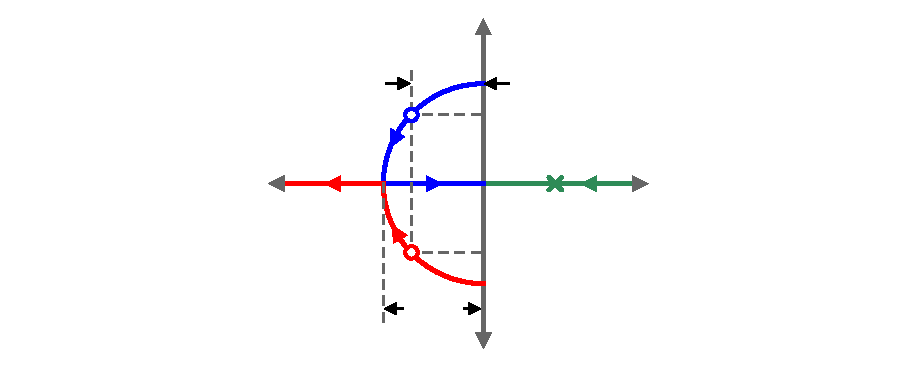
\includegraphics[scale=0.70000]{./figs/pi_pz_plot.pdf}\\
   % translate x=800 y=416 scale 0.38
   \putbox{2.85600in}{0.67900in}{1.20}{$\Re(s)$}%
   \putbox{2.30300in}{1.52600in}{1.20}{$\Im(s)$}%
   \putbox{1.89000in}{0.21700in}{1.20}{$\sqrt{\mathrm{K}}$}%
   \putbox{1.45600in}{1.36500in}{1.20}{$\zeta\sqrt{\mathrm{K}}$}%
   \putbox{2.38700in}{0.95900in}{1.20}{$\sqrt{\mathrm{K}}/2\zeta$}%
   } % close 'parbox'
   } % close 'scalebox'
   \vspace{-\baselineskip} % this is not necessary, but looks better
\fontfamily{\rmdefault}\selectfont

				\caption{PI-controller PLL pole-zero locations.}
				\label{fig:pi_pll_pz}
			\end{figure}
			\FloatBarrier
			To illustrate the effect of the damping ratio $\zeta$, figure \ref{fig:pi_pll_response} illustratesexample frequency and step responses of a PI-controlled PLL. It is observed that increasing ringing and peaking is obtained with increasing values of $\zeta$. This is undesirable from a stability standpoint, and increased peaking in the PLL transfer function will increase output phase noise contributions, also undesirable. Therefore, the selection of $\zeta=1$ is solidified.
			\begin{figure}[htb!]
				\center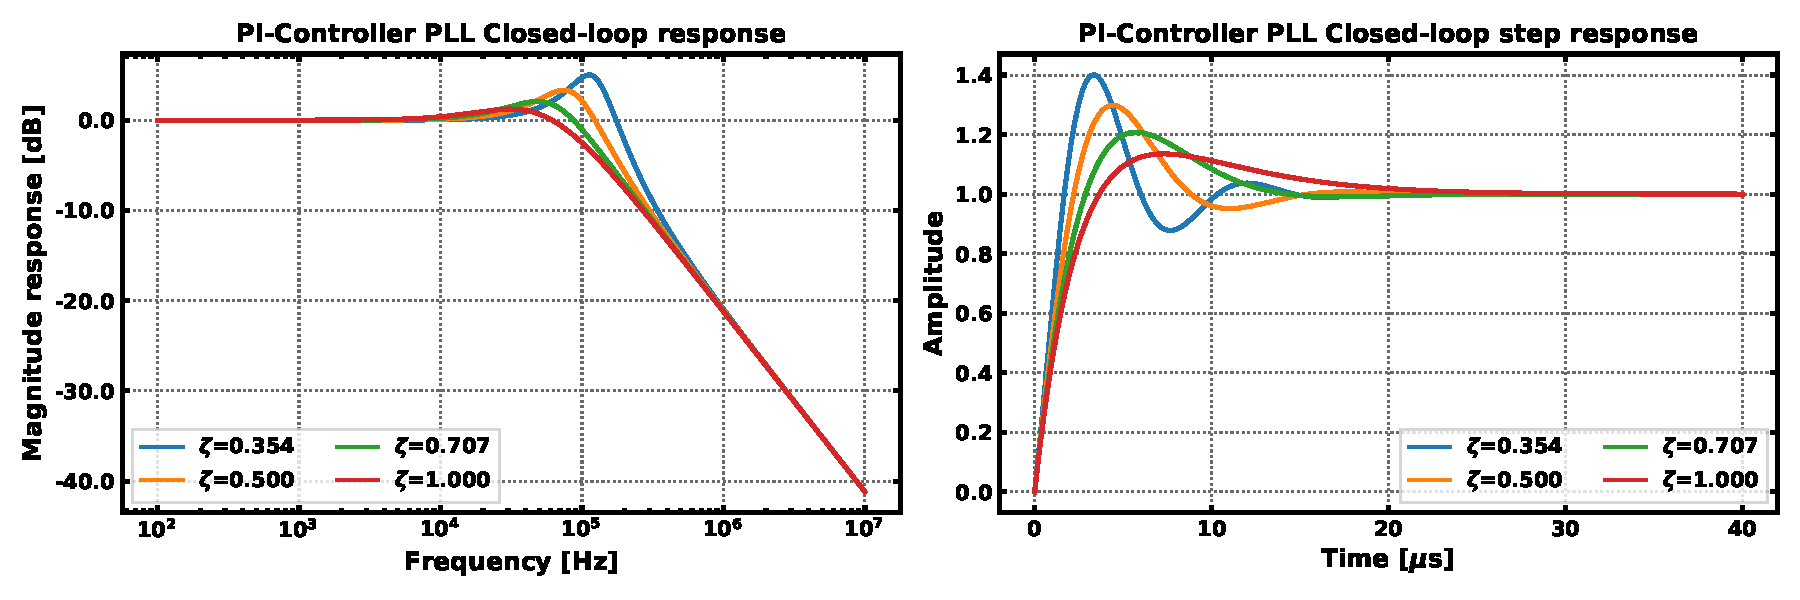
\includegraphics[width=1.0\textwidth, angle=0]{figs/pi_pll_response.pdf}
				\caption{Example PI-PLL responses with varied $\zeta$.}
				\label{fig:pi_pll_response}
			\end{figure}
			\FloatBarrier
			With $\zeta$ is constrained to 1, the final simplified PLL closed loop transfer function is in equation \ref{eq:simp_pi_pll_tf_z1}. The form of this equation is favorable for integration, due to the selection of $\zeta$=1.
			\begin{equation} \label{eq:simp_pi_pll_tf_z1}
				T(s) = \frac{2\sqrt{K}s + K }{s^2 + 2\sqrt{K}s + K}
			\end{equation}
			
			Now, the PLL output referred noise power of the oscillator and BBPD may be calculated. First, if the PLL-less oscillator is defined as equation \ref{eq:osc_spectrum}, where $S_{0_{osc}}$ is defined as the oscillator spectral density at 1 Hz frequency offset from the carrier. 
			\begin{equation}\label{eq:osc_spectrum} 
				\mathcal{L}(f) = \frac{S_{0_{osc}}}{f^2} 
			\end{equation} 
			The PLL output spectum is then computed as: 
			\begin{align}\label{eq:out_psd_dco_pll3} 
				S_{\Phi n_{DCO,out}}(f) &= \frac{S_{0_{osc}}}{f^2}|1-\textnormal{T}(f)|^2  
			\end{align} Now, $|1-\textnormal{T}(f)|^2$ is found to be after much simplification:
			\begin{equation} |1-\textnormal{T}(f)|^2 =
				\frac{f^4}{\left(f^2+\frac{K}{(2\pi)^2}\right)^2} 
			\end{equation} 

			Thus, re-evaluating equation \ref{eq:out_psd_dco_pll3} yields:
			\begin{align}\label{eq:out_psd_dco_pll4} 
				S_{\Phi n_{DCO,out}}(f) &= S_{0_{osc}}\frac{f^2}{\left(f^2+\frac{K}{(2\pi)^2}\right)^2} 
			\end{align} 

			The total PLL phase noise power associated with the oscillator, $\sigma_{\Phi_{n,DCO}}^2$ is achieved by integrating equation \ref{eq:out_psd_dco_pll4} with respect to frequency.
			\begin{align}\label{eq:out_psd_dco_pll4} \sigma_{\Phi_{n,DCO}}^2 =
				\int_{-\infty}^{\infty} S_{\Phi n_{DCO,out}}(f)df &=
				S_{0_{osc}}\int_{-\infty}^{\infty}\frac{f^2}{\left(f^2+\frac{K}{(2\pi)^2}\right)^2}df
				\\ &= S_{0_{osc}}\frac{\pi^2}{\sqrt{K}} 
			\end{align} 

			Next, the total BBPD noise at the PLL output is computed. The expression for BBPD noise density in equation \ref{eq:out_psd_bbpd_pll3} will be used, and for which $|\textnormal{T}(f)|^2$ must be computed. This is: 
			\begin{equation} 
				|\textnormal{T}(f)|^2 =
				\frac{4\frac{K}{(2\pi)^2}f^2 +
				\frac{K^2}{(2\pi)^4}}{\left(f^2+\frac{K}{(2\pi)^2}\right)^2} 
			\end{equation}

			The resulting BBPD spectral density equation is:
			\begin{align}\label{eq:out_psd_bbpd_pll4} 
				S_{\Phi n_{BBPD,out}}(f) & =
				\frac{\frac{\pi}{2}(\sigma^2_{\phi_j} +
				\sigma^2_{\phi_n})-\sigma^2_{\phi_n}}{f_{ref}}\left|\mathrm{T}(f)\right|^2
				\\&= \frac{\frac{\pi}{2}(\sigma^2_{\phi_j} +
				\sigma^2_{\phi_n})-\sigma^2_{\phi_n}}{f_{ref}}\cdot\frac{4\frac{K}{(2\pi)^2}f^2
				+ \frac{K^2}{(2\pi)^4}}{\left(f^2+\frac{K}{(2\pi)^2}\right)^2} 
			\end{align} 

			The total PLL phase noise power associated with the BBPD, $\sigma_{\Phi_{n,BBPD}}^2$ is achieved by integrating equation \ref{eq:out_psd_bbpd_pll4} with respect to frequency:
			\begin{align}\label{eq:out_psd_bbpd_pll4} 
				\sigma_{\Phi_{n,BBPD}}^2 & =
				\frac{\frac{\pi}{2}(\sigma^2_{\phi_j} +
				\sigma^2_{\phi_n})-\sigma^2_{\phi_n}}{f_{ref}}\int_{-\infty}^{\infty}\frac{4\frac{K}{(2\pi)^2}f^2
				+ \frac{K^2}{(2\pi)^4}}{\left(f^2+\frac{K}{(2\pi)^2}\right)^2}df\\ &= 
				\frac{5\sqrt{K}}{4f_{ref}}\cdot\left[\frac{\pi}{2}(\sigma^2_{\phi_j} +
			\sigma^2_{\phi_n})-\sigma^2_{\phi_n}\right] \end{align} 

			The total noise out of the PLL is therefore the sum of $\sigma_{\Phi_{n,BBPD}}^2$ and $\sigma_{\Phi_{n,DCO}}^2$ : 
			\begin{align} \label{eq:total_pll_pn_pow}
				\sigma^2_{\phi_n}  = \sigma_{\Phi_{n,DCO}}^2 + \sigma_{\Phi_{n,BBPD}}^2 =
				S_{0_{osc}}\frac{\pi^2}{\sqrt{K}} +
				\frac{5\sqrt{K}}{4f_{ref}}\cdot\left[\frac{\pi}{2}(\sigma^2_{\phi_j} +
				\sigma^2_{\phi_n})-\sigma^2_{\phi_n}\right] 
			\end{align} 
			Reorganization of equation \ref{eq:total_pll_pn_pow} in terms of $\sigma^2_{\phi_n}$ yields:
			\begin{align} \label{eq:total_pll_pn_pow2} \sigma^2_{\phi_n}  =
				\frac{S_{0_{osc}}\frac{\pi^2}{\sqrt{K}} +
				\frac{5\pi\sqrt{K}}{8f_{ref}}\sigma^2_{\phi_j}}{1-\frac{5\sqrt{K}}{4f_{ref}}(\frac{\pi}{2}-1)}
			\end{align}			 

			In the special case of an ideal BBPD where $\sigma^2_{\phi_j}$ = 0, the optimal value of $K$ that minimizes total phase noise can be determined by solving for $d\sigma^2_{\phi_n}/dK = 0$, yielding:
			\begin{align} \label{eq:k_opt} K_{opt} =
				\left(\frac{4}{5}\cdot\frac{f_{ref}}{\pi-2}\right)^2 
			\end{align}	 

			The corresponding optimal value of $\sigma^2_{\phi_n} $ is in equation \ref{eq:total_pll_pn_pow_opt}. This should be the absolute best case achievable with a BBPD PLL with a PI-controller. For this design, with 80$\mu$W oscillator power at 2.448 GHz, 16 MHz reference, and 300K ambient temperature, the theoretical best attainable phase noise is $\sigma^2_{\phi_{n,opt}}=0.004$, or a CNR of 24 dB, above the desired 20 dB. Therefore, the current design targets are feasible. 
			\begin{align} \label{eq:total_pll_pn_pow_opt} 
				\sigma^2_{\phi_{n,opt}}  =
				\frac{5\pi^2S_{0_{osc}}}{f_{ref}}\left(\frac{\pi}{2}-1\right) 
			\end{align}	 

			In the presence of a non-ideal phase detector having phase noise power $\sigma^2_{\phi_j} = (2\pi f_{osc})^2\sigma^2_{t_j}$, the optimal value K that minimizes phase noise is obtained as the root of $d\sigma^2_{\phi_n}/dK = 0$ in equation \ref{eq:noisy_opt_k}. The obtained result for $K_{opt}$ may be substitued into equation \ref{eq:total_pll_pn_pow2} to determine the total noise power $\sigma^2_{\phi_n}$. 
			\begin{equation}\label{eq:noisy_opt_k}
				K_{opt} = \left[\frac{S_{0_{osc}}\pi(\pi-2)}{\sigma^2_{\phi_j}} -
				\sqrt{\frac{S_{0_{osc}}^2\pi^2(\pi-2)^2}{\sigma^4_{\phi_j}} +
				\frac{S_{0_{osc}}8\pi f_{ref}}{5\sigma^2_{\phi_j}}} \right]^2 
			\end{equation}

			The parameter of K has a direct relationship to the closed loop bandwidth $BW_{loop}$ of the PLL, which is determined by solving $|T(f)|^2 = 0.5$. The result is given in equation \ref{eq:loop_bw}. 
			\begin{equation}\label{eq:loop_bw} 
				BW_{loop} = \frac{1}{2\pi}\sqrt{K}\sqrt{3+
				\sqrt{10}} 
			\end{equation} 

			As mentioned before, it is advisable to observe a limit of loop bandwidth $BW_{loop}$ = 0.1$f_{ref}$. The coefficient $\alpha$ is defined here now to describe the loop bandwidth-reference frequency ratio, where $BW_{loop} = \alpha f_{ref}$. Interestingly, solving the system of equations given by equation \ref{eq:k_opt} and equation \ref{eq:loop_bw} provides an ideal ratio of $BW_{loop}$ and $f_{ref}$, being $\alpha$=0.28, which exceeds the rule of thumb $\alpha$=0.1. Thus, in the case that $\alpha$ must be constrained for sampling reasons, equation \ref{eq:k_alpha} is found to determine K. Thus with a 16 MHz referece, and $\alpha$=1, $K=1.64\times10^{13}$. 
			\begin{equation}\label{eq:k_alpha} 
				K_\alpha = \frac{(2\pi\alpha f_{ref})^2}{3
				+ \sqrt{10}} 
			\end{equation}

			It is best to be as near to the optimal value of $\alpha$ as possible. Figure \ref{fig:alpha_v_pn} demonstrates the effect of $\alpha$ on the phase noise power (normalized to the optimal value). It is seen that the total phase noise asymptotically grows to infinity as $\alpha$ approaches 0 and 0.55. In the case of $\alpha$=0.1, the phase noise is expected to be 1.69 times the optimal value, resulting in a 2.3 dB degredation from optimal, implying that the best case CNR is 21.7 dB with 80$\mu$W oscillator power at 2.448 GHz, 16 MHz reference, and 300K ambient temperature.

			\begin{figure}[htb!]
				\center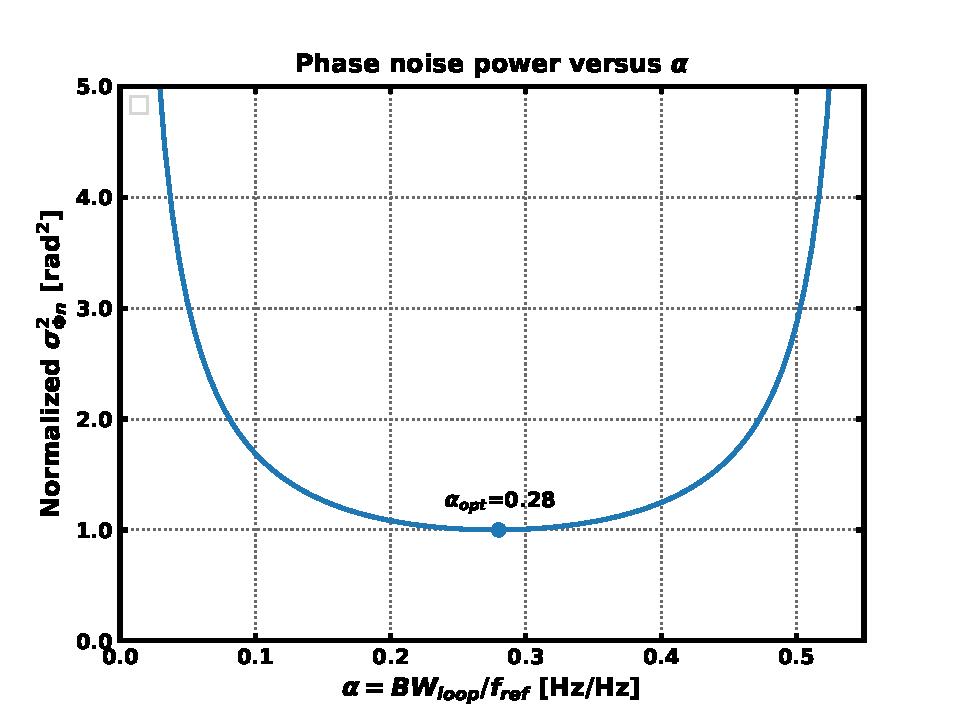
\includegraphics[width=0.6\textwidth, angle=0]{./figs/design/alpha_v_pn}
				\caption{Phase noise power (normalized) versus $\alpha$.}
				\label{fig:alpha_v_pn}
			\end{figure}

			It is possible to derive a constraint for BBPD jitter $\sigma^2_{\phi_j}$ in terms of $\alpha$ and a target $\sigma^2_{\phi_n}$ (i.e. CNR value), which allows for the performance specification for the physical BBPD to be set. Equation \ref{eq:bbpd_jit_pn} defines the maximum allowable phase noise power due to BBPD jitter, and equation \ref{eq:bbpd_t_jit_rms} defines the maximum RMS timing jitter of the same detector. In the case of 2.448 GHz operation, with 20 dB of CNR, and $\alpha$ = 0.1, the maximum allowable RMS BBPD jitter is $\sigma_{t_j}$ = 4.75 ps.
			\begin{equation}\label{eq:bbpd_jit_pn}
				\sigma^2_{\phi_j} \leq \sigma^2_{\phi_n}\left[\frac{4\sqrt{3+\sqrt{10}}}{5\pi^2\alpha} +\frac{2}{\pi} - 1 \right] - \frac{2S_{0_{osc}}(3 + \sqrt{10})}{5\pi\alpha^2f_{ref}}
			\end{equation}
			\begin{equation}\label{eq:bbpd_t_jit_rms}
				\sigma_{t_j} \leq \frac{1}{2\pi f_{osc}}\sqrt{\sigma^2_{\phi_n}\left[\frac{4\sqrt{3+\sqrt{10}}}{5\pi^2\alpha} +\frac{2}{\pi} - 1 \right] - \frac{2S_{0_{osc}}(3 + \sqrt{10})}{5\pi\alpha^2f_{ref}}}
			\end{equation}

			Now with theory in place to optimize PLL performance, mapping of the optimal parameter $K$ onto the loop filter of equation \ref{eq:pi_pll_tf} will be considered. Recall that $\omega_z = K_i/K_p = \sqrt{K}/2\zeta$ and $K = 2\pi K_{BBPD}K_{DCO}K_{i}$. The parameters $K_i$, $K_p$, and $\omega_z$ are thus provided in equations \ref{eq:wz_}-\ref{eq:ki_}.
			\begin{align}
				\omega_z &= \frac{\sqrt{K}}{2}\label{eq:wz_}\\
				K_p &= \frac{\sqrt{K}}{\pi K_{BBPD}K_{DCO}} = \frac{\sqrt{K}\sqrt{\sigma^2_{\phi_j} + \sigma^2_{\phi_n}}}{\sqrt{2\pi}K_{DCO}}\\
				K_i &= \frac{K}{2\pi K_{BBPD}K_{DCO}} = \frac{K\sqrt{\sigma^2_{\phi_j} + \sigma^2_{\phi_n}}}{2\sqrt{2\pi}K_{DCO}}\label{eq:ki_}
			\end{align}
	
	\FloatBarrier
	\subsubsection{Settling Time}
		If $\zeta$ is constrained to $\leq 1$:
		\begin{equation}
			\tau = \frac{1}{|\min(\Re(\{s_{p1}, s_{p2}\}))|} = \frac{1}{\zeta\sqrt{K}}
		\end{equation}
		Thus settling time is:
		\begin{equation}
			t_s = \frac{-\ln(\delta)}{\zeta\sqrt{K}} = \frac{-\ln\left(\frac{f_{tol}}{|f_i - Nf_{ref}|}\right)}{\zeta\sqrt{K}} 
		\end{equation}

		\subsubsection{Filter Design for Synchronous counter}
			\hl{WIP}
			Use fixed damping=1, maximize loop bandwidth, use Kpd of synchronous counter. Estimate settling time. 

		\subsubsection{PI-controller phase margin}\label{pi_phase_margin}
			The PI-PLL architecture of this work has a phase margin determined by the damping ratio $\zeta$, given by equation \ref{eq:pm_pi_pll}. Figure \ref{fig:phase_margin} shows phase margin versus $0 \geq \zeta \geq 1$ of the PI-controller PLL. It is recommended to use at least 30-60 degrees in phase margin to achieve stability \cite{ogata_2010_stability}. In this work, $\zeta$ = 1 has been used, so a phase margin of 76 degrees is expected, and accordingly stability should be expected.
			\begin{equation}\label{eq:pm_pi_pll}
				\angle \text{L}(\omega_{ug}) = \frac{180}{2\pi}\arctan\left(2\zeta\sqrt{2\zeta^2 + \sqrt{4\zeta^4+1}}\right)\hspace{1em}[\text{degrees}]
			\end{equation}
			\begin{figure}[htb!]
				\center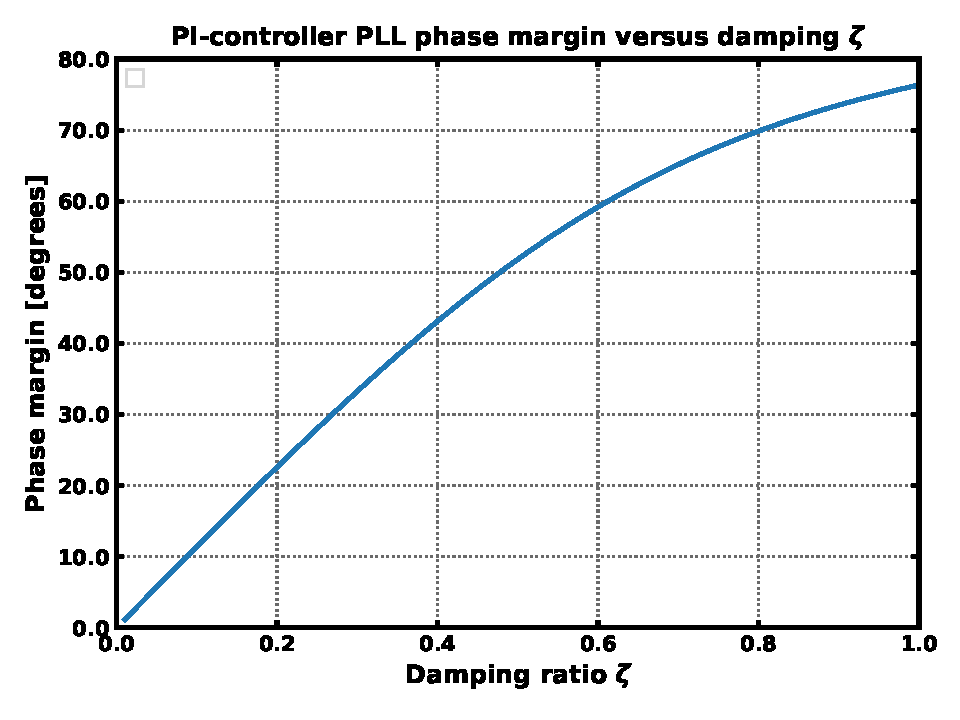
\includegraphics[width=0.5\textwidth, angle=0]{figs/damping_vs_pm.pdf}
				\caption{PI-controller PLL phase margin versus damping ratio.}
				\label{fig:phase_margin}
			\end{figure}



	\subsubsection{Discretization of Loop Filter}\label{disc_lf_comp_pi}
		Using the continuous filter discretization approach described in section \ref{lf-discretization} on the loop filter of equation \ref{eq:pi_pll_tf} results in equation \ref{eq:z_lf}.
		\begin{align}
			\textnormal{H}_{LF}(z) & = \left.\frac{K_i}{s}\left(\frac{s}{\omega_z} + 1\right)\right\vert_{s=\frac{1}{\Delta T_s}(1-z^{-1})}
			&= K_p\frac{(1+\omega_z\Delta T_s)-z^{-1}}{1- z^{-2}}\label{eq:z_lf}
		\end{align}

		The transformation of equation \ref{eq:z_lf} into a digitally implementable design as a direct form 1 IIR filter shown in figure \ref{fig:filt_imple}. Its filter coefficients given by equations \ref{eq:b0} and \ref{eq:b1}.
		\begin{figure}[htb!]
			\center\fontfamily{\sfdefault}\selectfont
% XCircuit output "filter_arch_pi.tex" for LaTeX input from filter_arch_pi.ps
\def\putbox#1#2#3#4{\makebox[0.00000in][l]{\makebox[#1][l]{}\raisebox{\baselineskip}[0.00000in][0.00000in]{\raisebox{#2}[0.00000in][0.00000in]{\scalebox{#3}{#4}}}}}
\def\rightbox#1{\makebox[0.00000in][r]{#1}}
\def\centbox#1{\makebox[0.00000in]{#1}}
\def\topbox#1{\raisebox{-0.60\baselineskip}[0.00000in][0.00000in]{#1}}
\def\midbox#1{\raisebox{-0.20\baselineskip}[0.00000in][0.00000in]{#1}}
   \scalebox{1}{
   \normalsize
   \parbox{5.54167in}{
   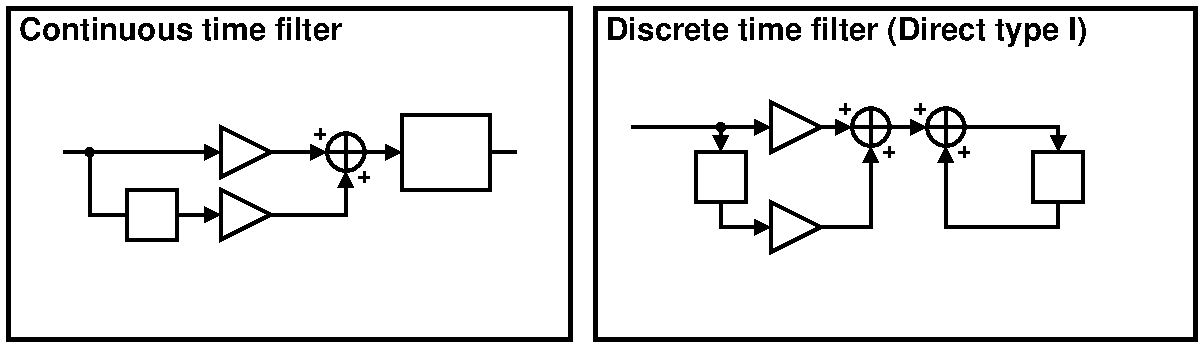
\includegraphics[scale=0.70000]{./figs/filter_arch_pi.pdf}\\
   % translate x=1728 y=944 scale 0.38
   \putbox{1.91800in}{0.90300in}{0.96}{$\frac{1}{\frac{s}{\omega_p} + 1}$}%
   \putbox{1.14800in}{1.01500in}{0.96}{$K_p$}%
   \putbox{1.14800in}{0.72800in}{0.96}{$K_i$}%
   \putbox{0.60900in}{0.58100in}{0.96}{$1/s$}%
   \putbox{0.25900in}{0.98700in}{0.96}{x[n]}%
   \putbox{2.35900in}{0.98700in}{0.96}{y[n]}%
   \putbox{2.92600in}{1.10600in}{0.96}{x[n]}%
   \putbox{4.99800in}{1.01500in}{0.96}{\rotatebox{-360}{y[n]}}%
   \putbox{3.26200in}{0.75600in}{0.96}{$z^{-1}$}%
   \putbox{3.73100in}{1.13400in}{0.96}{b$_0$}%
   \putbox{3.73100in}{0.66500in}{0.96}{b$_1$}%
   \putbox{4.83700in}{0.75600in}{0.96}{$z^{-1}$}%
   \putbox{4.99800in}{0.55300in}{0.96}{y[n-1]}%
   } % close 'parbox'
   } % close 'scalebox'
   \vspace{-\baselineskip} % this is not necessary, but looks better
\fontfamily{\rmdefault}\selectfont

			\caption{Implementation of filter.}
			\label{fig:filt_imple}
		\end{figure}
					% y[n] = x[n]\frac{K_i\omega_pT}{\omega_z}\frac{1+\omega_zT}{1+\omega_pT} - x[n-1]\frac{K_i\omega_pT}{\omega_z}\frac{1}{1+\omega_pT} + y[n-1]\frac{2+\omega_pT}{1+\omega_pT} - y[n-2]\frac{1}{1+\omega_pT}\\
					% = a_0x[n] + a_1x[n-1] - b_1y[n-1] - b_2x[n-2] 
		\begin{align}
			b_0 &= K_p (1+\omega_z\Delta T_s)=\frac{\sqrt{K}\sqrt{\sigma^2_{\phi_j} + \sigma^2_{\phi_n}}}{\sqrt{2\pi}K_{DCO}}\left(1+\frac{\sqrt{K}}{2f_{ref}}\right)\label{eq:b0}\\
			 b_1 &= -K_p = - \frac{\sqrt{K}\sqrt{\sigma^2_{\phi_j} + \sigma^2_{\phi_n}}}{\sqrt{2\pi}K_{DCO}}\label{eq:b1}
		\end{align}
		If design of the PLL is with fixed target for $\sigma^2_{\phi_n}$ (CNR), has a known $\sigma^2_{\phi_j}$ for the BBPD, and $\alpha$ is selected to be constant (i.e. 0.1), the filter coefficients may be calculated as in equations \ref{eq:b0_} and \ref{eq:b1_}.

		\begin{align}
			b_0 &= \frac{\alpha f_{ref}\sqrt{2\pi}\sqrt{\sigma^2_{\phi_j} + \sigma^2_{\phi_n}}}{\sqrt{3+\sqrt{10}}K_{DCO}} \left(1+\frac{\pi\alpha}{\sqrt{3+\sqrt{10}}}\right)\label{eq:b0_}\\
			 b_1 &= - \frac{\alpha f_{ref}\sqrt{2\pi}\sqrt{\sigma^2_{\phi_j} + \sigma^2_{\phi_n}}}{\sqrt{3+\sqrt{10}}K_{DCO}}\label{eq:b1_}
		\end{align}
		%%%%




		\subsubsection{Implementation}
			The filter has been chosen to be implemented with separate parts to implement the feedforward parts for each phase detector of the PI-controller, but with a common integrator at the output, as shown in figure \ref{fig:pi_dig_imp}. This approach to reduce power in steady state operation (using the BBPD). The rationale is that the synchronous counter is a linear detector, thus requires multipliers in the datapath to implement the filter, whereas the BBPD only outputs two values, so the multipliers can be replaces with multiplexers that select between two products ($\pm b_0$ and $\pm b_1$) depending on the input. It is lower energy to operate a multiplexer than an array multiplier due to substantially lower complexity of logic, so the usage of two multiplexers in steady to implement the multipliers will result in substantial power savings. The usage of a common integrator used in both detector modes allows for continuity of output stage during transition between detector modes. 

			\begin{figure}[htb!]
			        \centering
			        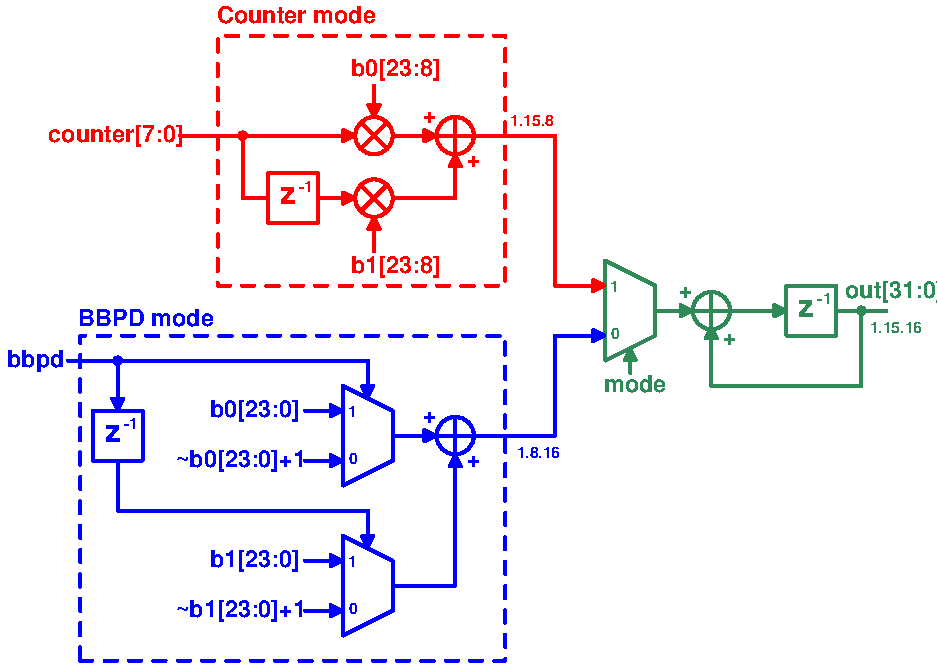
\includegraphics[width=0.75\textwidth, angle=0]{./figs/mux_datapath}
			    \caption{PI-controller implementation for combination of BBPD and synchronous counter usage.}
			    \label{fig:pi_dig_imp}
			\end{figure}

%%%%%%%%%%%%%%%%%%%%%%%%%%%%%%%%%%%%%%%%%%%%%
% \pagebreak
% \section{phase noise components....}

% 	\begin{figure}[htb!]
% 	    \centering
% 	    \begin{subfigure}{0.5\textwidth}
% 	        \centering
% 	        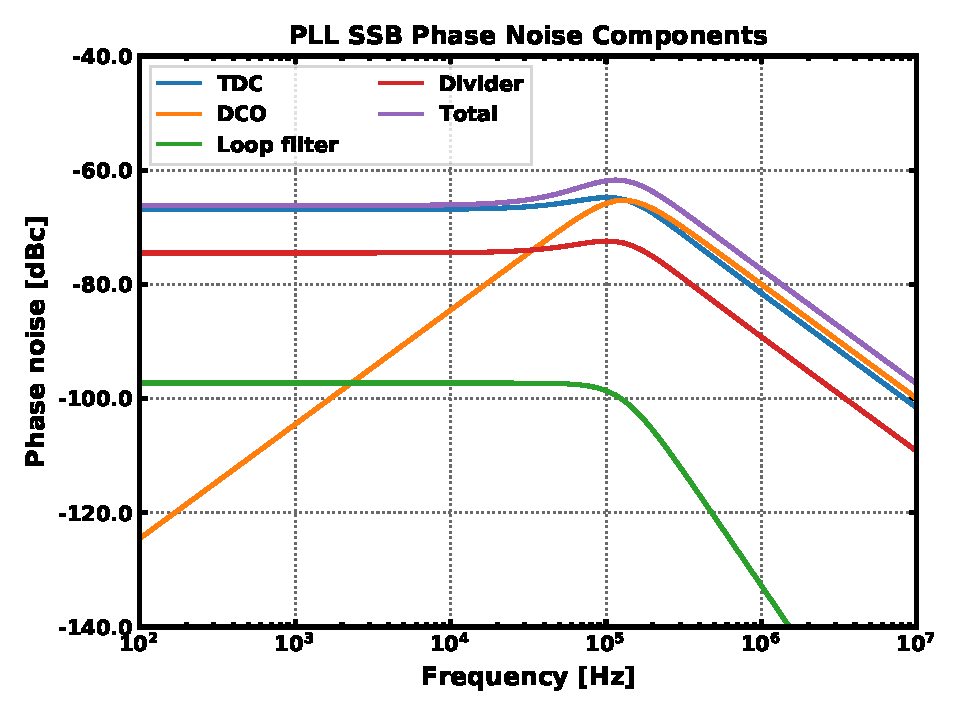
\includegraphics[width=1\textwidth, angle=0]{figs/pn_comps.pdf}
% 	        \caption{ }
% 	        \label{fig:ex_pll_pn_comps}
% 	    \end{subfigure}%
% 	    \begin{subfigure}{0.5\textwidth}
% 	        \centering
% 	        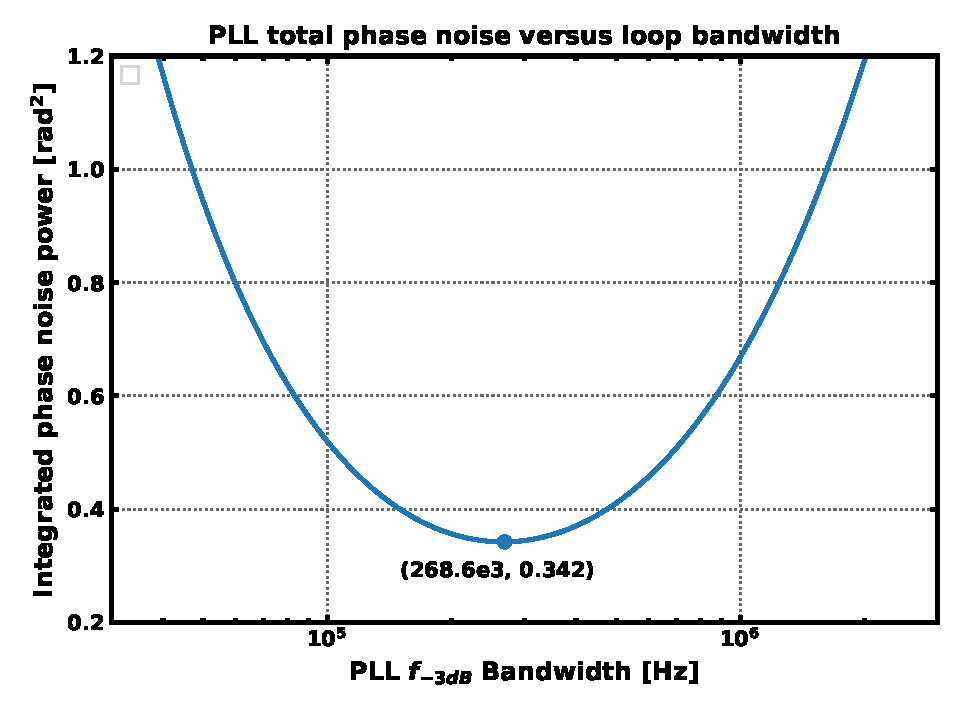
\includegraphics[width=1\textwidth, angle=0]{figs/bandwidth_vs_pn.pdf}
% 	        \caption{ }
% 	        \label{fig:bw_pn_tradeoff}
% 	    \end{subfigure}
% 	    % \caption{Approximate model for ring oscillator inverter delay cell.}
% 	    \label{fig:pll_pn_examples}
% 	    \caption{\textbf{(a)} Example PLL phase noise from models in this work, \textbf{(b)} integrated phase noise power versus bandwidth for the same PLL.}
% 	\end{figure}

% \begin{figure}[htb!]
% 	\center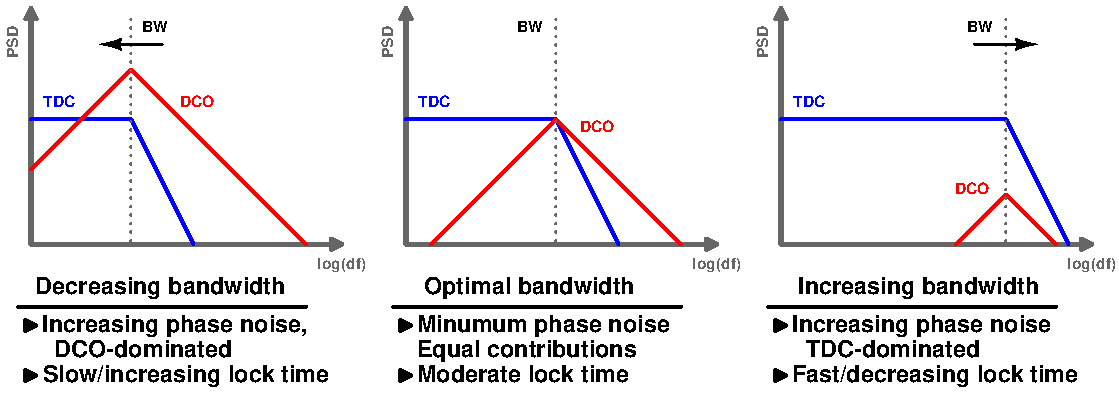
\includegraphics[width=1\textwidth, angle=0]{figs/loop_bandwidth}
% 	\caption{Bandwidth versus total integrated phase noise of PLL.}
% 	\label{fig:bw_vs_pn2}
% \end{figure}



\subsubsection{Loop Filter Quantization Noise Optimization}\label{lf_quant_noise_opt}


	\begin{figure}[htb!]
	    \centering
	    \begin{subfigure}{0.5\textwidth}
	        \centering
	        \center\fontfamily{\sfdefault}\selectfont
% XCircuit output "lf_quant_noise_model.tex" for LaTeX input from lf_quant_noise_model.ps
\def\putbox#1#2#3#4{\makebox[0.00000in][l]{\makebox[#1][l]{}\raisebox{\baselineskip}[0.00000in][0.00000in]{\raisebox{#2}[0.00000in][0.00000in]{\scalebox{#3}{#4}}}}}
\def\rightbox#1{\makebox[0.00000in][r]{#1}}
\def\centbox#1{\makebox[0.00000in]{#1}}
\def\topbox#1{\raisebox{-0.60\baselineskip}[0.00000in][0.00000in]{#1}}
\def\midbox#1{\raisebox{-0.20\baselineskip}[0.00000in][0.00000in]{#1}}
   \scalebox{1}{
   \normalsize
   \parbox{2.33750in}{
   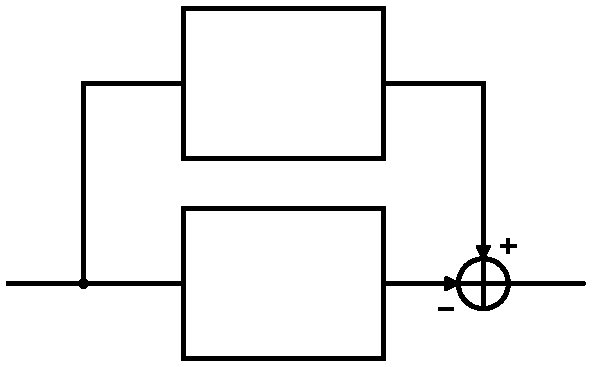
\includegraphics[scale=0.60000]{./figs/lf_quant_noise_model.pdf}\\
   % translate x=448 y=448 scale 0.38
   \putbox{0.93600in}{1.08600in}{0.96}{$\text{H}_{LF}$(z)}%
   \putbox{0.93600in}{0.43200in}{0.96}{$\hat{\text{H}}_{LF}$(z)}%
   \putbox{0.98400in}{0.28200in}{0.84}{(B-bit}%
   \putbox{0.88200in}{0.13200in}{0.84}{quantized)}%
   \putbox{0.06000in}{0.43200in}{0.96}{w[n]}%
   \putbox{2.08200in}{0.43200in}{0.96}{q[n]}%
   \putbox{1.58400in}{1.23600in}{0.96}{y[n]}%
   \putbox{1.58400in}{0.43200in}{0.96}{$\hat{\text{y}}$[n]}%
   } % close 'parbox'
   } % close 'scalebox'
   \vspace{-\baselineskip} % this is not necessary, but looks better
\fontfamily{\rmdefault}\selectfont

	        \caption{ }
	        \label{fig:lf_quant_noise_model}
	    \end{subfigure}%
	    \begin{subfigure}{0.5\textwidth}
	        \centering
	       \center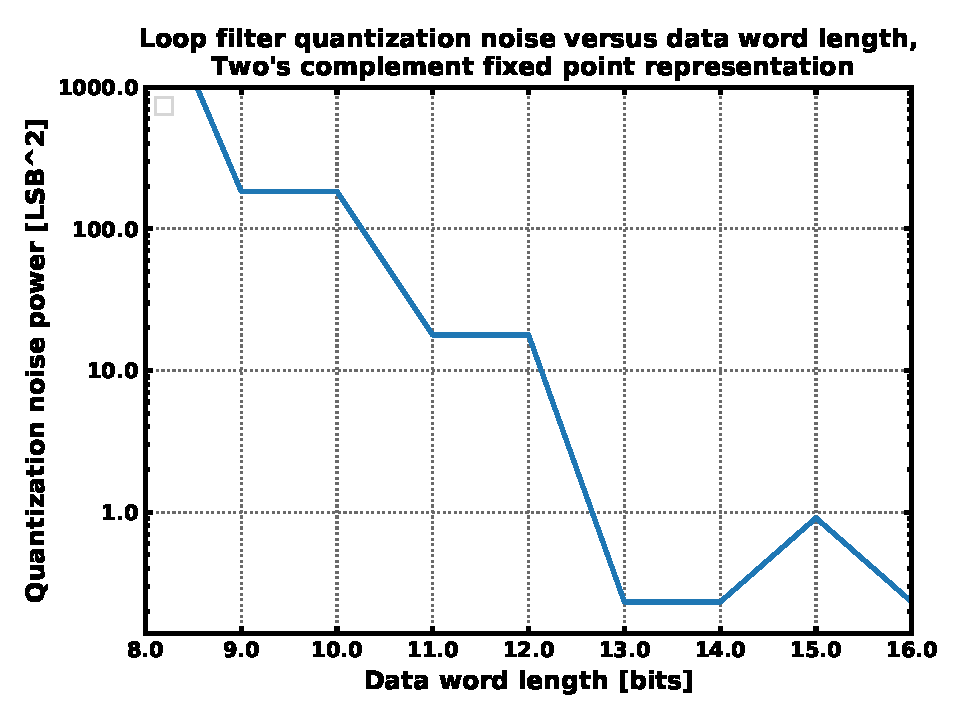
\includegraphics[width=1\textwidth, angle=0]{figs/lf_quant_noise.pdf}
	        \caption{ }
	        \label{fig:lf_quant_mse}
	    \end{subfigure}
	    % \caption{Approximate model for ring oscillator inverter delay cell.}
	    \label{fig:lf_quant_noise_opt}
	    \caption{\textbf{(a)} Model for determining quantization noise of loop filter, \textbf{(b)} Quantization noise power power out of an example loop filter versus data word resolution.}
	\end{figure}




% \begin{figure}[htb!]
% 	\center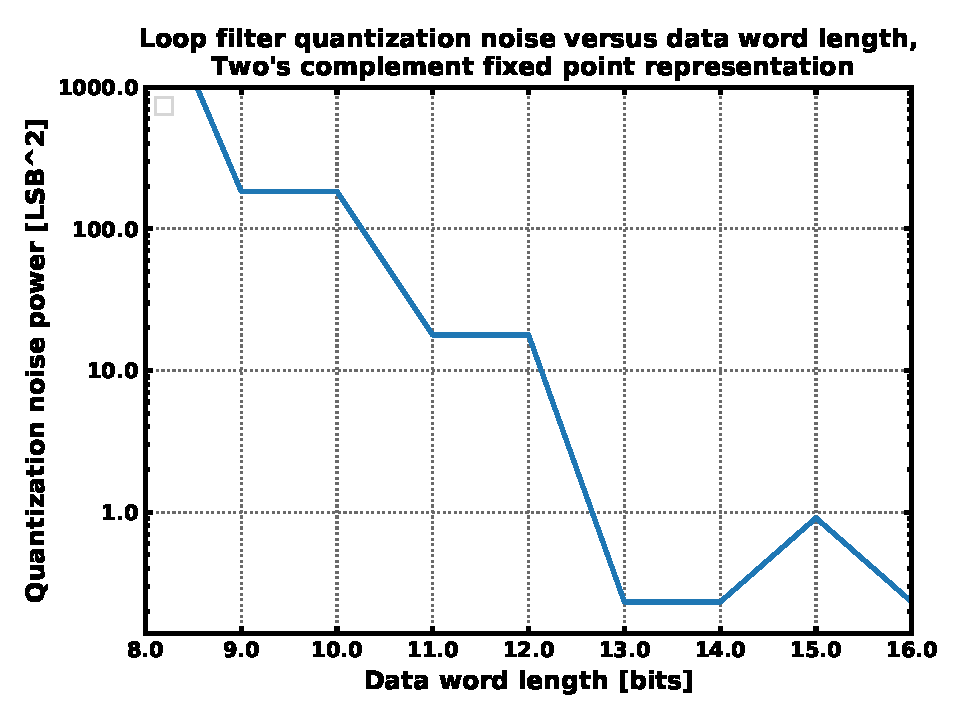
\includegraphics[width=0.5\textwidth, angle=0]{figs/lf_quant_noise.pdf}
% 	\caption{Quantization noise power power out of an example loop filter versus data word resolution.}
% 	\label{fig:lf_quant_mse}
% \end{figure}


\subsubsection{Loop Filter Transfer Function Error Optimization}

\begin{figure}[htb!]
    \centering
    \begin{subfigure}{0.5\textwidth}
        \centering
        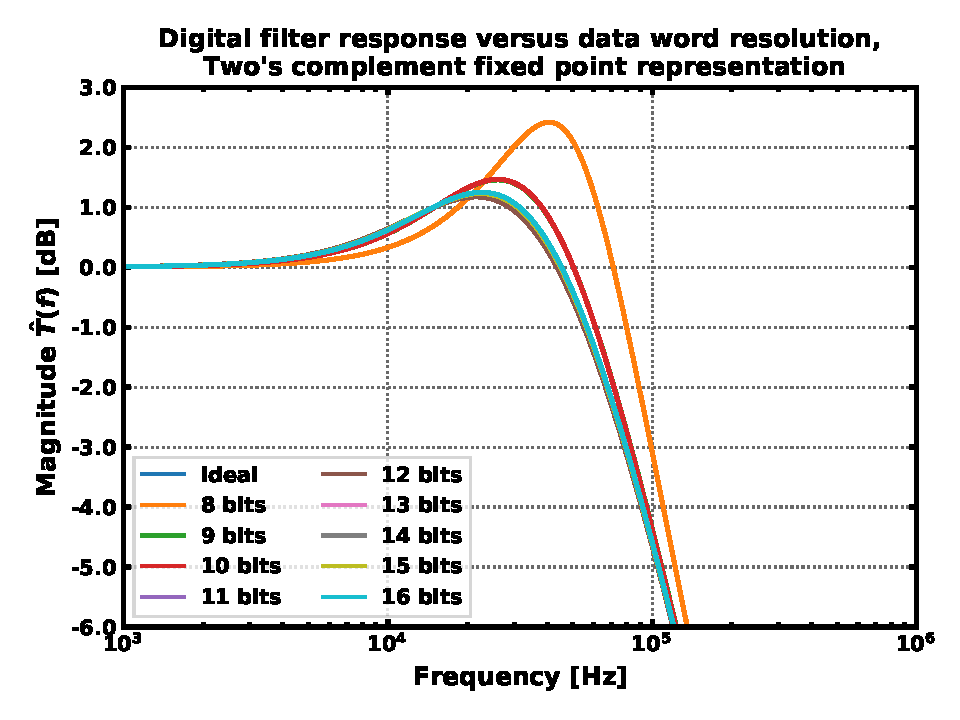
\includegraphics[width=1\textwidth, angle=0]{figs/tf_quant_error.pdf}
        \caption{ }
        \label{fig:tf_curves_quant_error}
    \end{subfigure}%
    \begin{subfigure}{0.5\textwidth}
        \centering
        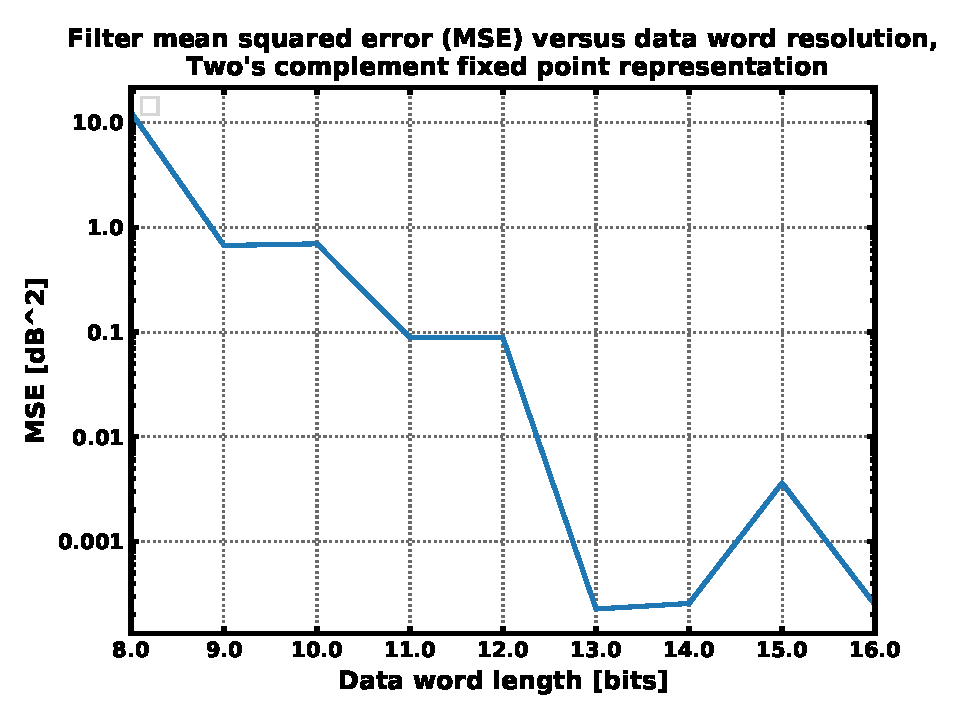
\includegraphics[width=1\textwidth, angle=0]{figs/tf_mse.pdf}
        \caption{ }
        \label{fig:tf_mse}
    \end{subfigure}
    % \caption{Approximate model for ring oscillator inverter delay cell.}
    \label{fig:tf_quant_error}
    \caption{\textbf{(a)} Example filter error due to coefficient quantization, \textbf{(b)} Example MSE error of filter design due to coefficient quantization.}
\end{figure}
\FloatBarrier






		\subsubsection{Approach 2: Results of Transient and Phase Noise Simulation}
		It is observed that the fast lock gear converges the PLL to steady state in approximately 6 $\mu$s as seen in the transient step simulation in figures \ref{fig:trans_lf_fast} and \ref{fig:trans_inst_freq_fast}, where an initial frequency error of 0.5\% {12 MHz} is used. Figure \ref{fig:trans_det_fast} shows the output of the TDC and BBPD, it is seen that BBPD feedback has a high density at approximately 11 $\mu$s, implicating steady state conditions. Finally, the computed phase noise spectrum of figure \ref{fig:trans_phase_noise_fast} demonstrates that there is some discrepancy between the ideal designed response and that simulated, albeit the bandwidth appears correct. The phase noise spectrum discrepancy is likely due to the model used in the optimization for the BBPD, which uses a linearized model of the BBPD with only idealized DCO and detector noise considered. This does not accurately account for all quantization and discretization emergent behaviors in the discrete time behavioral simulation possibly being manifested here. 

			\begin{figure}[htb!]
			    \centering
			    \begin{subfigure}{0.5\textwidth}
			        \centering
			        \center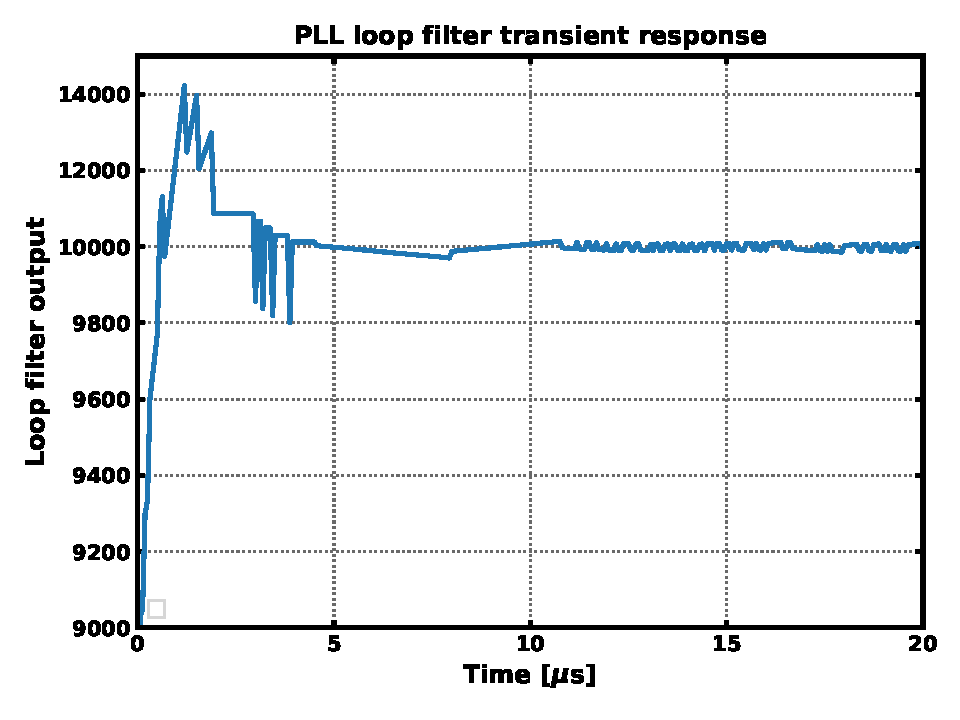
\includegraphics[width=1.0\textwidth, angle=0]{figs/trans_loop_filter_fast.pdf}
			        \caption{ }
			        \label{fig:trans_lf_fast}
			    \end{subfigure}%
			    \begin{subfigure}{0.5\textwidth}
			        \centering
			        \center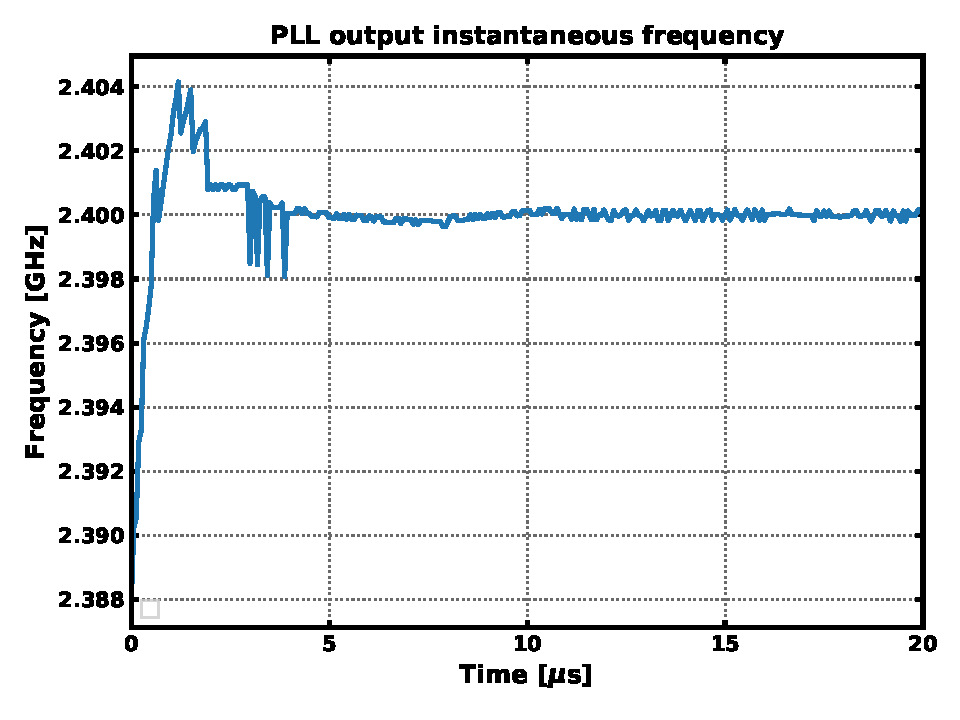
\includegraphics[width=1.0\textwidth, angle=0]{figs/trans_inst_freq_fast.pdf}
			        \caption{ }
			        \label{fig:trans_inst_freq_fast}
			    \end{subfigure}
			    % \caption{Approximate model for ring oscillator inverter delay cell.}
			    \label{fig:trans_sim1_fast}
			    \caption{Simulation with 0.5\% initial frequency error: \textbf{(a)} Loop filter transient response, \textbf{(b)} PLL output instantaneous frequency.}
			\end{figure}

			\begin{figure}[htb!]
			    \centering
			    \begin{subfigure}{0.5\textwidth}
			        \centering
			        \center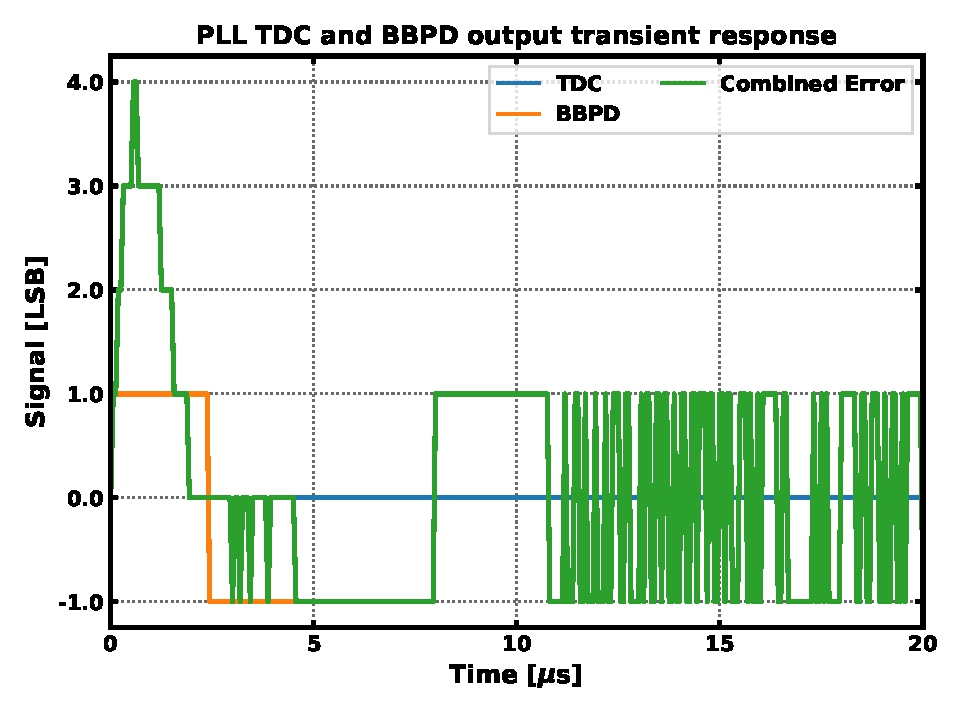
\includegraphics[width=1.0\textwidth, angle=0]{figs/trans_tdc_bbpd_fast.pdf}
			        \caption{ }
			        \label{fig:trans_det_fast}
			    \end{subfigure}%
			    \begin{subfigure}{0.5\textwidth}
			        \centering
			        \center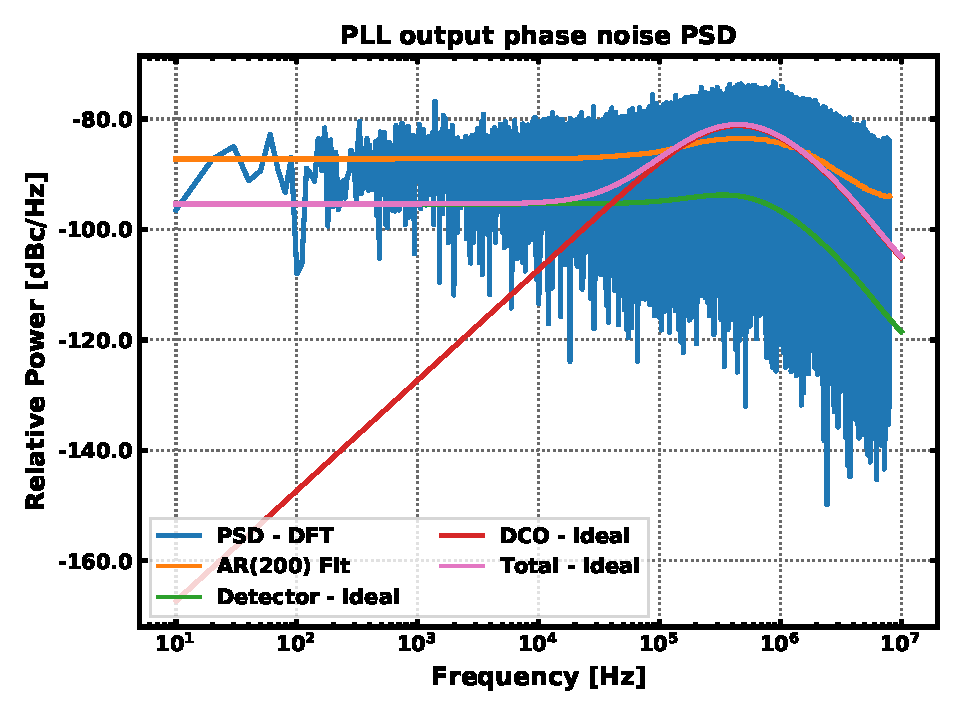
\includegraphics[width=1.0\textwidth, angle=0]{figs/trans_phase_noise_fast.pdf}
			        \caption{ }
			        \label{fig:trans_phase_noise_fast}
			    \end{subfigure}
			    % \caption{Approximate model for ring oscillator inverter delay cell.}
			    \label{fig:trans_sim2_fast}
			    \caption{Simulation with 12 MHz (0.5\%) initial frequency error: \textbf{(a)} BBPD/TDC detector responses, \textbf{(b)} PLL output phase noise power spectrum.}
			\end{figure}
		\subsubsection{Approach 2: Results of Parameter Sweep and Variational Analysis}
		The same parameter sweeps for $K_{DCO}$ and initial frequency error of approach 1 were applied here. In figures \ref{fig:sweep_kdco_fast} and \ref{fig:sweep_finit_fast}, the results of these sweeps are shown. The loop filter gear switching mechanism as modeled in the simulation waits a fixed time interval before switching gears, in this case chosen to be 2.0 times the estimated lock time given in table \ref{filter_params_fast_lock}. This interval has provided sufficient settling within the simulated parameter range of $K_{DCO}$ and initial frequency error that lock time stability is observed under most conditions, except under high offset for $K_{DCO}$ and initial frequency error. It was established for this simulation results that tolerance range for $K_{DCO}$ is -6950/+9750 Hz/LSB from the nominal 10000 Hz/LSB value, and the capture range is 168 MHz. Figures \ref{fig:mc_trans_fast} and \ref{fig:mc_hist_fast} demonstrate a variational simulation of the PLL using Monte-Carlo sampling, with 1000 samples. The simulation was configured to vary $K_{DCO}$ with a standard deviation of 20 \% of the nominal value, and to vary the initial starting frequency with a standard deviation of 60 MHz (2.5 \% of the final frequency). It was observed that the PLL stably locked for all simulation instances, a mean lock time of 5.96 $\mu$s was achieved. This value correlates well with the estimate of 5.52 $\mu$s from the filter design process. The upper bound for a 99\% confidence interval of lock time is 11.625 $\mu$s, thus meeting the 25$\mu$s lock time specification with considerable margin. The extracted PLL performance parameters from these simulations of this gear-switching PLL is in table \ref{simulation_params_fast}. 
			\begin{figure}[htb!]
			    \centering
			    \begin{subfigure}{0.5\textwidth}
			        \centering
			        \center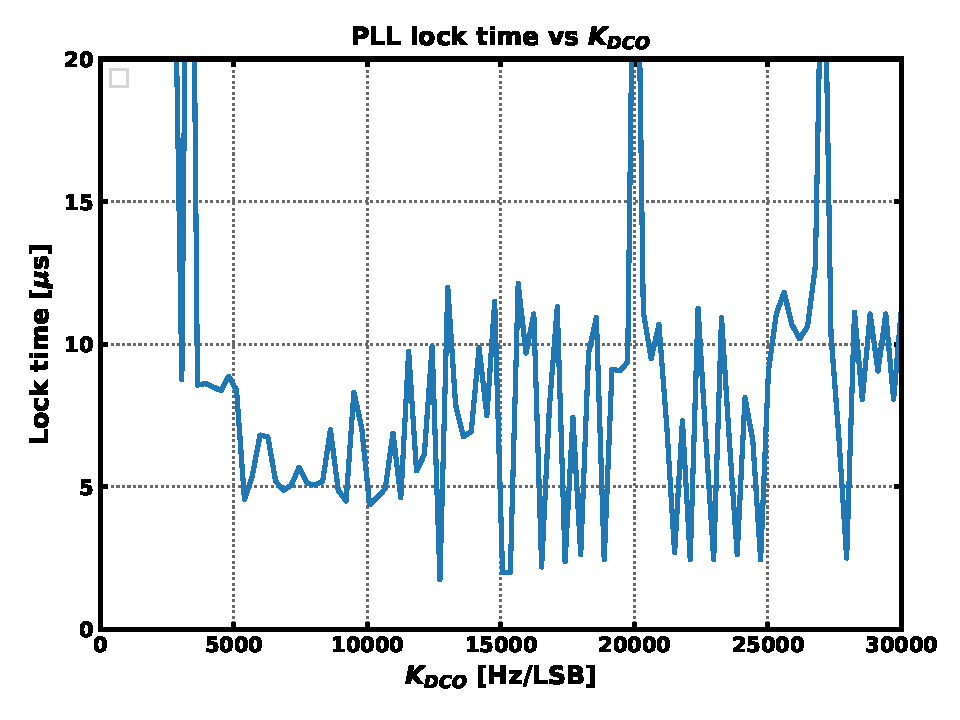
\includegraphics[width=1.0\textwidth, angle=0]{figs/_kdco_sweep_fast.pdf}
			        \caption{ }
			        \label{fig:sweep_kdco_fast}
			    \end{subfigure}%
			    \begin{subfigure}{0.5\textwidth}
			        \centering
			        \center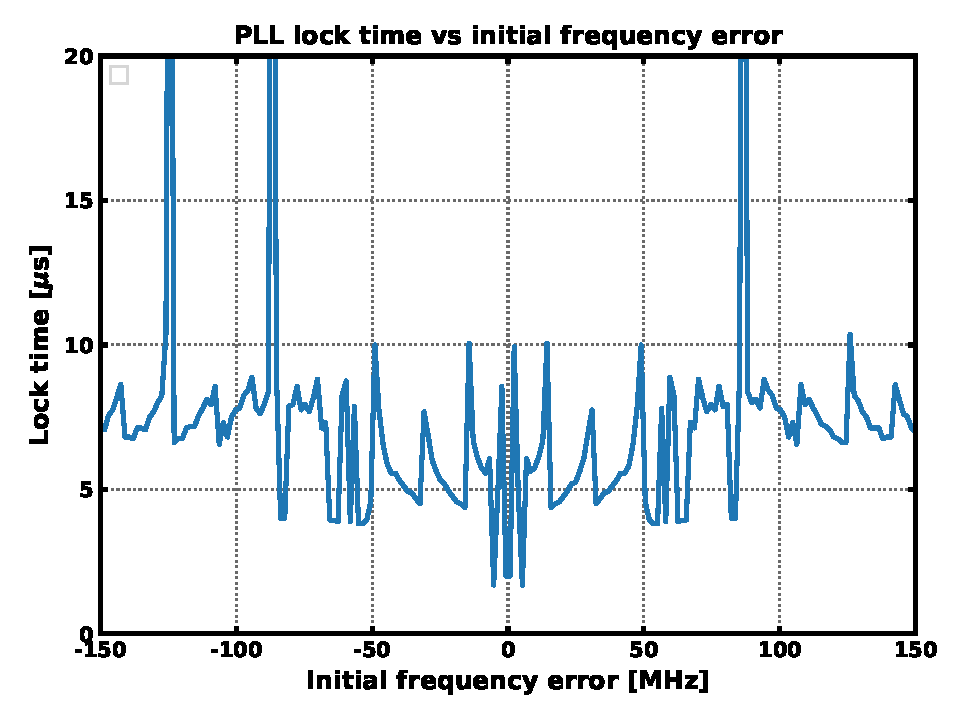
\includegraphics[width=1.0\textwidth, angle=0]{figs/finit_sweep_fast.pdf}
			        \caption{ }
			        \label{fig:sweep_finit_fast}
			    \end{subfigure}
			    % \caption{Approximate model for ring oscillator inverter delay cell.}
			    \label{fig:sweep_sim_fast}
			    \caption{\textbf{(a)} PLL lock time simulation with KDCO swept, 12 MHz (0.5\%) initial frequency error, \textbf{(b)} PLL lock time simulation with initial frequency error swept.}
			\end{figure}

			\begin{figure}[htb!]
			    \centering
			    \begin{subfigure}{0.5\textwidth}
			        \centering
			        \center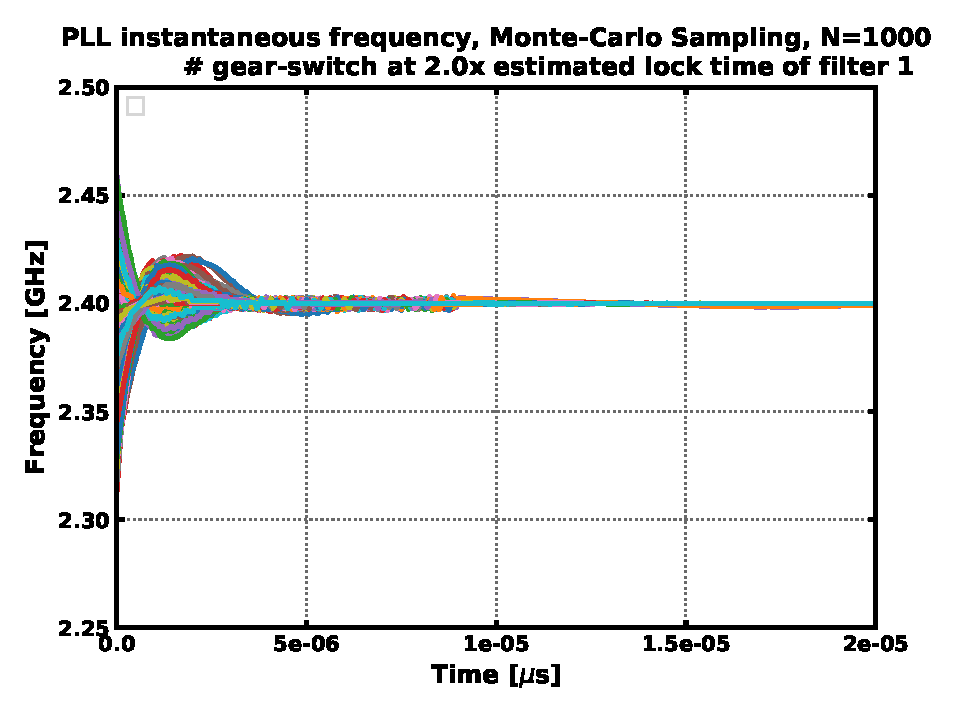
\includegraphics[width=1.0\textwidth, angle=0]{figs/mc_trans_2x.pdf}
			        \caption{ }
			        \label{fig:mc_trans_fast}
			    \end{subfigure}%
			    \begin{subfigure}{0.5\textwidth}
			        \centering
			        \center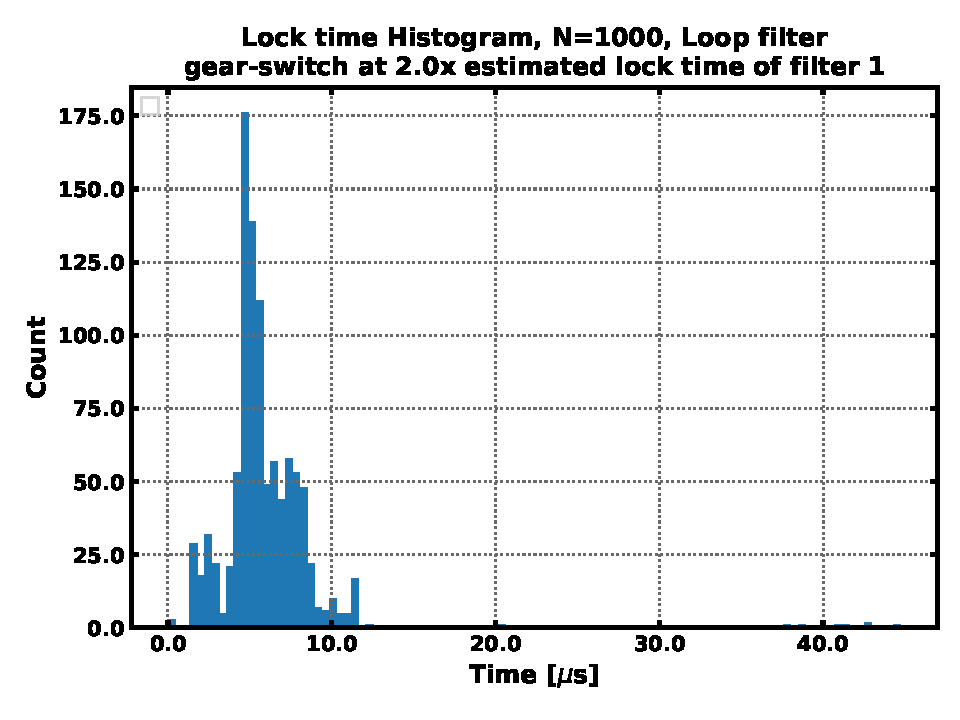
\includegraphics[width=1.0\textwidth, angle=0]{figs/mc_hist_fast_2x.pdf}
			        \caption{ }
			        \label{fig:mc_hist_fast}
			    \end{subfigure}
			    % \caption{Approximate model for ring oscillator inverter delay cell.}
			    \label{fig:mc_sim_fast}
			    \caption{Monte-Carlo simulation with 1000 samples, 20\% RMS deviation in KDCO, and 60 MHz (2.5\%) RMS deviation in initial frequency error \textbf{(a)} Frequency transient responses, \textbf{(b)} Lock time histogram.}
			\end{figure}

		\begin{table}[h!]
			\centering
			\def\arraystretch{1.5}		
			\setlength\arrayrulewidth{0.75pt}
			\setlength{\tabcolsep}{1em} % for the horizontal padding
			\begin{tabular}{|l|r|l|}
				\hline 
				\rule[-1ex]{0pt}{2.5ex} \cellcolor{gray!40}\textbf{Parameter} & \cellcolor{gray!40}\textbf{Value} & \cellcolor{gray!40}\textbf{Unit }\\ 
				\hline 
				\rule[-1ex]{0pt}{2.5ex} \textbf{$K_{DCO}$ Tolerance}  & -6950/+9750 & Hz/LSB \\
				\hline 
				\rule[-1ex]{0pt}{2.5ex} \textbf{Capture range}  & 168 ($\pm 84$)& MHz\\ 
				\hline 
				\rule[-1ex]{0pt}{2.5ex} \textbf{Mean lock time}  & 5.961688& $\mu$s \\
				\hline 
				\rule[-1ex]{0pt}{2.5ex} \textbf{Lock time $\sigma$} & 3.611130 & $\mu$s\\ 
				\hline 
				\rule[-1ex]{0pt}{2.5ex} \textbf{Lock time 99 \% CI upper bound} & 11.625  & $\mu$s\\
				\hline 
				\rule[-1ex]{0pt}{2.5ex} \textbf{Residual phase modulation} & $4.367535\times10^{-2}$ & rad$^2$\\ 
				\hline 
			\end{tabular} 

			% \caption{Assigned specifications for branch line hybrid design.}
			% \label{asgn_specs}
			\caption{PLL parameters extracted from variance and parameter sweep simulations.}
			\label{simulation_params_fast}
		\end{table}


		\subsubsection{Cyclostationary nonsense}


		\begin{figure}
			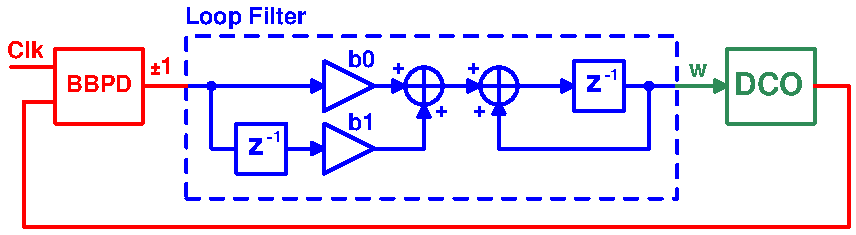
\includegraphics[width=0.8\textwidth, angle=0]{./figs/simplified_bbpll}
		\end{figure}
		\begin{itemize}[itemsep=4pt,label=\protect---]

			\item Output of BBPD is quantized $\pm$ 1. With PI loop filter architecture, there are only 4 possible values that the output {\color{teal}\textbf{w}} can increment by: $\lfloor b_0+b_1 \rfloor$, $\lfloor b_0-b_1 \rfloor$, $\lfloor -b_0+b_1 \rfloor$, $\lfloor -b_0-b_1 \rfloor$.
			\item In steady state, with the BBPD outputting a worst case sequence of +1/-1/+1/-1... , the output will toggle betwwen $\lfloor b_0-b_1 \rfloor$ and $\lfloor -b_0+b_1 \rfloor$.
			\begin{itemize}[itemsep=4pt,label=\protect$\bullet$]
				\item Current optimization yields $b_0$ = 8.899856, $b_1$ = -8.301153 
				\item Thus output {\color{teal}\textbf{w}} will increment by +17, -18, +17, -18 ...
				\item Essentially output will make large-ish jumps in frequency every reference cycle
			\end{itemize}
		\end{itemize}

	\begin{figure}[htb!]
	    \centering
	    \begin{subfigure}{0.5\textwidth}
	        \centering
	        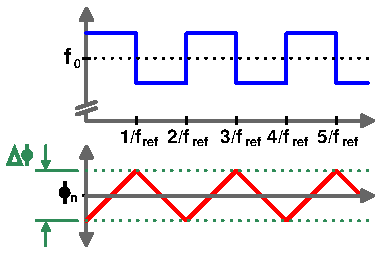
\includegraphics[width=0.8\textwidth, angle=0]{./figs/bbpd_resolution_phase_walk}
	    \end{subfigure}%
	    \begin{subfigure}{0.5\textwidth}
	        \centering
	        \center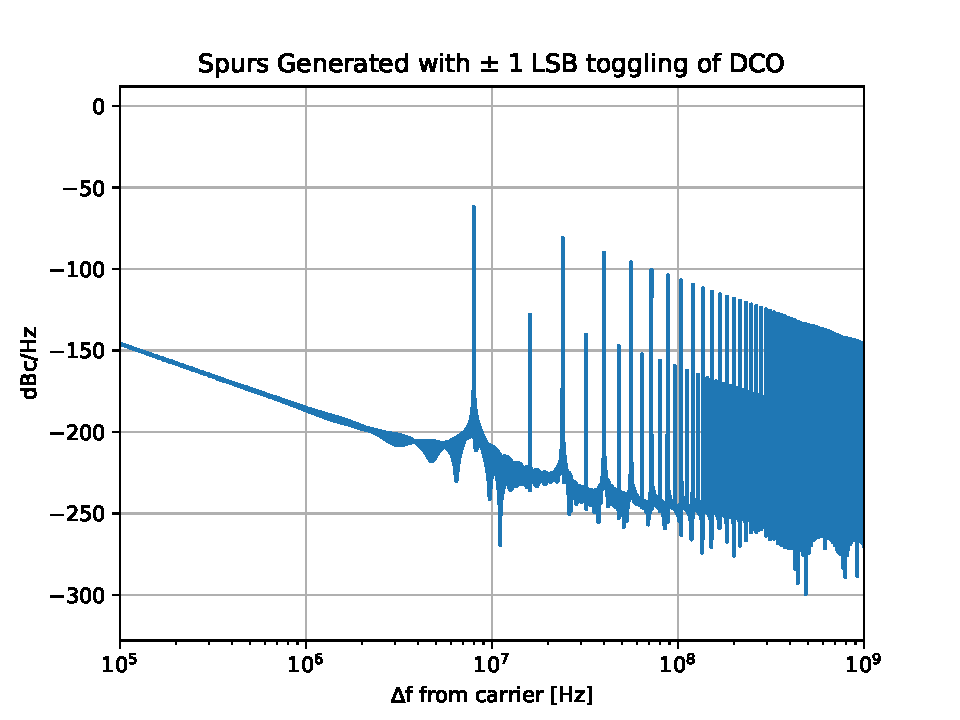
\includegraphics[width=0.8\textwidth, angle=0]{./figs/spurs_dco}
	    \end{subfigure}
	    % \caption{Approximate model for ring oscillator inverter delay cell.}
	\end{figure}
		\begin{itemize}[itemsep=4pt,label=\protect---]

			\item Worst case input sequence results in square wave frequency modulation, which in the phase domain creates a cyclostationary triangle wave with period $f_{ref}$/2. This creates \textbf{SPURS} at $f_{ref}$/2.
			\item In general, $f_{ref}$ $>>$ $K_{DCO}|b_0-b_1|$ (frequency deviation), so spurs are not generated at the deviation frequencies.
			\item With 1 LSB deviation per ref. cycle, a -62 dBc spur (SSB) is expected $f_{ref}$/2.
			\begin{itemize}[itemsep=4pt,label=\protect$\bullet$]
			\item Under my current $b_0$, $b_1$, this spur will be -37 dBc.
		\end{itemize}
		\end{itemize}



			% \vspace{100em}
			\begin{itemize}[itemsep=4pt,label=\protect---]
				\item \textbf{Cyclostationary (+1, -1, +1, -1, ...):}
				\begin{itemize}[itemsep=4pt,label=\protect$\bullet$]
					\item Under my system parameters, the total phase noise power from resolution effects is -34 dBc, essentially all of which is in the first spur at $f_{ref}/2$.
					\begin{equation}
						\Delta \Phi  = \frac{2\pi|b_0-b_1|K_{DCO}}{f_{ref}}
					\end{equation}
					\begin{equation}
						\sigma_{\Phi rj}  = \frac{\pi|b_0-b_1|K_{DCO}}{\sqrt{3}f_{ref}}
					\end{equation}
				\end{itemize}
			\item \textbf{General note:} the phase noise from this source must $<<$ than target SNR for PLL application. Can use these relations to find limits for maximum $K_{DCO}$ before resolution jitter is dominant.			
		\end{itemize}


			% \vspace{100em}
			\begin{itemize}[itemsep=4pt,label=\protect---]

				\item \textbf{Average case:}
				\begin{itemize}[itemsep=4pt,label=\protect$\bullet$]
					\item All transitions equally likely out of BBPD.
					\item Under my system parameters, the total phase noise power from resolution effects is -29.4 dBc (simulated).
					\item Phase noise is bimodal. The total RMS phase noise power is approximately equal to the absolute value of the distribution means.
					\begin{equation}
						\mu = \pm\frac{\pi|b_0-b_1|K_{DCO}}{f_{ref}}, \hspace{2em}\sigma_{\Phi rj} \approx |\mu|
					\end{equation}
				\end{itemize}
			\end{itemize}
	\vspace{-3em}
	\begin{figure}[htb!]
	    \centering
	    \begin{subfigure}{0.5\textwidth}
	        \centering
	        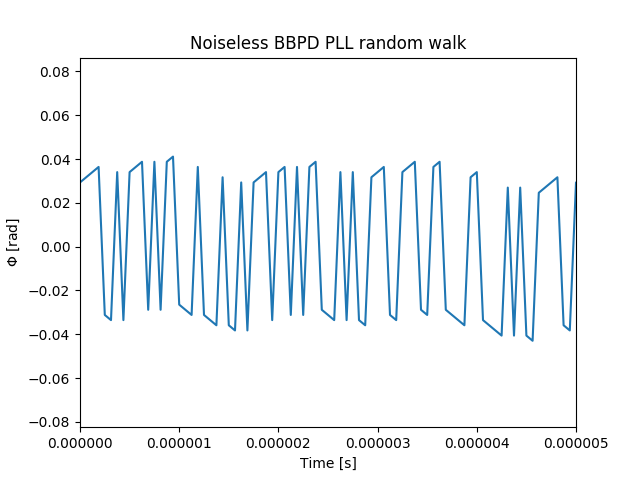
\includegraphics[width=0.8\textwidth, angle=0]{./figs/bbpd_rw}
	    \end{subfigure}%
	    \begin{subfigure}{0.5\textwidth}
	        \centering
	        \center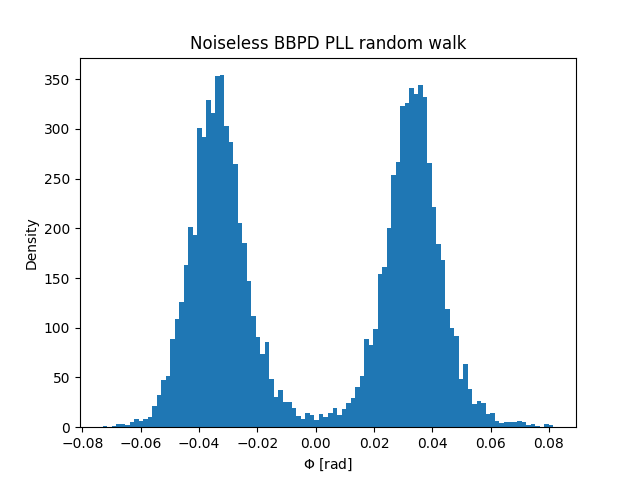
\includegraphics[width=0.8\textwidth, angle=0]{./figs/bbpd_rw_hist}
	    \end{subfigure}
	    % \caption{Approximate model for ring oscillator inverter delay cell.}
	\end{figure}



			% \vspace{100em}
			\begin{itemize}[itemsep=4pt,label=\protect---]
				\item Found an interesting dissertation on BBPD PLLs [3], which shows that the linearized BBPD gain model I have been using (K$_{BBPD}$ = $2/\sqrt{2\pi}\sigma_{\Phi_n}$) is not totally correct. 
				\begin{itemize}[itemsep=4pt,label=\protect$\bullet$]
						\item Due to BBPF-PLL resolution jitter, varies depending if resolution jitter or if random noise is the dominant component.
				\end{itemize}
				\item Need to account for this in my filter optimization code...
				\item An approximation, with random/uncorrelated noise with $\sigma_{\Phi uc}$, and resolution jitter $\sigma_{\Phi{rj}}$ (based on variable substitution of [3]'s theory):
				\begin{equation}
					K_{BBPD} = \frac{1}{\sqrt{2\pi}\sigma_{\Phi uc}}\left[1+ e^{-\frac{1}{2}\left(\frac{\sigma_{\Phi{rj}}}{\sigma_{\Phi uc}}\right)^2} \right]
				\end{equation}
					\begin{equation}
						\sigma_{\Phi rj} \approx \frac{\pi|b_0-b_1|K_{DCO}}{f_{ref}}
					\end{equation}
				\item Currently, I should be well into the random noise dominated regime.
			\end{itemize}

	
			\begin{figure}[htb!]
			        \centering
			        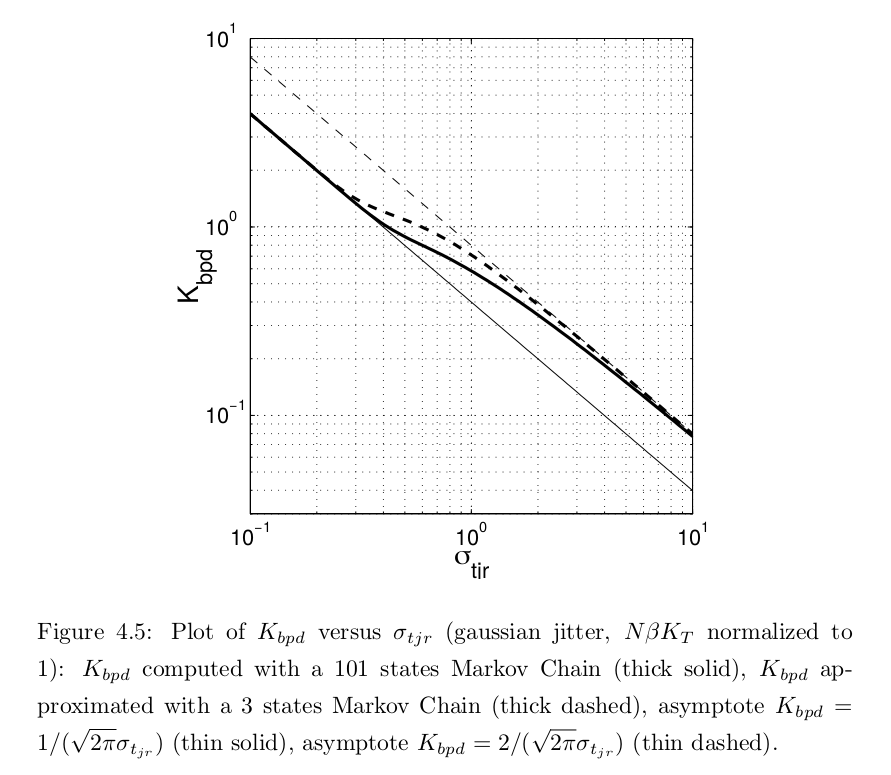
\includegraphics[width=1\textwidth, angle=0]{./figs/kbbpd}
			    % \caption{Approximate model for ring oscillator inverter delay cell.}
			\end{figure}

	\subsubsection{Filter Design}
		\begin{table}[h!]
			\centering
			\def\arraystretch{1.5}		
			\setlength\arrayrulewidth{0.75pt}
			\setlength{\tabcolsep}{1em} % for the horizontal padding
			\begin{tabular}{|l|r|l|}
				\hline 
				\rule[-1ex]{0pt}{2.5ex} \cellcolor{gray!40}\textbf{Parameter} & \cellcolor{gray!40}\textbf{Value} & \cellcolor{gray!40}\textbf{Unit }\\ 
				\hline 
				\rule[-1ex]{0pt}{2.5ex} \textbf{$K$}  & $2.982197\times10^{12}$ &  \\
				\hline 
				\rule[-1ex]{0pt}{2.5ex} \textbf{$K_i$}  & $2.982197\times10^{8}$ &  \\
				\hline 
				\rule[-1ex]{0pt}{2.5ex} \textbf{$K_p$}  & $2.115052\times10^{2}$ &  \\
				\hline 
				\rule[-1ex]{0pt}{2.5ex} \textbf{$f_z$} & $2.244064\times10^5$ & Hz\\
				\hline 
				\rule[-1ex]{0pt}{2.5ex} \textbf{$b_0$}  & $2.3014397180\times10^2$  &\\
				\hline 
				\rule[-1ex]{0pt}{2.5ex} \textbf{$b_1$}  & $-2.1150524223\times10^2$  & \\
				\hline 
				\rule[-1ex]{0pt}{2.5ex} \textbf{$a_0$}  & $1.0\times10^0$  &\\ 
				\hline 
				\rule[-1ex]{0pt}{2.5ex} \textbf{$a_1$}  & $-1.0\times10^0$  & \\
				\hline 
				\rule[-1ex]{0pt}{2.5ex} \textbf{$a_2$}  & $0.0\times10^0$  & \\
				\hline 
				\rule[-1ex]{0pt}{2.5ex} Estimated bandwidth & $5.333423\times10^5$ & Hz \\
				\hline 
				\rule[-1ex]{0pt}{2.5ex} Estimated lock time & $4.527067\times10^{-6}$ & seconds \\
				\hline 
			\end{tabular} 
			% \caption{Assigned specifications for branch line hybrid design.}
			% \label{asgn_specs}
			\caption{PLL parameters determined from filter design and optimization process for fast lock speed with TDC feedback.}
			\label{filter_params_fast_lock}
		\end{table}   

		\begin{table}[h!]
			\centering
			\def\arraystretch{1.5}		
			\setlength\arrayrulewidth{0.75pt}
			\setlength{\tabcolsep}{1em} % for the horizontal padding
			\begin{tabular}{|l|r|l|}
				\hline 
				\rule[-1ex]{0pt}{2.5ex} \cellcolor{gray!40}\textbf{Parameter} & \cellcolor{gray!40}\textbf{Value} & \cellcolor{gray!40}\textbf{Unit }\\ 
				\hline 
				\rule[-1ex]{0pt}{2.5ex} \textbf{$K$}  & $5.325862\times12^{12}$ &  \\
				\hline 
				\rule[-1ex]{0pt}{2.5ex} \textbf{$K_i$}  & $1.271456\times10^{10}$ &  \\
				\hline 
				\rule[-1ex]{0pt}{2.5ex} \textbf{$K_p$}  & $1.101813\times10^{4}$ &  \\
				\hline 
				\rule[-1ex]{0pt}{2.5ex} \textbf{$f_z$} & $1.836596\times10^5$ & Hz\\
				\hline 
				\rule[-1ex]{0pt}{2.5ex} \textbf{$b_0$}  & $1.1812790734\times10^4$  &\\
				\hline 
				\rule[-1ex]{0pt}{2.5ex} \textbf{$b_1$}  & $-1.1018130778\times10^4$  & \\
				\hline 
				\rule[-1ex]{0pt}{2.5ex} \textbf{$a_0$}  & $1.0\times10^0$  &\\ 
				\hline 
				\rule[-1ex]{0pt}{2.5ex} \textbf{$a_1$}  & $-1.0\times10^0$  & \\ 
				\hline 
				\rule[-1ex]{0pt}{2.5ex} \textbf{$a_2$}  & $0.0\times10^0$  & \\ 
				\hline 
				\rule[-1ex]{0pt}{2.5ex} \textbf{$K_{bb}$}  & $1.0\times10^0$  & \\ 
				\hline 
				\rule[-1ex]{0pt}{2.5ex} Estimated bandwidth & $9.117332\times10^5$ & Hz \\
				\hline 
				\rule[-1ex]{0pt}{2.5ex} Estimated lock time & $9.978130\times10^{-7}$ & seconds \\
				\hline 
			\end{tabular} 
			% \caption{Assigned specifications for branch line hybrid design.}
			% \label{asgn_specs}
			\caption{PLL parameters determined from filter design and optimization process for minimum phase noise with BBPD.}
			\label{filter_params_bbpd_low_noise}
		\end{table}   

		\begin{table}[h!]
			\centering
			\def\arraystretch{1.5}		
			\setlength\arrayrulewidth{0.75pt}
			\setlength{\tabcolsep}{1em} % for the horizontal padding
			\begin{tabular}{|l|r|r|l|}
				\hline 
				\rule[-1ex]{0pt}{2.5ex} \cellcolor{gray!40}\textbf{Parameter} & \cellcolor{gray!40}\textbf{Value} & \cellcolor{gray!40}\textbf{Value (digital) } & \cellcolor{gray!40}\textbf{Value Error}\\ 
				\hline 
				\rule[-1ex]{0pt}{2.5ex} Total dataword bits  & 20 & & \\ 
				\hline 
				\rule[-1ex]{0pt}{2.5ex} Sign bits  & 1 & & \\ 
				\hline 
				\rule[-1ex]{0pt}{2.5ex} Integer bits & 8 & & \\ 
				\hline 
				\rule[-1ex]{0pt}{2.5ex} Fractional bits  & 11 & & \\ 
				\hline 
				\rule[-1ex]{0pt}{2.5ex} \textbf{$b_0$} {\color{red} (gear 1)} & $2.301440\times10^2$ & \texttt{0b01110011000100100111}  & $+7.116930\times10^{-5}$\\
				\hline 
				\rule[-1ex]{0pt}{2.5ex} \textbf{$b_1$} {\color{red} (gear 1)} & $-2.115054\times10^2$ & \texttt{0b11110110001111110101}  & $-1.288619\times10^{-4}$\\
				\hline 
				\rule[-1ex]{0pt}{2.5ex} \textbf{$a_0$} {\color{red} (gear 1)} & $1.0\times10^0$ & \texttt{0b00000000100000000000} & $0.0\times10^0$ \\ 
				\hline 
				\rule[-1ex]{0pt}{2.5ex} \textbf{$a_1$} {\color{red} (gear 1)} & $-1.0\times10^0$ & \texttt{0b11111111100000000000} & $0.0\times10^0$ \\ 
				\hline 
				\rule[-1ex]{0pt}{2.5ex} \textbf{$a_2$} {\color{red} (gear 1)} & $0.0\times10^0$ & \texttt{0b00000000000000000000} & $0.0\times10^0$ \\ 
				\hline 
				\rule[-1ex]{0pt}{2.5ex} \textbf{$K_{bb}$} {\color{red} (gear 1)} & $0.0\times10^0$ & \texttt{0b00000000000000000000} & $0.0\times10^0$ \\ 
				\hline 
				\rule[-1ex]{0pt}{2.5ex} \textbf{$b_0$} {\color{blue} (gear 2)} & $8.899902\times10^0$ & \texttt{0b00000100011100110011}  & $+4.616306\times10^{-5}$\\
				\hline 
				\rule[-1ex]{0pt}{2.5ex} \textbf{$b_1$} {\color{blue} (gear 2)} & $-8.301270\times10^0$ & \texttt{0b11111011110110010111}  & $-1.168639\times10^{-4}$\\
				\hline 
				\rule[-1ex]{0pt}{2.5ex} \textbf{$a_0$} {\color{blue} (gear 2)} & $1.0\times10^0$ & \texttt{0b00000000100000000000} & $0.0\times10^0$ \\ 
				\hline 
				\rule[-1ex]{0pt}{2.5ex} \textbf{$a_1$} {\color{blue} (gear 2)} & $-1.0\times10^0$ & \texttt{0b11111111100000000000} & $0.0\times10^0$ \\ 
				\hline 
				\rule[-1ex]{0pt}{2.5ex} \textbf{$a_2$} {\color{blue} (gear 2)} & $0.0\times10^0$ & \texttt{0b00000000000000000000} & $0.0\times10^0$ \\ 
				\hline 
				\rule[-1ex]{0pt}{2.5ex} \textbf{$K_{bb}$} {\color{blue} (gear 2)} & $1.0\times10^0$ & \texttt{0b00000000100000000000} & $1\times10^0$ \\ 
				\hline 
			\end{tabular} 
			% \caption{Assigned specifications for branch line hybrid design.}
			% \label{asgn_specs}
			\caption{Loop filter parameters after digitization and optimization for data word length, gear 1 and gear 2.}
			\label{dig_filter_params_fast}
		\end{table}  

% ################################################################################################
% ################################################################################################
\FloatBarrier\pagebreak
\subsection{Ring oscillator}

	Selected due to instantaneous start up capabilities, and associated ability to therefore reset phase to a known possition instantly.

		Tuning of a FDSOI ring oscillator DCO through backgate terminal voltage and supply voltage will be considered. A general analysis of ring oscillator frequency will be made first to begin.

	Hajimiri's oscillator impulse sensitivity function (ISF) paper \cite{Hajimiri1998} suggests that it is favorable for an oscillator to have as symmetric rise and fall time. Higher symmetry of waveform results in a lower corner frequency for flicker noise, thus low frequency phase noise will be improved.


	\subsubsection{Channel length consideration}
	Based on the 22FDX process:
	Notes, from the derived theory, it is expected that power should be fixed for fixed w/l (true except for small channel length), frequency to decrease. Increased phase noise is seen near 20nm according to the 5nm PLL, explain+cite. Recommened to avoid min. channel length. 


		\begin{figure}[htb!]
		    \centering
		    \begin{subfigure}{0.5\textwidth}
		        \centering
		        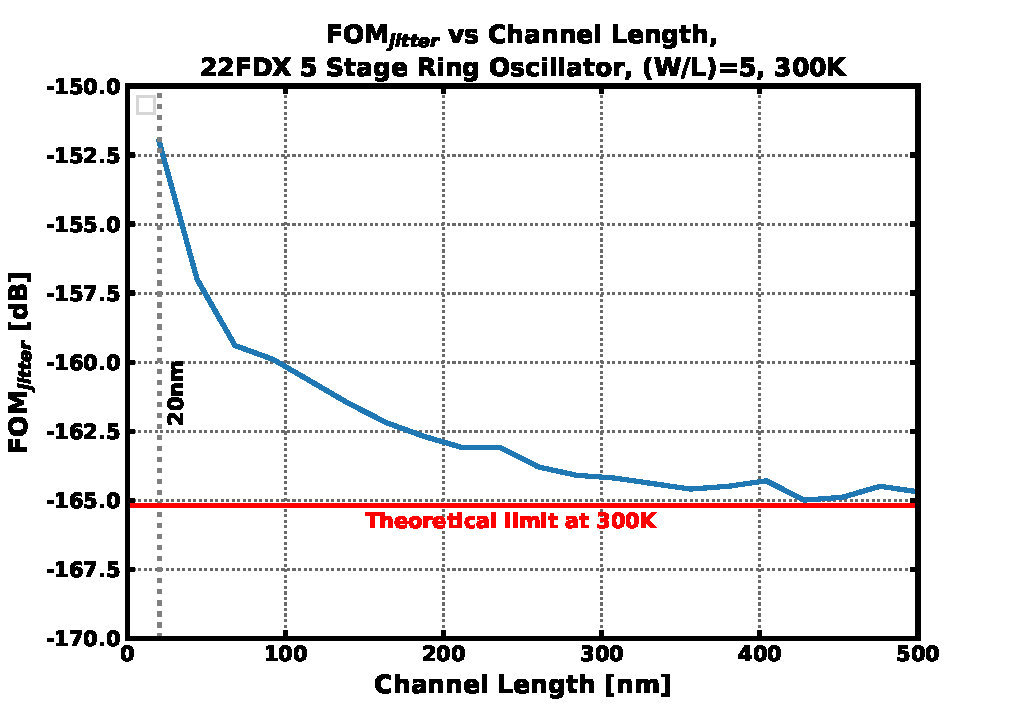
\includegraphics[width=1\textwidth, angle=0]{./figs/design/22fdx_rosc_fom}
		        \caption{ }
		        \label{fig:rosc_fom}
		    \end{subfigure}%
		    \begin{subfigure}{0.5\textwidth}
		        \centering
		        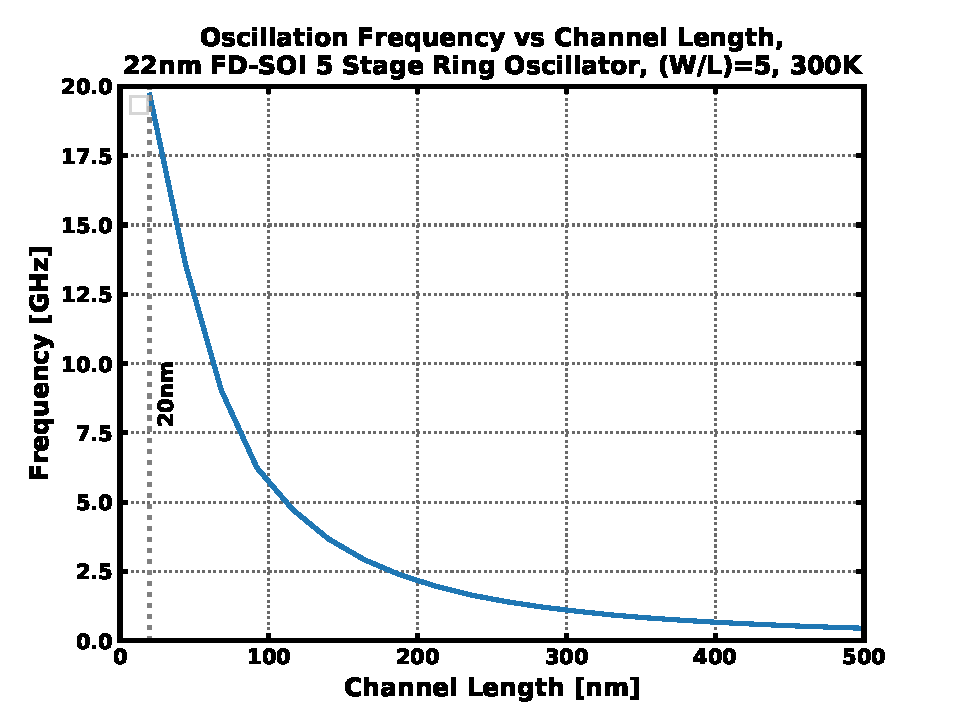
\includegraphics[width=1\textwidth, angle=0]{./figs/design/22fdx_rosc_freq}
		        \caption{ }
		        \label{fig:rosc_freq}
		    \end{subfigure}
		    % \caption{x.}
		    \label{fig:rosc_groupa}
		    \caption{22FDX ring oscillator channel length sweep versus \textbf{(a)} FOM, \textbf{(b)} Oscillation frequency.}
		\end{figure} 	

		\begin{figure}[htb!]
		    \centering
		    \begin{subfigure}{0.5\textwidth}
		        \centering
		        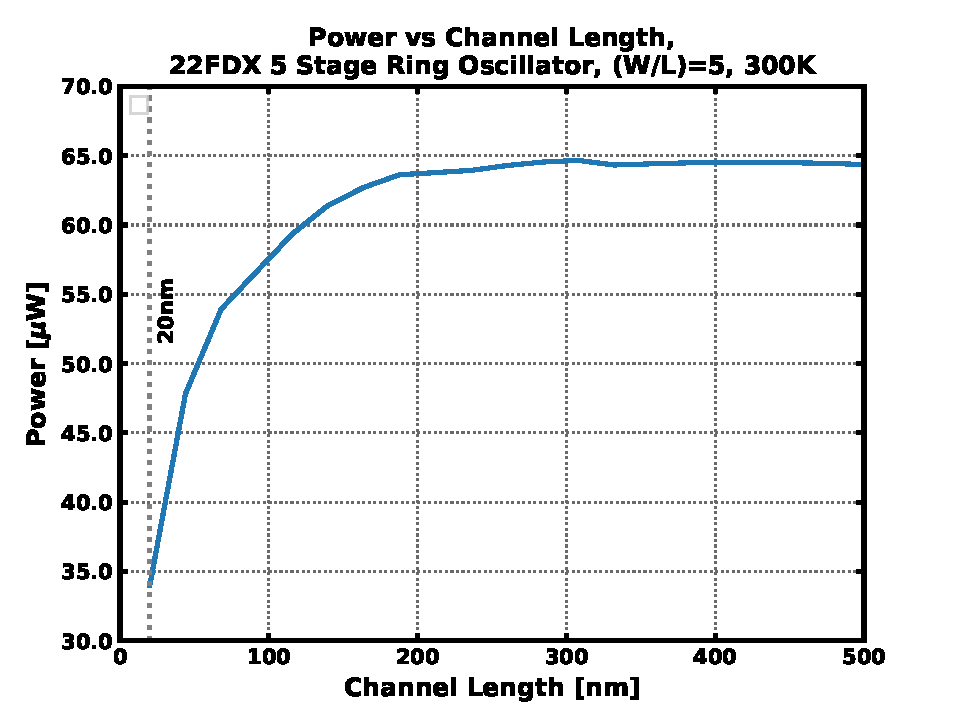
\includegraphics[width=1\textwidth, angle=0]{./figs/design/22fdx_rosc_power}
		        \caption{ }
		        \label{fig:rosc_power}
		    \end{subfigure}%
		    \begin{subfigure}{0.5\textwidth}
		        \centering
		        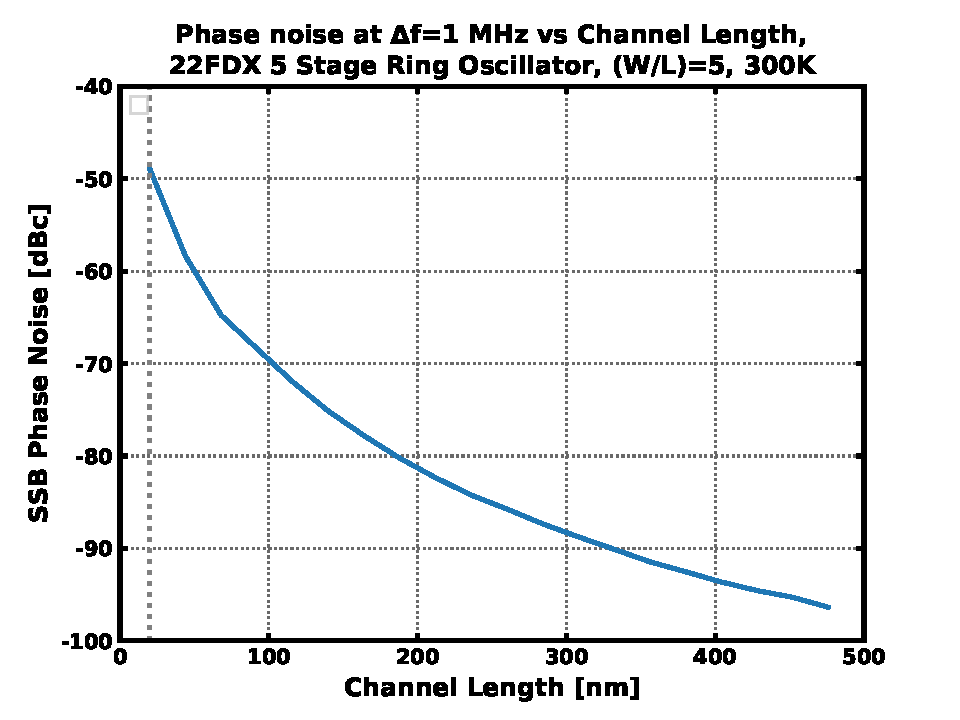
\includegraphics[width=1\textwidth, angle=0]{./figs/design/22fdx_rosc_pn_1mhz}
		        \caption{ }
		        \label{fig:rosc_groupb}
		    \end{subfigure}
		    % \caption{x.}
		    \label{fig:rosc_pn}
		    \caption{2FDX ring oscillator channel length sweep versus \textbf{(a)} Power, \textbf{(b)} Phase noise at 1 MHz carrier offset (SSB).}
		\end{figure} 



			\FloatBarrier
	\subsubsection{22FDX considerations}
		Idea: use backgates of FDSOI to tune frequency..
		Vth is approximately linear with applied backgate bias, use approximate model $vth = vth0 + \gamma V_{BS}$
		Derive that gmbs = $\gamma$ gm with this assumption. Gmbs and gm are easily found with SPICE simulator, which results in the extracted data below. 

		Although the BSIM-IMG FD-SOI threshold voltage model is not perfectly linear, it is observed that the body-bias threshold is approximately linear, especially under semi-local conditions. Thus, for simplified analysis, a new model for body-effect coupled threshold voltage is introduced here. Body bias is here defined as the potential $V_{BS}$ applied between the backgate contact and the source contact. 
		\begin{equation}
		V_{th} = V_{th0} - \gamma V_{BS}
		\end{equation}

		Might be challenging to achieve proper frequency and sufficient FOM, unfortunately....

		\begin{figure}[htb!]
		    \centering
		    \begin{subfigure}{0.5\textwidth}
		        \centering
		        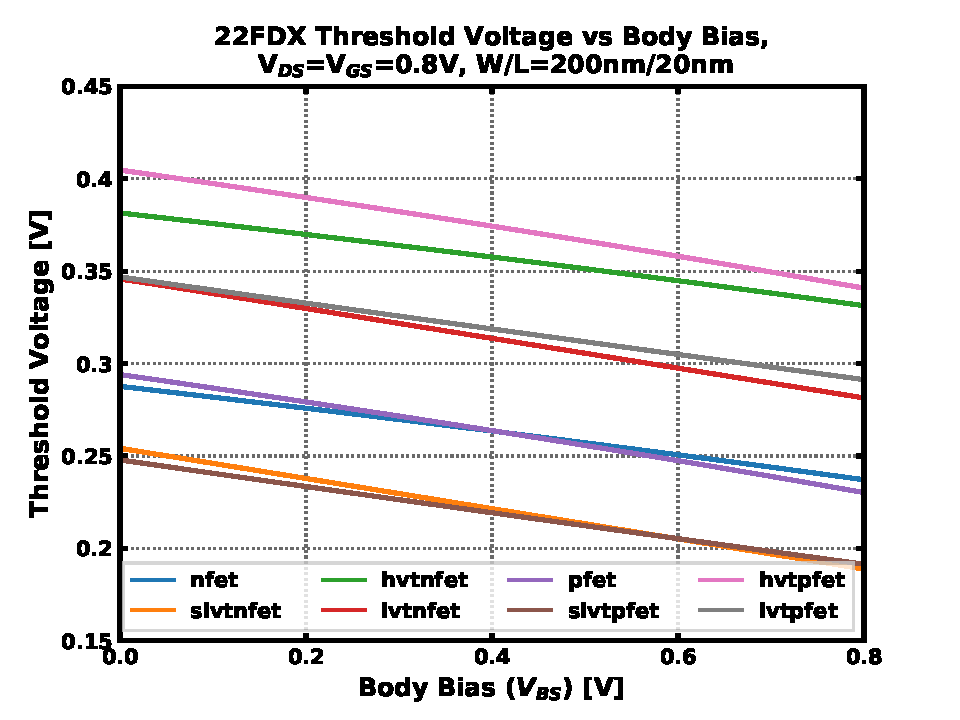
\includegraphics[width=1\textwidth, angle=0]{./figs/design/vth_vbs}
		        \caption{ }
		        \label{fig:vth_vs_vbs}
		    \end{subfigure}%
		    \begin{subfigure}{0.5\textwidth}
		        \centering
		        \includegraphics[width=1\textwidth, angle=0]{./figs/design/vth_slope_vbs}
		        \caption{ }
		        \label{fig:vth_slope_vs_vbs}
		    \end{subfigure}
		    % \caption{x.}
		    \label{fig:vth_groupa}
		    \caption{\textbf{(a)} 22 FDX threshold voltage versus body bias, \textbf{(b)} Rate of change of threshold voltage versus body bias.}
		\end{figure} 


		\begin{figure}[htb!]
		    \centering
		    \begin{subfigure}{0.5\textwidth}
		        \centering
		        \includegraphics[width=1\textwidth, angle=0]{./figs/design/vth}
		        \caption{ }
		        \label{fig:vth_vs_len}
		    \end{subfigure}%
		    \begin{subfigure}{0.5\textwidth}
		        \centering
		        \includegraphics[width=1\textwidth, angle=0]{./figs/design/gamma}
		        \caption{ }
		        \label{fig:gamma_vs_len}
		    \end{subfigure}
		    % \caption{x.}
		    \label{fig:vth_groupb}
		    \caption{\textbf{(a)} 22 FDX Extracted threshold voltage versus channel length, \textbf{(b)} Extracted body effect coefficient.}
		\end{figure} 


		Extracted vth and body effect coefficient ($\gamma$). Assuming gmbs = gamma*gm. Extracted for $V_{DD}=V_{GS}=0.4$. 

			\begin{table}[htb!]
				\centering
				\def\arraystretch{1.5}		
				\setlength\arrayrulewidth{1pt}
				\setlength{\tabcolsep}{1em} % for the horizontal padding
				\fontfamily{\sfdefault}\selectfont 
				\begin{tabular}{|l|l|l|l|l|}	
					\hline 
					\rule[-1ex]{0pt}{2.5ex} \cellcolor{gray!40}\textbf{Device} & \cellcolor{gray!40}\textbf{L [nm]} & \cellcolor{gray!40}\textbf{W [nm]} & \cellcolor{gray!40}\textbf{$V_{th}$ [mV]} & \cellcolor{gray!40}\textbf{$\gamma$ [mV/V]}\\ 
					\hline 
					\rule[-1ex]{0pt}{2.5ex} \textbf{nfet} & 20 & 100 & 306.3 & 59.14 \\ 
					\hline 
					\rule[-1ex]{0pt}{2.5ex} \textbf{nfet} & 100 & 500 & 376.4 & 65.4 \\ 
					\hline 
					\rule[-1ex]{0pt}{2.5ex} \textbf{slvtnfet} & 20n & 100 & 270.3 & 81.38 \\ 
					\hline 
					\rule[-1ex]{0pt}{2.5ex} \textbf{slvtnfet} & 100 & 500 & 326.7 & 83.23 \\ 
					\hline 
					\rule[-1ex]{0pt}{2.5ex} \textbf{hvtnfet} & 20n & 100 & 402.4 & 58.85 \\ 
					\hline 
					\rule[-1ex]{0pt}{2.5ex} \textbf{hvtnfet} & 100 & 500 & 513.5 & 61.96 \\ 
					\hline 
					\rule[-1ex]{0pt}{2.5ex} \textbf{lvtnfet} & 20 & 100 & 364.9 & 77.72 \\ 
					\hline 
					\rule[-1ex]{0pt}{2.5ex} \textbf{lvtnfet} & 100 & 500 & 466.3 & 74.85 \\ 
					\hline 
				\end{tabular} 
				\caption{22FDX core NFET threshold voltage and body effect coefficient extraction.}
				\label{nfet_vth_gamma}
			\end{table} 

			\begin{table}[htb!]
				\centering
				\def\arraystretch{1.5}		
				\setlength\arrayrulewidth{1pt}
				\setlength{\tabcolsep}{1em} % for the horizontal padding
				\fontfamily{\sfdefault}\selectfont 
				\begin{tabular}{|l|l|l|l|l|}	
					\hline 
					\rule[-1ex]{0pt}{2.5ex} \cellcolor{gray!40}\textbf{Device} & \cellcolor{gray!40}\textbf{L [nm]} & \cellcolor{gray!40}\textbf{W [nm]} & \cellcolor{gray!40}\textbf{$V_{th}$ [mV]} & \cellcolor{gray!40}\textbf{$\gamma$ [mV/V]}\\ 
					\hline 
					\rule[-1ex]{0pt}{2.5ex} \textbf{pfet} & 20 & 100 & 317.7 & 71.51 \\ 
					\hline 
					\rule[-1ex]{0pt}{2.5ex} \textbf{pfet} & 100 & 500 & 366.8 & 74.32 \\ 
					\hline 
					\rule[-1ex]{0pt}{2.5ex} \textbf{slvtpfet} & 20n & 100 & 272.6 & 71.09 \\ 
					\hline 
					\rule[-1ex]{0pt}{2.5ex} \textbf{slvtpfet} & 100 & 500 & 294.4 & 70.79 \\ 
					\hline 
					\rule[-1ex]{0pt}{2.5ex} \textbf{hvtpfet} & 20n & 100 & 430.7 & 71.28 \\ 
					\hline 
					\rule[-1ex]{0pt}{2.5ex} \textbf{hvtpfet} & 100 & 500 & 488.4 & 74.23 \\ 
					\hline 
					\rule[-1ex]{0pt}{2.5ex} \textbf{lvtpfet} & 20 & 100 & 374.2 & 69.93 \\ 
					\hline 
					\rule[-1ex]{0pt}{2.5ex} \textbf{lvtpfet} & 100 & 500 & 422.8 & 66.43 \\ 
					\hline 
				\end{tabular} 
				\caption{22FDX core PFET threshold voltage and body effect coefficient extraction.}
				\label{pfet_vth_gamma}
			\end{table} 	
\FloatBarrier



	\subsubsection{Ring oscillator frequency derivation}
		To analyze the oscillation frequency of a CMOS ring oscillator, an approximate model for a CMOS inverter will first be considered. A common model for delay in digital circuits [elmore delay model] is an RC circuit, where the MOSFET channels are approximated with an average conductance value $\langle g_{ch} \rangle$, and the output node is approximated to have a capacitance of C. With such a model, a ring oscillator would be assumed to have waveforms as decaying exponential, with time constant $\tau = \langle g_{ch} \rangle^{-1}C$, such as in Figure \ref{fig:rosc_rc}.
		\begin{figure}[htb!]
			\center\includegraphics[width=0.8\linewidth, angle=0]{figs/theory/osc_waves}
			\caption{Model for ring oscillator.}
			\label{fig:rosc_rc}
		\end{figure}

		\begin{figure}[htb!]
	        \centering
	        \begin{subfigure}{.5\textwidth}
	            \centering
	            \includegraphics[width=\linewidth]{figs/theory/inv_rc_model}
	            \caption{Inverter approximate model.}
	            \label{fig:rosc_3stg_cir}
	        \end{subfigure}%
	        \begin{subfigure}{.5\textwidth}
	            \centering
	            \includegraphics[width=0.8\linewidth]{figs/theory/inv_waves}
	            \caption{Inverter waveforms in ring oscillator.}
	            \label{fig:rosc_3stg_wave}
	        \end{subfigure}
	        \caption{Approximate model for ring oscillator inverter delay cell.}
	        \label{fig:rosc_3stg}
	    \end{figure}

		To calculate oscillation frequency ring oscillator from the RC model, several inferences are made:
		\begin{itemize}
			\item The switching point $V_M$ of the inverters is $V_{DD}/2$, based on the assumption that the NMOS and PMOS are of equal strength.
			\item The output of an inverter will have a decaying exponential which starts coincident with the passing of $V_M$ at the input.
			\item The propagation delay $t_{pd}$ for an inverter will be the time differential between the $V_M$ crossing points on the input and output.
			\item The oscillator frequency will be $f_{osc}$ = $1/2Nt_{pd}$, where N is the number of stages (i.e. defined by 2N propagation delays).
		\end{itemize}
			Following the definition of $V_M$, it is trivial to find that $t_{pd}$ = $\tau\ln2$. It is therefore known that:
		\begin{equation}
			f_{osc}^{-1} = 2Nt_{pd} = \frac{2\ln(2)NC}{\langle g_{ch}\rangle}
		\end{equation}

		\subsubsection{Finding $\langle g_{ch}\rangle$ and C}
			The node capacitance C is trivial to find based on the inverter gate capacitance and a lumped load capacitance term $C_L$:
			\begin{equation}
				C = C_{ox}\left ( W_N L_N + W_P L_N \right) + C_L
			\end{equation}
			The average channel conductance $\langle g_{ch} \rangle$ is more involved to find. To do so, several assumptions are made:
			\begin{itemize}
				\item L $>>$ L$_{min}$, so no velocity saturation, and therefore square law is applicable.
				\item NMOS and PMOS have equal $V_t$ and transconducance.
				\item Output transition occur with the active FET in saturation during $t_{pd}$. This requires:
				\begin{itemize}
					\item $V_{DD}/4 < V_{t} < V_{DD}/2$
				\end{itemize}
			\end{itemize}
			Following those assumptions, $\langle g_{ch} \rangle$ can be computed via integral within the period $t_{pd}$:
			\begin{equation}
				\langle g_{ch} \rangle = \frac{1}{t_{pd}} \int_0^{t_{pd}}\frac{I_{out}(t)}{V_{out}(t)}dt
			\end{equation}
			$I_{out}$ is computed using the saturated MOSFET square law model an exponential waveforms assumptions. An $I_{short}$ term is included to account for output current reduction from short-circuit conduction.
			\begin{equation}
				I_{out}(t) = \frac{k_n}{2}\left(\frac{W}{L}\right)_n\left[\left(V_{in}(t) - V_t\right)^2 \right]  - I_{short} = \frac{k_n}{2}\left(\frac{W}{L}\right)_n\left[\left(V_{DD}\left(1-e^{-t/\tau}\right) - V_t\right)^2 - \left(\frac{V_{DD}}{2} -V_t\right)^2\right]
			\end{equation}
			$k_n = \mu_nC_{ox}$, with the equal PMOS/NMOS assumption, $k_n\left(\frac{W}{L}\right)_n=k_p\left(\frac{W}{L}\right)_p$. $V_{out}$ is simply a decaying exponential with a delay $t_pd$ versus the input:
			\begin{equation}
				V_{out} = V_{DD}e^{-(t-t_{pd})/\tau}
			\end{equation}
			Now, computing the integral for $\langle g_{ch} \rangle$ yields:
			\begin{equation}
				\langle g_{ch} \rangle = \frac{1}{2}\mu_nC_{ox}\left(\frac{W}{L}\right)_n\left[V_{DD}\left(\frac{7}{8\ln2}-1\right)-V_t\left(\frac{1}{\ln2}-1\right) \right]
			\end{equation}
			As a simplification, $\alpha$ is defined as:
			\begin{equation}
				\alpha = \left[V_{DD}\left(\frac{7}{8\ln2}-1\right)-V_t\left(\frac{1}{\ln2}-1\right) \right]
			\end{equation}	
		
		\subsubsection{Handling unequal NMOS/PMOS}
			In the case of different threshold voltages for NMOS and PMOS:
			\begin{equation}
				f_{osc}^{-1} = N(t_{pdn} + t_{pdp}) = \ln(2)NC\left(\frac{1}{\langle g_{ch}\rangle_n} + \frac{1}{\langle g_{ch}\rangle_p}\right) = \frac{2\ln(2)NC}{\langle g_{ch}\rangle'}
			\end{equation}	
			A modified $\langle g_{ch}\rangle'$ is defined:
			\begin{align}
				\langle g_{ch}\rangle' = 2\left(\frac{1}{\langle g_{ch}\rangle_n} + \frac{1}{\langle g_{ch}\rangle_p}\right)^{-1} = 2\frac{\langle g_{ch}\rangle_n \langle g_{ch}\rangle_p}{\langle g_{ch}\rangle_n + \langle g_{ch}\rangle_p}
				= 2\frac{\frac{1}{2}\mu_nC_{ox}\left(\frac{W}{L}\right)_n \alpha_n\frac{1}{2}\mu_pC_{ox}\left(\frac{W}{L}\right)_p \alpha_p}{\frac{1}{2}\mu_nC_{ox}\left(\frac{W}{L}\right)_n\alpha_n + \frac{1}{2}\mu_pC_{ox}\left(\frac{W}{L}\right)_p\alpha_p}
			\end{align}	
			This is somewhat unmanagable, however enforcing $\mu_nC_{ox}\left(\frac{W}{L}\right)_n = \mu_pC_{ox}\left(\frac{W}{L}\right)_p$ for $V_M$ to equal $V_{DD}/2$ gives:
			\begin{align}
				\langle g_{ch}\rangle' = \frac{1}{2}\mu_nC_{ox}\left(\frac{W}{L}\right)_n\frac{2 \alpha_n\alpha_p}{\alpha_n + \alpha_p} = \frac{1}{2}\mu_nC_{ox}\left(\frac{W}{L}\right)_n \alpha'
			\end{align}	
			Thus $\alpha_n$ and $\alpha_p$ are found for the according threshold voltages and then $\langle g_{ch}\rangle$ can be found.
			\begin{equation}
				\alpha' =  \frac{2 \alpha_n\alpha_p}{\alpha_n + \alpha_p}
			\end{equation}

		\subsubsection{Solving for oscillator frequency and power}
			Solving for oscillator frequency:
			\begin{equation}
				f_{osc} = \frac{\mu_nC_{ox}}{4\ln2NC}\left(\frac{W}{L}\right)_n\left[V_{DD}\left(\frac{7}{8\ln2}-1\right)-V_t\left(\frac{1}{\ln2}-1\right) \right]
			\end{equation}
			If gate capacitance is the dominant load component, and PMOS/NMOS are equal sized such that $C=2WLC_{ox}$:
			\begin{equation}
				f_{osc} = \frac{\mu_n}{8\ln2N}\cdot\frac{1}{L^2}\left[V_{DD}\left(\frac{7}{8\ln2}-1\right)-V_t\left(\frac{1}{\ln2}-1\right) \right]
			\end{equation}
			Power can also be calculated, knowing in digital circuits $P = fC_{\Sigma}V_{DD}^2$, where $C_{\Sigma}$ is the total active capacitance. Thus:
			\begin{equation}
				P_{osc} = Nf_{osc}CV_{DD}^2 = \frac{\mu_nC_{ox}}{4\ln2}\left(\frac{W}{L}\right)_n\left[V_{DD}\left(\frac{7}{8\ln2}-1\right)-V_t\left(\frac{1}{\ln2}-1\right) \right]
			\end{equation}
			It should be noted that the power consumption is proportional to FET aspect ratio (W/L).

	\subsubsection{Ring oscillator backgate tuning derivation}
		Using the basic expressions for ring oscillator frequency, the operature under backgate biasing can be found. In UTBB-FDSOI processes, the threshold voltage of a FET varies with linear dependence on the applied back gate bias $V_{BG}$ (relative to source). Given the body effect coefficient of a process, $\gamma$, $V_t$ is:
		\begin{equation}
			V_t = V_{t0} - \gamma V_{BG}
		\end{equation}
		Using this in the ring oscillator frequency equation:
		\begin{equation}
			f_{osc} = \frac{\mu_nC_{ox}}{4\ln2NC}\left(\frac{W}{L}\right)_n\left[V_{DD}\left(\frac{7}{8\ln2}-1\right)-V_{t0}\left(\frac{1}{\ln2}-1\right) + \gamma V_{BG}\left(\frac{1}{\ln2}-1\right) \right]
		\end{equation}
		Equivalently, $f_{osc} = f_{0,osc} + \Delta f_{osc}(V_{BG})$, where:
		\begin{equation}
			\Delta f_{osc}(V_{BG}) = \gamma V_{BG}\frac{\mu_nC_{ox}}{4\ln2NC}\left(\frac{W}{L}\right)_n\left[\frac{1}{\ln2}-1\right]
		\end{equation}	
		And $f_{0,osc}$ is the frequency with no backgate bias. If the backgate is swept from 0 to $V_{DD}$, and the node capacitance is increasingly varied (C0 to C3), Figure \ref{fig:rosc_tuning} is observed. Note that the change in frequency is linear with to backgate bias.
		\FloatBarrier
		\begin{figure}[htb!]
			\center\includegraphics[width=0.3\linewidth, angle=0]{figs/backgate_rosc_tuning2.pdf}
			\caption{Backgate-tuned ring oscillator with coarse tuning capacitor bank.}
			\label{fig:rosc_tuning}
		\end{figure}
		If the backgate voltage is constrained in the range [0, $V_{DD}$], the center frequency $f_c$ in the tuning range of the oscillator is then:
		\begin{equation}
			f_{c} = \frac{\mu_nC_{ox}}{4\ln2NC}\left(\frac{W}{L}\right)_n\left[V_{DD}\left(\frac{7}{8\ln2}-1+\frac{\gamma}{2\ln2}-\frac{\gamma}{2}\right)-V_{t0}\left(\frac{1}{\ln2}-1\right)\right]
		\end{equation}
		The tuning range is also therefore:
		\begin{equation}
			\Delta f = \gamma V_{DD}\frac{\mu_nC_{ox}}{4\ln2NC}\left(\frac{W}{L}\right)_n\left[\frac{1}{\ln2}-1\right]
		\end{equation}
		The fractional tuning range of the oscillator is:
		\begin{equation}
			\frac{\Delta f}{f_c} = \frac{\gamma V_{DD}\left( 1-\ln2 \right)}{V_{DD}\left(\frac{7}{8}-\ln2+\frac{\gamma}{2}-\frac{\gamma}{2}\ln2\right)-V_{t0}\left(1-\ln2\right)}
		\end{equation}	
		If a N-bit DAC is used to control the oscillator, the resulting DCO gain is therefore:
		\begin{equation}
			K_{DCO} = \frac{\Delta f}{2^{N_{DAC}}} = \frac{f_c}{2^{N_{DAC}}}\cdot\frac{\gamma V_{DD}\left( 1-\ln2 \right)}{V_{DD}\left(\frac{7}{8}-\ln2+\frac{\gamma}{2}-\frac{\gamma}{2}\ln2\right)-V_{t0}\left(1-\ln2\right)}
		\end{equation}	
	\subsubsection{DCO Gain Uncertainty}
		The DCO gain $K_{DCO}$ is used in setting the loop filter coefficients, so the uncertainty of the DCO gain is of interest to allow for statistical analysis of the PLL across process variation. The uncertainty of $K_{DCO}$ (normalized with nominal $K_{DCO}$ value) as a function of $V_{DD}$, $V_{t0}$ and $\gamma$ is:
		\begin{equation}
			\sigma_{KDCO} = \sqrt{\left(\frac{\partial K_{DCO}}{\partial V_{DD}}\cdot\frac{\sigma_{VDD}}{K_{DCO}} \right)^2 + \left(\frac{\partial K_{DCO}}{\partial V_{t0}}\cdot\frac{\sigma_{Vt0}}{K_{DCO}} \right)^2 + \left(\frac{\partial K_{DCO}}{\partial \gamma}\cdot\frac{\sigma_\gamma}{K_{DCO}} \right)^2}
		\end{equation}

		\begin{align}
			\frac{\partial K_{DCO}}{\partial V_{DD}} &= \frac{f_c}{2^{N_{DAC}+1}}\cdot\frac{-\gamma V_{t0}(1-\ln2)^2}{\left[ V_{DD}\left(\frac{7}{8}-\ln2+\frac{\gamma}{2}-\frac{\gamma}{2}\ln2\right)-V_{t0}\left(1-\ln2\right) \right]^2}\\
			\frac{\partial K_{DCO}}{\partial V_{t0}} &= \frac{f_c}{2^{N_{DAC}+1}}\cdot\frac{\gamma V_{DD}(1-\ln2)^2}{\left[ V_{DD}\left(\frac{7}{8}-\ln2+\frac{\gamma}{2}-\frac{\gamma}{2}\ln2\right)-V_{t0}\left(1-\ln2\right) \right]^2}\\
			\frac{\partial K_{DCO}}{\partial \gamma} &= \frac{f_c}{2^{N_{DAC}+1}}\cdot\frac{V_{DD}\cdot(1-\ln2) \left[ V_{DD}\left(\frac{7}{8}-\ln2\right)-V_{t0}\left(1-\ln2\right) \right]}{\left[ V_{DD}\left(\frac{7}{8}-\ln2+\frac{\gamma}{2}-\frac{\gamma}{2}\ln2\right)-V_{t0}\left(1-\ln2\right) \right]^2}
		\end{align}
		Simplified:
		\begin{multline}
			\sigma_{KDCO} = \frac{1}{\gamma V_{DD} \left[ V_{DD}\left(\frac{7}{8}-\ln2+\frac{\gamma}{2}-\frac{\gamma}{2}\ln2\right)-V_{t0}\left(1-\ln2\right) \right]}\cdot\\ \sqrt{\left(\gamma V_{t0} (1-\ln2)\sigma_{VDD} \right)^2 + \left(\gamma V_{DD} (1-\ln2)\sigma_{Vt0} \right)^2 + \left( V_{DD}\left[ V_{DD}\left(\frac{7}{8}-\ln2\right)-V_{t0}\left(1-\ln2\right) \right]\sigma_{\gamma} \right)^2 }
		\end{multline}		
		\hl{Motivate selection of fine backgate tuning and supply coarse tuning (as future extension?). I.e. what is df/dVdd vs df/dVbg?}
		\hl{\textbf{TODO} - extract $\gamma$, $V_{t0}$ variance for FETs in process kit, place in results?}
		\subsubsection{DCO Sensitivity}
		The frequency tuning sensitivity of the ring oscillator for supply and backgate voltages will be compared. First the following is defined, following that the derived equations for oscillator frequency are linear.
		\begin{equation}
			f_{osc}(V_{DD}+\Delta V_{DD}) = f_{osc}(V_{DD}) + f_{osc}(\Delta V_{DD})
		\end{equation}
		\begin{equation}
			f_{osc}(V_{DD}) = f_0
		\end{equation}
		\begin{equation}
			f_{osc}(\Delta V_{DD}) = \Delta f
		\end{equation}

		In the case of supply voltage tuning, the change (proportion) of frequency per voltage of applied extra bias is (evaluated at zero back-gate bias):
		\begin{equation}
			S^{f_{osc}}_{V_{DD}} = \frac{\Delta f}{f_0}\cdot\frac{1}{\Delta V_{DD}}  = \frac{\left(\frac{7}{8\ln2}-1\right)}{V_{DD}\left(\frac{7}{8\ln2}-1\right)-V_{t0}\left(\frac{1}{\ln2}-1\right)}
		\end{equation}
		With $V_{DD}$=0.8, $V_{t0}$=0.3, it is expected 340\% change in frequency will result per extra volt of applied bias (of course, this is linearized, one does not expect to apply an extra 1V). Realistically, the supply can be tuned $\pm$ 10\%, which corresponds to a $\pm$27.2\% tuning range of the oscillator. This is perhaps a good coarse tuning mechanism, but does not provide much for fine tuning. \hl{make note of supply noise sensitivity!}

		\par In the case of backgate tuning, the change (proportion) of frequency per volt of applied backgate bias is:
		\begin{equation}
			S^{f_{osc}}_{V_{BG}} = \frac{\Delta f}{f_0}\cdot\frac{1}{\Delta V_{BG}}  = \frac{\gamma \left(\frac{1}{\ln2}-1\right)}{V_{DD}\left(\frac{7}{8\ln2}-1\right)-V_{t0}\left(\frac{1}{\ln2}-1\right)}
		\end{equation}

		With $\gamma$=0.07, $V_{DD}$=0.8, $V_{t0}$=0.3, it is expected a 40\% change in frequency will result per volt applied of backgate bias. This is much finer than achieved with supply voltage tuning. The ratio of frequency sensitivity to supply and backgate voltage tuning is:

		\begin{equation}
			\frac{S^{f_{osc}}_{V_{DD}}}{S^{f_{osc}}_{V_{BG}}} =  \frac{\frac{7}{8\ln2}-1}{\gamma \left(\frac{1}{\ln2}-1\right)}
		\end{equation}
		Under the aforementioned biasing conditions, it is expected that 8.4x finer control can be achieved with backgate tuning. The wide backgate voltage ranges allowed for with FDSOI technology permit for design of a voltage-DAC based controll scheme which will achieve far smaller frequency resolution than with supply voltage tuning. 

		\subsubsection{temp}
			\begin{itemize}[itemsep=4pt,label=\protect---]
				\item Simulated 5 stage ring oscillator.
				\item RVT devices, W/L = 5.
				\item Ran pss/pnoise.
				\item Computed FOM vs channel length (lower is better):
			\end{itemize}
				\begin{equation}
					\textnormal{FOM} = 10\log_{10}\left( \left( \frac{\Delta f}{f_0} \right)^2 \cdot\frac{\textnormal{P}_{total}}{\textnormal{1 mW}} \right)\hspace{1em} \textnormal{[dB]}
				\end{equation}
			\begin{itemize}[itemsep=4pt,label=\protect---]
				\item It is seen that FOM improves asymptotically to $\sim$ -165 with longer L.
				\item FOM < -160 dB $\rightarrow$ L $\geq$ 100 nm.
				\item L should be set as long as possible, while mantaining appropriate speed.
				\begin{itemize}[itemsep=4pt,label=$\bullet$]
					\item This is actually recommended in Razavi's new book \cite{Razavi2020}.
				\end{itemize}
			\end{itemize}



		\subsubsection{Delay cell}

			\begin{itemize}[itemsep=4pt,label=\protect---]
				\item Utilize pseudo-differential inverter stage [3], in parallel with back gate tuned inverter.
				\begin{itemize}[itemsep=4pt,label=$\bullet$]
					\item Pseudo-differential stage couples oscillators, forcing crossing voltage $V_{DD}/2$.
					\item Back gate tuned oscillator used to adjust frequency.
				\end{itemize}			
				\item Ratioing the sizes two types of inverters can be used to adjust the VCO gain. A ratio of 1:1 should reduce the $K_{VCO}$ in half from what is expected from theory, a ratio of 3:1 (with pseudo-diff inverters being larger) will reduce $K_{VCO}$ by 4. 
				\item \textbf{Requires complementary control of backgate voltage for tuning.}
				\item \textbf{\color{red}Allows for 0-$V_{DD}$ control range.	}
			\end{itemize}

			\begin{figure}[htb!]
			        \centering
			        \includegraphics[width=0.8\textwidth, angle=0]{./figs/parallel_delay_cell}
			    % \caption{Approximate model for ring oscillator inverter delay cell.}
			\end{figure}


			\begin{itemize}[itemsep=4pt,label=\protect---]
				\item Must use devices in N well (PFET, HVTPFET, SLVTNFET, LVTNFET) to not forward bias substrate diode.
				\item To achieve $V_{m}$ =  $V_{DD}/2$, PFET + LVTNFET give most reasonable W$_P$/W$_N$, ca 1.2-1.4.
				\begin{itemize}[itemsep=4pt,label=$\bullet$]
					\item SLVTNFET + PFET needs W$_P$/W$_N$ $\approx$ 8.
				\end{itemize}
			\end{itemize}


			\begin{figure}[htb!]
			    \centering
			    \begin{subfigure}{0.5\textwidth}
			        \centering
			        \includegraphics[width=1\textwidth, angle=0]{./figs/design/ratio_lvtnfet_pfet}
			        \caption{ }
			        \label{fig:ratio_lvtn_p}
			    \end{subfigure}%
			    \begin{subfigure}{0.5\textwidth}
			        \centering
			        \includegraphics[width=1\textwidth, angle=0]{./figs/design/ratio_slvtnfet_pfet}
			        \caption{ }
			        \label{fig:ratio_slvtn_p}
			    \end{subfigure}
			    % \caption{x.}
			    \label{fig:opt_ratio}
			    \caption{\textbf{(a)} Optimal width PFET/LVTNFET, \textbf{(b)} Optimal width PFET/SLVTNFET.}
			\end{figure} 


			\begin{itemize}[itemsep=4pt,label=\protect---]
				\item Good symmetry of rise time observed, with $V_{cm}$ close to $V_{DD}/2$ over the full oscillation cycle.
				\item \textbf{Observed 10.3\% fractional frequency tuning with L=150nm, FOM=-161 dB, 1:1 ratio of inverters.}
				\item I require $<$ 1\% fractional tuning range to achieve my $K_{DCO}$ with a 10b DAC, this will not work. The (W/L) becomes large to achieve a high inverter ratio, thus increases power too much.
			\end{itemize}

			\hspace{1em}\textbf{Single ended outputs:}
			\vspace{-1em}
			\begin{figure}[htb!]
			        \centering
			        \includegraphics[width=0.7\textwidth, angle=0]{./figs/parallel_osc_wfm}
			    % \caption{Approximate model for ring oscillator inverter delay cell.}
			\end{figure}
			\vspace{-1em}
			\hspace{1em}\textbf{Common mode voltage:}
			\vspace{-1em}
			\begin{figure}[htb!]
			        \centering
			        \includegraphics[width=0.7\textwidth, angle=0]{./figs/parallel_cmv}
			    % \caption{Approximate model for ring oscillator inverter delay cell.}
			\end{figure}


			\begin{itemize}[itemsep=4pt,label=\protect---]
				\item Modify the pseudo-differential cell to have header/footer transistors with back gate control.
				\begin{itemize}[itemsep=4pt,label=$\bullet$]
					\item Cross-coupled devices force differential operation
					\item Header/footer devices used to adjust frequency.
				\end{itemize}				
				\item Ratioing the size of the header/footer devices to the size of the cross-coupling devices tunes $K_{VCO}$
				\item \textbf{Requires complementary control of backgate voltage for tuning.}
			\end{itemize}

			\begin{figure}[htb!]
			        \centering
			        \includegraphics[width=0.58\textwidth, angle=0]{./figs/tele_delay_cell}
			    % \caption{Approximate model for ring oscillator inverter delay cell.}
			\end{figure}


			\begin{itemize}[itemsep=4pt,label=\protect---]
				\item Good symmetry of rise time observed, with $V_{cm}$ close to $V_{DD}/2$ over the full oscillation cycle.
				\item $W_p$/$W_n$ = 1.25. Nominal (W/N)$_n$ = 400n/150n
				\item \textbf{1:1 ratioing: Observed 10.0\% fractional frequency tuning with L=150nm, {\color{red}FOM=-162.6 dB.}}
				\item \textbf{1:2 ratioing (header/footer larger): Observed 4.8\% fractional frequency tuning with L=150nm.}
				\item Still hard to get required $<$ 1\% fractional frequency tuning.
			\end{itemize}

			% \begin{figure}[htb!]
			%         \centering
			%         \includegraphics[width=0.8\textwidth, angle=0]{./figs/telescopic_wfm}
			%     % \caption{Approximate model for ring oscillator inverter delay cell.}
			% \end{figure}



			\begin{itemize}[itemsep=4pt,label=\protect---]
				\item Not as linear as I had hoped, $K_{VCO}$ decreases by -33\% when $V_{DD}$ is swept [0, 0.8] V.
				\item I have observed a decease in $\gamma$ at higher back gate biases, this and mobility degredation(??) might explain this trend.
			\end{itemize}

			\begin{figure}[htb!]
			        \centering
			        \includegraphics[width=0.8\textwidth, angle=0]{./figs/telescopic_kcvo_vbg}
			    % \caption{Approximate model for ring oscillator inverter delay cell.}
			\end{figure}


			% \vspace{100em}
			\begin{itemize}[itemsep=4pt,label=\protect---]
				\item PVT (coarse), medium and fine tuning all need to coexist (overlap in frequency).
				\item PVT tuning achieved with bank of differentially connected capacitors
				\item Fine/medium tuning achieved with parallel combination of header/footer transistors. The ratio of these devices affects the difference of the ranges.

			\end{itemize}


			\begin{figure}[htb!]
			        \centering
			        \includegraphics[width=0.65\textwidth, angle=0]{./figs/telescopic_pseudodiff_delay_cell_all_tune}
			    % \caption{Approximate model for ring oscillator inverter delay cell.}
			\end{figure}

			\begin{figure}[htb!]
			    \centering
			    \begin{subfigure}{0.5\textwidth}
			        \centering
			        \includegraphics[width=1\textwidth, angle=0]{./figs/results/osc_se_waves}
			        \caption{ }
			        \label{fig:osc_se_waves}
			    \end{subfigure}%
			    \begin{subfigure}{0.5\textwidth}
			        \centering
			        \includegraphics[width=1\textwidth, angle=0]{./figs/results/osc_cmv}
			        \caption{ }
			        \label{fig:osc_cmv}
			    \end{subfigure}
			    % \caption{x.}
			    \label{fig:osc_waves}
			    \caption{\textbf{(a)} Oscillator single-ended waveforms, \textbf{(b)} Oscillator common mode voltage waveform.}
			\end{figure} 


		\subsection{Full circuit}
		\subsubsection{Layout}
% ################################################################################################
% ################################################################################################
	\FloatBarrier
	\subsection{CDAC}
		\subsubsection{Circuit}
			\begin{figure}[htb!]
			        \centering
			        \includegraphics[width=\textwidth, angle=0]{./figs/cdac_10b}
			    % \caption{Approximate model for ring oscillator inverter delay cell.}
			\end{figure}
		\subsubsection{Layout}





% ################################################################################################
% ################################################################################################
	\FloatBarrier
	\subsection{Logic}





			\begin{itemize}[itemsep=4pt,label=\protect---]
			        \item Phase error zeroing reset implemented.
			        \item Reset asserted (synchronously) for single cycle 
					\begin{itemize}[itemsep=4pt,label=$\bullet$]
						\item DCO reset is at de-assertion of RST
						\item Logic is reset at clock edge at end of RST assertion
					\end{itemize}
					\item Allows for physical oscillator phase and digital phase error variable to be simulataneously set to zero.
					\begin{itemize}[itemsep=4pt,label=$\bullet$]
						\item Also BBPD doesn't work with BOTH phase/frequency error.
					\end{itemize}
					\item Should enable faster lock (only initial unknown is frequency).
					\item Really only possible with the ring oscillator (LC can't start instantly)
			\end{itemize}

			\textbf{\hspace{3em}Reset scheme}
			\begin{figure}[htb!]
			        \centering
			        \includegraphics[width=0.8\textwidth, angle=0]{./figs/pll_reset}
			    % \caption{Approximate model for ring oscillator inverter delay cell.}
			\end{figure}



			\begin{itemize}[itemsep=4pt,label=\protect---]
			        \item Controller consists of 5 state FSM
					\begin{enumerate}[itemsep=4pt,label=\arabic*]
						\item Calibration
						\item Run PLL, synchronous counter (timed start-up)
						\item \textbf{Run PLL, BBPD} 
						\item Sleep (triggered externally)
						\item PLL restore (when sleep de-asserted)
					\end{enumerate}
					\item Calibration also has FSM, which implements a frequency-error minimizing algorithm 
					\begin{itemize}[itemsep=4pt,label=$\bullet$]
						\item Starts at lowest capbank code, increments until argmin.
						\item Frequency error by integrating error out over a number of cycles
						\item Freq. resolution = $f_{ref}$/$N_{cycles}$
						\item $N_{cycles}$ = 4 yields 0.5\% fractional resolution (vs cap bank resolution of 1.2\%)
					\end{itemize}
			\end{itemize}

			\begin{figure}[htb!]
			        \centering
			        \includegraphics[width=0.9\textwidth, angle=0]{./figs/pll_asm}
			    % \caption{Approximate model for ring oscillator inverter delay cell.}
			\end{figure}


		\subsubsection{Circuit}
		\subsubsection{Layout}

			\begin{itemize}[itemsep=4pt,label=\protect---]
			        \item Total area for logic = 716$\mu m^2$.
			        \item Layout in 30 x 40 $\mu m$, ca. 50 \% density.
			        \item Power = 31.4 $\mu$W at 0.65V (82\% leakage).
			        \item Need to test at 0.5V, should be acceptable
			        \item Need to replace pins (when fully decided)
			\end{itemize}

			\begin{figure}[htb!]
			        \centering
			        \includegraphics[width=0.6\textwidth, angle=0]{./figs/pnr_digital}
			    % \caption{Approximate model for ring oscillator inverter delay cell.}
			\end{figure}










% ################################################################################################
% ################################################################################################
	\FloatBarrier
	\subsection{Output buffer}
		\subsubsection{Circuit}
		\subsubsection{Layout}


			\begin{itemize}[itemsep=4pt,label=\protect---]
				\item \textbf{Edge time out of ring oscillator is slow.} Slow edge time allows noise to couple to phase:
				% \begin{equation}
					% t_{10-90} = \frac{1.1}{\ln 2 N f_{ref}}
				% \end{equation}
				\begin{equation}
					\Delta \Phi = 2\pi f_{osc}\left(\frac{dV}{dT}\right)^{-1}\cdot\Delta V
				\end{equation}
				\item For good phase detector performance and to avoid effects of external loading, buffers are needed.
				\item Highest noise susceptibility when crossing $V_{CM}$.
				\item If $A_i$ is the inverter gain at $V_{CM}$, the pseudodifferential buffer stage here will provide the following CMRR:
				\begin{equation}
				CMRR = \left|\frac{1+\gamma A_i}{1-\gamma A_i}\right|
				\end{equation}
				\item Conveniently in 22FDX, $\gamma$ = 0.075 and $A_i \approx$ 14 with min. length PFET+LVTNFET at $V_{DD}=0.8$. \textbf{Thus CMRR = 26 dB.} This should help reject supply noise.
				\item Longer L yield essentially 0 dB CMRR. 

			\end{itemize}

			\begin{figure}[htb!]
			        \centering
			        \includegraphics[width=0.8\textwidth, angle=0]{./figs/pseudiff_buffer}
			    % \caption{Approximate model for ring oscillator inverter delay cell.}
			\end{figure}


% ################################################################################################
% ################################################################################################
	\FloatBarrier
	\subsection{Synchronous Counter}
		\begin{itemize}[itemsep=4pt,label=\protect---]
			\item Two choices for coarse linear phase detector, delay line TDC or synchronous counter.

				\item \textbf{Coarse delay line TDC}
				\begin{itemize}
					\item {\color{red}\textbf{(-)}} Complexity grows as $\mathcal{O}(n)$.
					\item {\color{red}\textbf{(-)}} Requires calibration of delay cells (possibly slow).
					\item {\color{red}\textbf{(-)}} Linearity issues, with poor calibration, gain accuracy is a problem.
					\item {\color{red}\textbf{(-)}} Needs divider.
				\end{itemize}

				\item \textbf{Synchronous counter}
				\begin{itemize}
					\item {\color{teal}\textbf{(+)}} Complexity grows as $\mathcal{O}(log(n))$.
					\item {\color{teal}\textbf{(+)}} No calibration, no linearity issues.
					\item {\color{teal}\textbf{(+)}} Divider not needed (reduces noise, power?).
					\item {\color{red}\textbf{(-)}} High power, must run as oscillator frequency.
					\item {\color{red}\textbf{(-)}} Resolution limited be to equal to divider modulus.
				\end{itemize}
			\item Counter approach has \textit{significant} advantages for PLL start up. Will switch of counter after initial lock to save power.
		\end{itemize} 	
		\subsubsection{Circuit}
			\begin{itemize}[itemsep=4pt,label=\protect---]
				\item Only tested ripple (asynchronous) counter last time. 
				\item Implement T flip-flop with XOR gate, AND carry logic. Logic implemented as NAND2 only, with all FETS 200nm/20nm. 
				\item Necessary to ensure that incorrect value isn't sampled, which is possible with asynchronous during ripple period. Penalty: 50 NAND2 gates, all FF's must be clocked every input cycle, i.e. more power than async.
			\end{itemize}
			% \vspace{-3em}
			\begin{figure}[htb!]
			        \centering
			        \includegraphics[width=1\textwidth, angle=0]{./figs/sync_counter.pdf}
			    % \caption{Approximate model for ring oscillator inverter delay cell.}
			\end{figure}


			\textbf{Count to phase error decoder}
			\begin{figure}[htb!]
			        \centering
			        \includegraphics[width=0.8\textwidth, angle=0]{./figs/sc_decoder}
			    % \caption{Approximate model for ring oscillator inverter delay cell.}
			\end{figure}

		\subsubsection{Layout}


% ################################################################################################
% ################################################################################################
\FloatBarrier
